\documentclass[a4paper,11pt,twoside]{report}
\usepackage[a4paper,left=2cm,right=2cm,top=3cm,bottom=3cm,bindingoffset=5mm]{geometry}
\setlength{\headheight}{13.6pt}
\usepackage[ngerman]{babel}
\usepackage[utf8]{inputenc}
\usepackage{graphicx}
\usepackage{caption}
\usepackage{subcaption}
\usepackage{fixltx2e}
\usepackage{lastpage}
\usepackage{epstopdf}
\graphicspath{outdir=/u/mhemmer/Documents/Theses/BachelorArbeit/}
\usepackage{fancyhdr}
\usepackage{amsmath}
\usepackage{amsthm}
\usepackage{amsbsy}
\usepackage{amssymb}
\usepackage{hyperref}
\usepackage{multirow}
\usepackage[toc,page]{appendix}

\usepackage{mathtools}
\DeclarePairedDelimiter\bra{\langle}{\rvert}
\DeclarePairedDelimiter\ket{\lvert}{\rangle}
\DeclarePairedDelimiterX\braket[2]{\langle}{\rangle}{#1 \delimsize\vert #2}
\renewcommand{\,}{,\!} %damit \, benutzt werden kann ohne leerzeichen
%\usepackage{physics}


%onehalfspacing
\usepackage[doublespacing]{setspace} %fuer Korrektur doublespacing

\pagestyle{fancy}
\fancyhf{}
\fancyfoot[LE,RO]{\thepage}
\fancyhead[RE]{\leftmark}
\fancyhead[LO]{\rightmark}
\renewcommand{\footrulewidth}{0.4pt}% Line at the footer visible
% Redefine the plain page style
\fancypagestyle{plain}{%
  \fancyhf{}%
  \fancyfoot[LE,RO]{\thepage}%
  \renewcommand{\headrulewidth}{0pt}% Line at the header invisible
  \renewcommand{\footrulewidth}{0.4pt}% Line at the footer visible
}

\setcounter{chapter}{0}								%Gliederungsnummerierung faengt bei 0 an.

\author{Marvin Hemmer}

\begin{document}

\begin{titlepage}
\begin{center}
\vspace*{1cm}
 
\Huge
\textbf{Systematische Studie der Peakextraktion neutraler Pionen in pp-Kollisionen bei $\sqrt{s}=13\text{ TeV}$ mit Hilfe von Templates}
 
\vspace{3.5cm}
\LARGE
Bachelorarbeit\\
vorgelegt von\\
\textbf{Marvin Hemmer}

\vfill
%\vspace{0.8cm}
 
\Large
am Institut f\"ur Kernphysik\\

\includegraphics[width=0.4\textwidth]{IKF-Logokl}\\
dem Fachbereich Physik\\
der Goethe Universit\"at Frankfurt am Main\\
Januar 2019
 
\end{center}
\end{titlepage}
\newpage
\thispagestyle{empty}
\vspace*{\fill}
Erstgutachter: Prof. Dr. H. Büsching

Zweitgutachter: F. Pliquett
\newpage
\clearpage
\setcounter{page}{1}
\tableofcontents

\chapter*{Einleitung}

\chapter{Theoretische Grundlagen} \label{s1}

\section{Standardmodell der Elementarteilchenphysik} \label{s1s1}
Im Standardmodell der Elementarteilchenphysik werden die sogenannten Elementarteilchen in zwei Gruppen, die sogenannten Quarks und die sogenannten Leptonen, unterteilt.
Als Elementarteilchen werden alle Teilchen bezeichnet, die nach heutigem Kenntnisstand nicht weiter teilbar sind.
Beide Gruppen beinhalten nach aktuellem Wissensstand jeweils sechs Teilchen, die sechs Quarks \textit{up} ($u$), \textit{down} ($d$), \textit{charm} ($c$), \textit{strange} ($s$), \textit{top} ($t$) und \textit{bottom} ($b$) und die sechs Leptonen Elektron ($e$), Elektron-Neutrino ($\nu_\text{e}$), Myon ($\mu$), Myon-Neutrino ($\nu_{\mu}$), Tau ($\tau$) und Tau-Neutrino ($\nu_{\tau}$).
Tabelle \ref{tab:teilchen} listet die Elementarteilchen, geordnet nach ihrer sogenannten Generation und ihrer elektrischen Ladung, auf.
%maybe weglassen?
%Die Aufteilung in die Generationen erfolgt nach der Masse der Elementarteilchen, so besteht die erste Generation aus den leichtesten Elementarteilchen, die dritte Generation hingegen aus den schwersten Elementarteilchen.
%Die Generationen der Leptonen und Quarks sind dabei unabhähning voneinander.
\begin{table}[b!] 
\centering
\begin{tabular}{|c||c|c|c||c|}
\hline
Generation & I                                                                                    & II                                                                              & III                                                                             & el. Ladung [e]                                          \\ \hline \hline
Quarks    & \begin{tabular}[c]{@{}c@{}}up ($u$)\\ down ($d$)\end{tabular}                        & \begin{tabular}[c]{@{}c@{}}charm ($c$)\\ strange ($s$)\end{tabular}             & \begin{tabular}[c]{@{}c@{}}top ($t$)\\ bottom ($b$)\end{tabular}                & \begin{tabular}[c]{@{}c@{}}+2/3\\  -1/3\end{tabular} \\ \hline
Leptonen  & \begin{tabular}[c]{@{}c@{}}Elektron ($e$)\\ Elektron-Neutrino ($\nu_{e}$)\end{tabular} & \begin{tabular}[c]{@{}c@{}}Myon($\mu$)\\ Myon-Neutrino ($\nu_{\mu}$)\end{tabular} & \begin{tabular}[c]{@{}c@{}}Tau($\tau$)\\ Tau-Neutrino ($\nu_{\tau}$)\end{tabular} & \begin{tabular}[c]{@{}c@{}}-1\\  0\end{tabular}      \\ \hline
\end{tabular}
\caption{Elementarteilchen geordnet nach ihrer Generation und ihrer elektrische Ladung. \cite{book:pdg}}
\label{tab:teilchen}
\end{table}
\begin{table}[b!]
\centering
\begin{tabular}{|c||c|c|c|}
\hline
Wechselwirkung    & elektromagnetisch & stark       & schwach                      \\ \hline
Austauschteilchen & Photon ($\gamma$) & Gluon ($g$) & $W^{\pm}$, $Z^{0}$ - Bosonen \\ \hline
\end{tabular}
\caption{Austauschteilchen geordnet zu ihrer entsprechenden Wechselwirkung}
\label{tab:Austeilchen}
\end{table}
\newline
Neben der elektrische Ladung gibt es im Rahmen des Standardmodells noch zwei weitere Ladungen, die schwache Ladung und die starke Ladung, auch Farbladung genannt.
%%%% Wechselwirkung Erklären
Trägt ein Teilchen eine Ladung, so koppelt das Teilchen an eine sogenannte Wechselwirkung, die beschreibt, wie Teilchen sich gegenseitig beeinflussen können.
Jede Ladung lässt sich dabei einer Wechselwirkung zuordnen,
die elektrische Ladung der elektromagnetischen Wechselwirkung, die schwache Ladung der schwachen Wechselwirkung und die Farbladung der starken Wechselwirkung.
%Die drei Wechselwirkungen werden ebenfalls vom Standardmodell der Elementarteilchenphysik beschrieben.
%noetig?
%Die Kraft, die ein geladenes Teilchen auf ein anderes, gleichartig geladenes Teilchen aus\"ubt resultiert aus der passenden Wechselwirkungen.
%Ein Teilchen kann dabei auch mehrere der drei unterschiedlichen Ladungen tragen und somit an mehreren Wechselwirkungen teilnehmen.
%Aus Wechselwirkungen resultieren, neben der Kraft von einem Teilchen auf ein anders Teilchen, aber auch Zerfälle oder Annihilationen von Teilchen.
\newline
Wechselwirkungen zwischen zwei Teilchen werden durch den Austausch von sogenannten Austauschteilchen vermittelt.
%Innerhalb eines solchen Austauschs sind Austauschteilchen virtuelle Teilchen und können deshalb nicht gemessen werden.
Zu den heute bekannten Austauschteilchen gehören das Photon ($\gamma$), das Gluon ($g$), das Z-Boson ($Z^{0}$) und die W-Bosonen ($W^{\pm}$).
Tabelle \ref{tab:Austeilchen} zeigt die Zuordnung der Austauschteilchen zu ihrer entsprechende Wechselwirkung.
\newline
%SPIELT - PI
F{\"u}r die vorliegenden Arbeit spielen die starke Wechselwirkung, Quarks, Gluonen und die Farbladung eine wichtige Rolle.
Deshalb wird im folgenden Abschnitt genauer auf diese Themen eingegangen.

\section{Starke Wechselwirkung und das Quark-Gluon-Plasmas} \label{s1s2}
Farbladung hat drei m\"ogliche Zust\"ande: rot, blau und gr\"un.
Dabei spielt der Zustand der Farbladung f\"ur die St\"arke der starken Wechselwirkung keine Rolle.
Zus\"atzlich zu den drei Zust\"anden der Farbladung gibt es auch drei Zust\"ande der Antifarbladung. 
Die drei Zust\"ande der Antifarbladung sind entsprechend antirot, antiblau und antigr\"un.
Die Kombination der drei (Anti-)Farbladungen, oder die Kombination Farbladung mit passender Antifarbladung ergibt, angelehnt an die Farblehre, die Farbladung wei{\ss}.
Die Farbladung enth\"alt keine Information \"uber die tats\"achliche Farbe der Teilchen.
Teilchen mit dem wei{\ss}en Zustand als Farbladung entsprechen nach au{\ss}en hin farbneutralen Teilchen, auch wenn sie aus farbgeladenen Teilchen aufgebaut sind.
\newline
Quarks, Antiquarks und Gluonen tragen jeweils Farbladung, wodurch sie an der starken Wechselwirkung teilnehmen.
Unter anderem bindet die starke Wechselwirkung Quarks und Antiquarks zu sogenannten Hadronen. %Ungenau formuliert, weil qqbar ist Meson, wir wollen allgemein
Hadronen werden wiederum in sogenannte Baryonen, aufgebaut aus drei Quarks, und sogenannte Mesonen, aufgebaut aus einem Quark-Antiquark Paar und entsprechende Antiteilchen unterteilt.
In der Natur kommen nur farbneutrale Teilchen vor, es gibt keine freie Farbladung.
Entsprechend gibt es (Anti-)Quarks nur in Zusammenschl\"ussen und nicht frei. 
Dieses Ph\"anomen wird als \textit{Confinement} bezeichnet.
Um das \textit{Confinement} besser verstehen zu k\"onnen wird im Folgenden das Potential der starken Wechselwirkung erl\"autert.
\newline
%AKTUELLER STAND%%%%%%%%%%%%%%%%%%%%%%%%%%%%%%%%%%%%%%%%%%%%%%%%%%%%%%%%%%%%
Die Kraft, die auf farbgeladene Teilchen wirkt, folgt aus einem Potential $V(r)$.
Dieses $V(r)$ besitzt einen anziehenden Teil und einen abstoßenden Teil.
Der anziehende Teil weist dabei eine Proportionalit\"at zum Abstand $r$ zweier farbgeladener Teilchen auf, w\"ahrend der absto{\ss}ende Teil eine Antiproportionalit\"at zu $r$ aufweist.
Der absto{\ss}ende Teil ist zus\"atzlich proportional zur sogenannten Kopplungskonstante der starken Wechselwirkung $\alpha_\text{s}$.
Es gilt:
\begin{align} \label{eq:Potential}
V(r) = -\frac{4}{3}\frac{\alpha_\text{s}}{r} + kr 
\end{align}
F\"ur gro{\ss}e $r$ wird der anziehende Teil also immer stärker.
Will man also zwei farbgeladene Teilchen wie etwa ein Quark-Antiquark-Paar von einander trennen, so m\"usste man immer mehr Energie aufwenden, je weiter man die Teilchen von einander entfernt.
Ab einem bestimmten Punkt wird die ben\"otigte Energie so gro{\ss}, dass sie ausreicht ein weiters Quark-Antiquark-Paar zu erzeugen.
Diese Erzeugung eines neue Quark-Antiquark-Paares findet immer statt sobald sie m\"oglich ist.
Deshalb sind Quarks und Gluonen nicht direkt einzeln messbar, was die Untersuchung von Quarks, Gluonen und der starken Wechselwirkung erschwert.
Um zu erkl\"aren, wie die starke Wechselwirkung, Quarks und Gluonen trotzdem untersuchen werden k\"onnen muss man sich $\alpha_\text{s}$ genauer anschauen. 
\newline
\begin{figure}[thp]
\centering
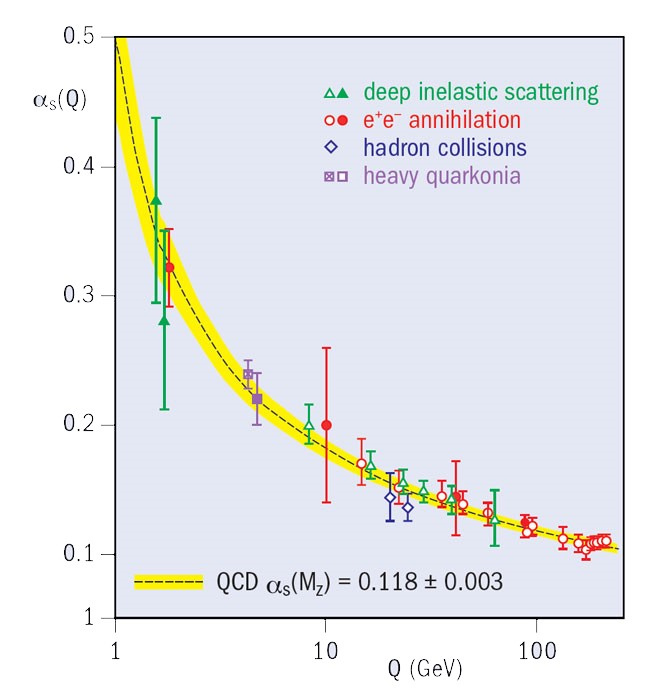
\includegraphics[width=.5\linewidth]{alpha_s.jpg}
\caption{Die Kopplungskonstante der starken Wechselwirkung $\alpha_\text{s}$ in Abh\"angigkeit des Impulsübertrags $Q$. Eingezeichnet befinden sich Messpunkte unterschiedlicher Experimente, sowie in gelb eine theoretische Rechnung.
\cite{article:1}}
\label{fig:alpha_2}
\end{figure}
Anders als die Bezeichnung vermuten l\"asst ist die Kopplungskonstante nicht konstant.
Stattdessen h\"angt $\alpha_\text{s}$ vom sogenannten Impulsübertrag $Q$ zwischen zwei Teilchen ab.
Abbildung \ref{fig:alpha_2} zeigt den Verlauf von $\alpha_\text{s}$ in Abh\"ahngigkeit von $Q$.
Der Impulsübertrag $Q$ h\"angt dabei selbst \"uber die De-Broglie-Wellenl\"ange mit dem Abstand $r$ zusammen.
Es gilt $Q = \frac{h}{\lambda}$, wobei $\lambda$ die r\"aumliche Aufl\"osung beschreibt.
F\"ur eine genau Aufl\"osung, also f\"ur  sehr kleine $r$ muss entsprechend $Q$ gro{\ss} sein.
$\alpha_\text{s}$ h\"angt also antiproportional von $r$ ab.
Aufgrund dieser Abh\"angigkeit von $\alpha_\text{s}$ bez\"uglich $Q$ beziehungsweise $r$ nennt man $\alpha_\text{s}$ auch \textit{running $\alpha_\text{s}$}. 
Den Zustand f\"ur sehr kleine $\alpha_\text{s}$ nennt man asymptotische Freiheit, da sich innerhalb dieses Zustands Quarks und Gluonen quasi frei bewegen k\"onnen.
Um so einen Zustand erzeugen zu k\"onnen braucht man eine hohe Dichte von Quarks und Gluonen oder eine hohe Temperatur.
Eine verbreitete theoretische Beschreibung eines Mediums in diesem hei{\ss}en und dichten Zustand ist das sogenannte Quark-Gluon-Plasma, kurz QGP.
\newline
Ein solcher hei{\ss}er und dichter Zustand entsteht kurz nach der Kollision von zwei hochenergetischen Atomkernen.
Quarks und Gluonen, die aus diesem Medium kommen, m\"ussen, w\"ahrend der sogenannten Hadronisierung, wieder zu Hadronen werden.
Diese Hadronen k\"onnen zerfallen, insofern sie keine stabilen Teilchen sind.
Es kann auch zu ganzen Zerfallsketten kommen, bis die Endteilchen nicht mehr zerfallen.
Je nach dem, wie schnell Teilchen zerfallen, k\"onnen entweder diese oder ihre Zerfallsprodukte gemessen werden und liefern indirekt Aufschluss auf Eigenschaften des hei{\ss}en und dichten Mediums.
\section{Proton-Proton-Kollisionen}\label{s1s3}
Neben der direkten Referenz können in der Untersuchung von pp-Kollisionen auch Informationen über die stark wechselwirkende Materie beziehungsweise über die starke Wechselwirkung selbst gewonnen werden.
pp-Kollisionen haben hierbei den Vorteil, dass sie besser theoretisch verstanden sind als Kern-Kern-Kollisionen.
Dabei führt man unter anderem die  Partonendichtefunktion der Protonen ein, die angibt, wie wahrscheinlich es ist, ein (Anti-)Quark oder Gluon mit einem bestimmten Impulsanteil des Protons vorzufinden.
Dies wiederum ermöglicht genauere theoretische Beschreibungen von pp-Kollisionen, bei denen im engeren Sinne die Partonen, also die (Anti"-)""Quarks und beziehungsweise oder Gluonen, miteinander stoßen.
\newline
Bei einem solchen Stoß entstehen viele neue Teilchen.
Die Produktionsrate der neuen Teilchen wird dabei in einem Spektrum in Abhängigkeit vom Transversalimpuls angegeben.
Der Transversalimpuls gibt dabei den Impulsanteil an, der senkrecht zur Strahlachse eines Kollisionsexperiments liegt.
Der Transversalimpuls wird deshalb betrachtet, da die kollidierenden Teilchen bei einem solchen Experiment keinen Transversalimpuls besitzen und der gesamte Transversalimpuls der entstandenen Teilchen deshalb aus den physikalischen Prozessen während und nach der Kollision kommt.
\newline
Ein mögliches Teilchen, das in Kollisionen produziert werden kann, ist das neutrale Pion.
Dieses wird in dieser Arbeit analysiert und das Spektrum des transversalen Impulses des neutralen Pions in pp-Kollisionen extrahiert.

\section{Messung neutraler Pionen zur Untersuchung des Quark-Gluon-Plasmas} \label{s1s4}
Das neutrale Pion $\pi^{0}$ besteht aus einem Quark-Antiquark-Paar und geh\"ort damit zu den Mesonen.
Genauer l\"asst sich das $\pi^{0}$ als eine \"Uberlagerung zweier quantenmechanischer Zust\"ande, bestehend aus $u$ und $d$ Quarks und den entsprechenden Antiquarks, beschreiben:
\begin{align}
\ket{\pi^{0}} = \frac{1}{\sqrt{2}}\left(\ket{u\bar{u}}-\ket{d\bar{d}}\right) \label{eq:pi0state}
\end{align}
Mit einer Masse von $m_{\pi^{0}} = \left(134,9770\pm0,0005\right) \rm{MeV}/c^{2}$ \cite{book:pdg} stellt das $\pi^{0}$ das leichteste Meson dar.
Ein ${\pi^{0}}$ zerf{\"a}llt zu $\left( 98,823\pm0,034\right)\%$ nach einer mittleren Wegl\"ange von ${\it c\tau} = (25,5\pm0,5)$nm \cite{book:pdg} in zwei Photonen.
Durch geeignete Messungen k\"onnen Energie und Position der beiden Photonen bestimmt werden.
Durch die Information \"uber die Position der Photonen kann auch der Zerfallswinkel zwischen den beiden Photonen $\theta_{\gamma\gamma}$ bestimmt werden.
Die Energien $E_{\gamma1}$ und $E_{\gamma2}$ der beiden Photonen sowie der Zerfallswinkel $\theta_{\gamma\gamma}$ werden ben\"otigt, um die invariante Masse $m_{\text{inv}}$ eines $\pi^{0}$ zu berechnen.
F{\"u}r diese gilt:
\begin{align}
m_{\text{inv}} &= \sqrt{2E_{\gamma\it{1}}E_{\gamma\it{2}}(1-\cos\left( \theta_{\gamma\gamma}\right) )} \label{eq_invmass}
\end{align}
%Die Bedeutung der invarianten Masse wird in Abschnitt \ref{s3s2} verdeutlicht.
\newline
Neben der Bestimmung der invarianten Masse kann der Impuls der Photonen aufgeteilt werden, in den Transversalimpuls und den Longitudinalimpuls.
Dabei wird in dieser Arbeit nur der Transversalimpuls $p_\text{T}$ des $\pi^{0}$ betrachtet f\"ur den gilt:
\begin{align}
p_{T\pi^{0}} &= \sqrt{\left(p_{x1}+p_{x2}\right)^{2} +\left(p_{y1}+p_{y2}\right)^{2}} \label{eq_pt}
\end{align}
Die Indizes x und y beziehen sich auf die Raumrichtungen.
\newline
Bei einem Kollisionsexperiment besitzen die beiden einfliegenden Teilchen nur einen Impuls in Strahlrichtung.
Durch Wechselwirkungen in der Kollision besitzen Teilchen, die in der Kollision entstanden sind, hingegen einen Transversalen Impulsanteil.
Daher wird oft von Teilchen, die aus der Kollision kommen, nur der transversale Impulsanteil betrachtet.
\newline
Die Messung von $\pi^{0}$ wird aus mehreren Gr\"unden zur Untersuchung von hochenergetischen Teilchenkollisionen verwendet.
\newline
Zum einen, um die Anzahl direkter Photonen bestimmen zu k\"onnen, da direkte Photonen benutzt werden k\"onnen um die Temperatur des Mediums zu bestimmen.
Als direkte Photonen werden solche Photonen bezeichnet, die in der Kollision entstehen und nicht aus Zerf\"allen stammen.
Um die Anzahl direkter Photonen bestimmen zu k\"onnen, wird die Anzahl an Zerfallsphotonen von der Gesamtzahl aller gemessenen Photonen abgezogen.
Aufgrund der hohen Zerfallswahrscheinlichkeit eines $\pi^{0}$ in zwei Photonen, sowie einer hohen Produktionsrate von $\pi^{0}$ in Teilchenkollisionen, kommt ein Gro{\ss}teil der indirekten Photonen von Zerf\"allen von $\pi^{0}$.
Deswegen wird f\"ur die Bestimmung der Anzahl direkter Photonen eine pr\"azise Messung der $\pi^{o}$ ben\"otigt.
\newline
Zum anderen wird die Anzahl produzierter $\pi^{0}$ von Kern-Kern-Kollisionen verglichen mit Kollisionen, bei denen davon ausgegangen wird, dass dort kein QGP entsteht.
Unter anderem Proton-Proton-Kollisionen werden als ein solches Vergleichssystem benutzt.
Das Verh\"altnis der Produktionsraten abh\"angig vom Transversalimpuls kann so beispielsweise Aufschluss geben auf den Energieverlust von Teilchen innerhalb des QGP.
\newline
Nachdem die theoretischen Grundlagen f\"ur die Analyse von $\pi^{0}$ dargelegt wurden, wird in Abschnitt \ref{s2} der experimentelle Aufbau n\"aher erl\"autert.

\chapter{Experimenteller Aufbau} \label{s2}
In dieser Arbeit werden Messdaten des ALICE Experiments verwendet.
Das ALICE Experiment befindet sich am LHC, den weltweit gr\"o{\ss}te Beschleunigerring, am Kernforschungszentrum CERN.
Im LHC werden Teilchen, haupts\"achlich Blei-Ionen und Protonen auf fast Lichtgeschwindigkeit beschleunigt und zum Kollidieren gebracht.
Die Beschleunigung geschieht durch elektrische Felder, w\"ahrend Dipolmagnete die beschleunigten Teilchen auf einer Kreisbahn halten.
Kollisionen finden im LHC Ring an vier unterschiedlichen Stellen statt, wo sich die Strahlrohre, in denen Teilchen gegenl\"aufig beschleunigt werden, kreuzen.
An einem dieser Punkte befindet sich das ALICE Experiment.
\newline
Die Beschleunigung auf nahezu Lichtgeschwindigkeit erm\"oglicht hohe Scherpunktsenergieen $\sqrt{s}$ zu erreichen.
Dabei spiegelt $\sqrt{s}$ die Energie wieder die das System in einer Kollision zur Verf\"ugung hat.
Dementsprechend k\"onnen mehr und auch schwerere Teilchen bei h\"oherem $\sqrt{s}$  in einer Kollision entstehen.
Ein hohes $\sqrt{s}$ hat auch eine h\"ohere Temperatur des Mediums was bei einer solchen Kollision entstehen kann zur Folge.
So befinden sich Messungen des ALICE Experiments am LHC im Phasendiagramm stark wechselwirkender Materie, wie es in Abbildung \ref{fig:QGPPhase} skizziert ist, bei hohen Temperaturen und einer geringen Baryonendichte.
$\sqrt{s}$ h\"angt dabei von der Energie der kollidierende Teilchen ab.
F\"ur Kollisionsexperimente zweier identischer Teilchen mit gleicher Energie $E$ gilt:
\begin{align}
\sqrt{s} = 2E \label{eq:sqrts}
\end{align}
\newline
Im folgenden Abschnitt wird das ALICE Experiment genauer beschrieben.
\section{ALICE} \label{s2s1}
Das ALICE Experiment wurde speziell zur Untersuchung des Quark-Gluonen-Plasmas konzipiert und gebaut.
Um die Anspr\"uche daf\"ur besonders gut erf\"ullen zu k\"onnen besteht das ALICE Experiment aus einer Vielzahl unterschiedlicher Detektoren.
\begin{figure}[thp]
\centering
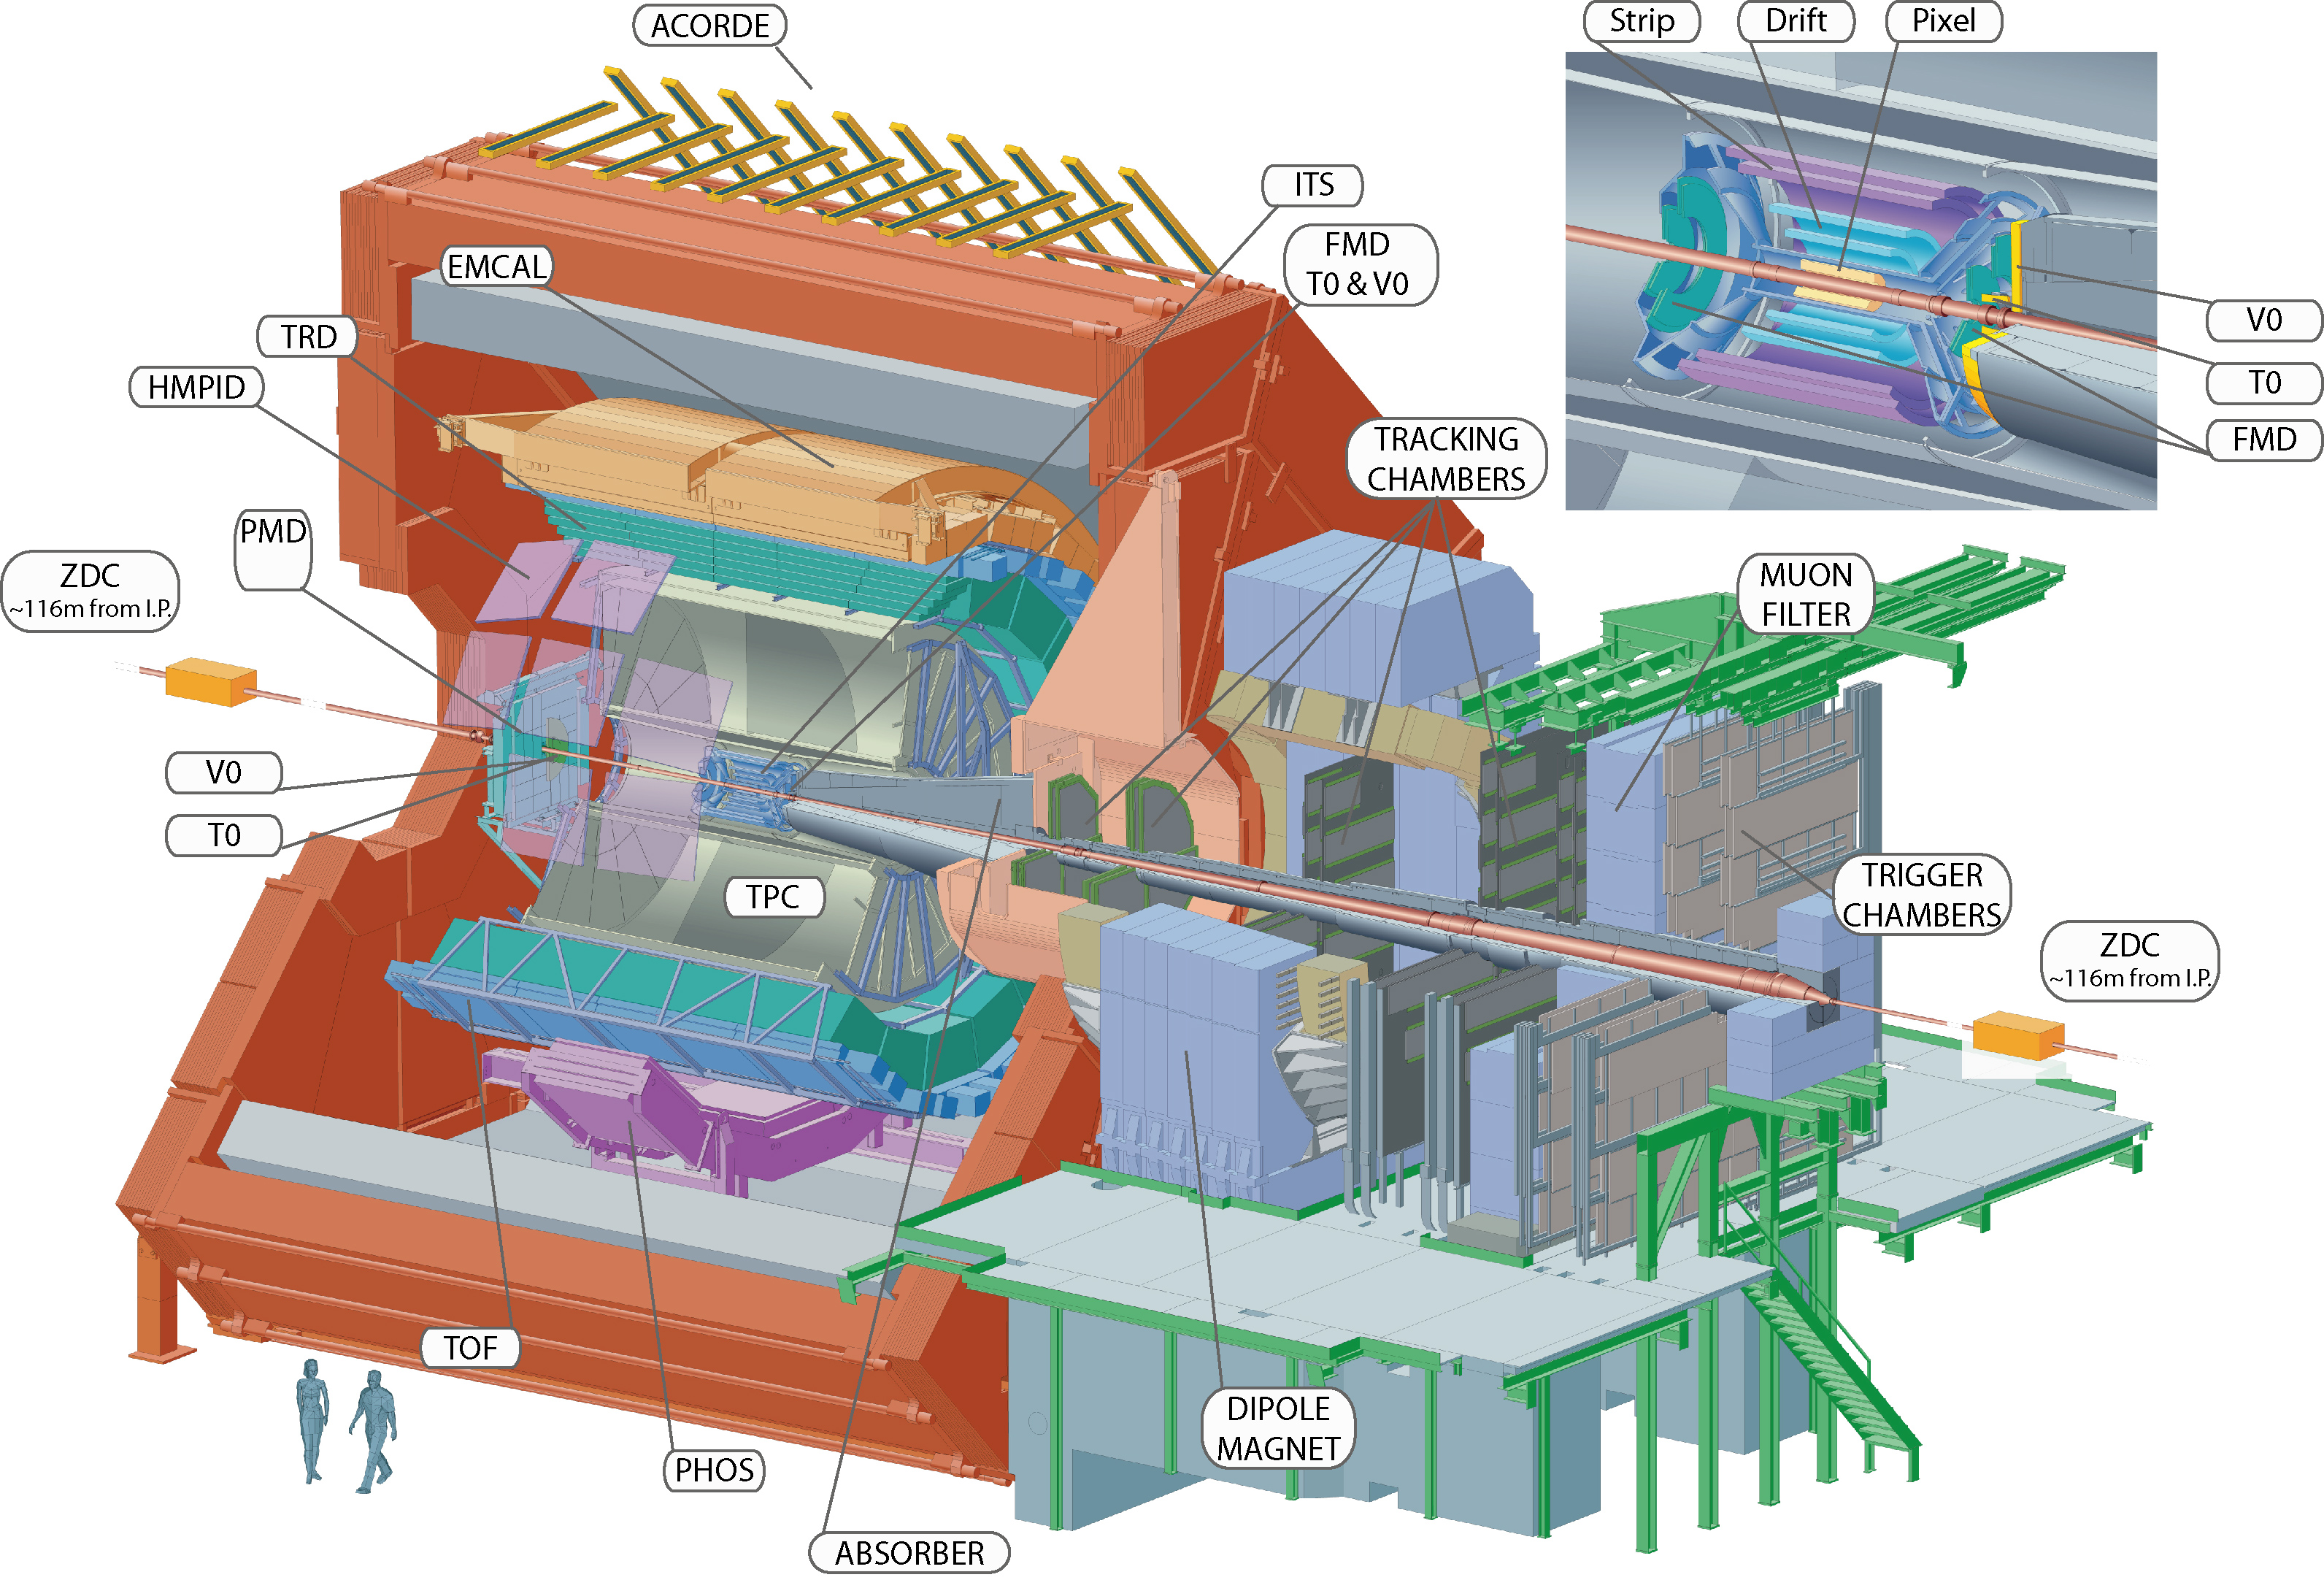
\includegraphics[width=.9\linewidth]{ALICE.jpg}
\caption{Schematische Darstellung des Querschnitts des ALICE Experiments.
\cite{WEBSITE:1}}
\label{fig:ALICE}
\end{figure}
Abbildung \ref{fig:ALICE} zeigt schematisch einen Querschnitt des ALICE Experiments. Der zylinderf\"ormige Aufbau um das Kollisionszentrum ist typisch f\"ur Kollisionsexperimente.
\newline
Um die zentralen Detektoren befindet sich ein gro{\ss}er roter Solenoid-Magnet, der ein Magnetfeld von 0,5 T erzeugt, wodurch geladene Teilchen auf gekr\"ummte Flugbahnen gelenkt werden.
Mit Hilfe der Radien k\"onnen einige der geladenen Teilchen identifiziert werden.
Im Folgenden werden die f\"ur diese Analyse wichtigsten Detektoren kurz eingef\"uhrt.
\newline
\textbf{Inner Tracking System}
\newline
Das Inner Trackign System, kurz ITS, befindet sich im innersten des ALICE Experiments und besteht aus sechs Schichten.
Von innen nach au{\ss}en au{\ss}en sind die Schichten zwei Silicon Pixel Detectors, kurz SPD, zwei Silicon Drift Detectors, kurz SDD, und zwei Silicon Strip Detectors, kurz SSD.
Das ITS wird haupts\"achlich zur Ortsbestimmung des sogenannten prim\"aren Vertex benutzt.
Der prim\"are Vertex ist die Absch\"atzung des Kollisionspunktes.
\newline
\textbf{Time Projection Chamber}
\newline
Die Time Projection Chamber, kurz TPC, umschlie{\ss}t das ITS und dient als zylinderf\"ormiger Detektor der Spurrekonstruktion.
Die TPC ist mit Gas gef\"ullt und hat an beiden Enden jeweils eine Hochspannungselektrode, wodurch zwei gegens\"atzliche elektrische Felder im inneren der TPC vorliegen.
Fliegen geladene Teilchen durch die TPC, so ionisieren die geladenen Teilchen das Gas.
Das ionisierte Gas wiederum wird durch das elektrische Feld in Richtung der Endplatten beschleunigt, an denen sich auch Ausleseelektronik befindet.
Durch die Bahnkr\"ummung, sowie der Dichte der Gasionisation von den geladenen Teilchen k\"onnen die geladenen Teilchen identifiziert werden. \cite{PAPER:2}
\newline
\textbf{V0-Detektoren}
\newline
Die sogenannte V0-Detektoren bestehen aus zwei einzelnen Detektoren, welche sich jeweils an einem Ende des ITS um die Strahlenachse befinden.
Messen beide V0 Detektoren eine bestimmte Mindestanzahl an Teilchen, so wird die Aufzeichnung einer Kollision (engl. \textit{Event}) gestartet.
Solche Anforderungen werden allgemein als \textit{trigger} bezeichnet, diese Anforderung, dass die V0-Detektoren eine Mindestanzahl an Teilchen detektieren m\"ussen, nennt man entsprechend \textit{minimum-bias trigger}.
\newline
\textbf{T0-Detekroren}
\newline
Genauso wie die V0-Detekroren bestehen die T0-Detektoren auch aus zwei einzelnen Detektoren, welche sich ebenfalls an den Enden der ITS befinden.
Bei den T0-Detektoren handelt es sich um pr\"azise Zeitdetektoren, die der genauen Bestimmung des Kollisionszeitpunkts dienen.
\newline
\textbf{Elektromagnetische Kaloriemeter}
\newline
Das elektromagnetische Kaloriemeter, kurz EMCal, befindet sich am \"au{\ss}ersten Rand des zentralen Detektorkomplexes.
Aufgrund der Wichtigkeit des EMCals f\"ur diese Analyse wird das EMCal im folgenden Abschnitt genauer erl\"autert.
\section{Elektromagnetische Kaloriemeter EMCal} \label{s2s2}
Der Hauptdetektor dieser Analyse ist das EMCal.
In einem Abstand von 4,5m vom prim\"aren Vertex deckt das EMCal einen Azimuthalwinkelbereich von $\phi=107^{\circ}$ und einen Rapidit\"atsbreich von $ |\eta| \leq 0,7$ ab.
Aufgrund von Detektormaterial und Tr\"agerstrukturen zwischen dem prim\"aren Vertex und dem EMCal k\"onnen Teilchen abgelenkt werden oder Photonen in ein Elektron-Positron-Paar konvertieren.
Die Konvertierung von Photonen ist besonders zu beachten, da in dieser Analyse $\pi^{0}$, welche in zwei Photonen zerfallen, rekonstruiert werden.
\newline
Das EMCal besteht aus zw\"olf sogenannten Supermodulen, zehn normal gro{\ss}e und zwei Eindrittel gro{\ss}e.
Ein normal gro{\ss}es Supermodul unterteilt sich in 24 sogenannte Streifenmodule, welche wiederum aus 12 Modulen zusammengesetzt sind.
Jedes Modul beinhaltet 4 Zellen, womit das EMCal aus insgesamt 12288 Zellen besteht.
Die Zellen sind f\"ur das Detektieren und Messen der Energie von haupts\"achlich Photonen, Elektronen und Positronen verantwortlich.
Daf\"ur besteht eine einzelne Zelle aus abwechselnd 77 Szintillatoren- und 76 Bleischichten.
In den Bleischichten entstehen sogenannten elektromagnetische Schauer, indem eintreffende Photonen durch Paarerzeugung in ein Elektron und ein Positron zerfallen, welche wiederum durch Bremsstrahlung weitere Photonen abstrahlen.
Die Szintillatoren wandeln die hochenergetischen Photonen in ein messbares Lichtsignal.
Alle Szintillatorschichten einer Zelle sind \"uber ein Glasfaserkabel mit einem Photomultiplier verbunden.
Der Photomultiplier wandelt das Lichtsignal in ein elektrisches Signal, welches proportional zu gespeicherten Energie der Zelle ist.
\newline
Jeder elektromagnetischer Schauer besitzt eine gewisse Ausdehnung, welche \"uber den sogenannten Moli\`ere-Radius $R_{\text{M}}$ definiert ist.
Der Moli\`ere-Radius gibt den Radius passend zu einem Zylinder an, in welchem 90\% der gesamten Energie eines Schauers vom Detektor absorbiert wurde.
F\"ur das EMCal betr\"agt der Moli\`ere-Radius $R_{\text{M}} = 3,7 cm$, womit sich eine Kreisfl\"ache von ca. $43 cm^{2}$ ergibt.
Die einzelnen Zellen des EMCal hingegen haben eine quadratische Fl\"ache von $36 cm^{2}$. 
Der Schauer eines einzelnen Teilchens erstreckt sich also \"uber mehrere Zellen, weshalb mehrere Zellen durch eine Algorithmus zu sogenannten \textit{Clustern} zusammengefasst werden.
Algorithmen zur Rekonstruktion von \textit{Clustern} hei{\ss}en \textit{Clusterizer}.
In der hier vorliegenden Analyse wird der sogenannte v2-\textit{Clusterizer} verwendet.
Dieser sucht zun\"achst nach der Zelle mit der gr\"o{\ss}ten deponierten Energie, welche noch keinem \textit{Cluster} angeh\"ohrt und eine gewisse Schwellenenergie besitzt.
Von dieser Startzelle ausgehend werden die Nachbarzellen abgesucht und zum \textit{Cluster} hinzugef\"ugt, wenn sie eine gewisse Mindestenergie \"uberschreiten und ebefalls keinem weiteren \textit{Cluster} zugeordnet sind.
Dies Suche nach Nachbarzellen geschieht dabei iterativ solange, bis keine Nachbarzellen die n\"otigen Kriterien erf\"ullen um dem \textit{Cluster} hinzugef\"ugt zu werden.
Anschlie{\ss}end wird eine neue Startzelle f\"ur ein neues \textit{Cluster} gesucht und der Prozess beginnt von vorne.

\begin{figure}[thp]
\centering
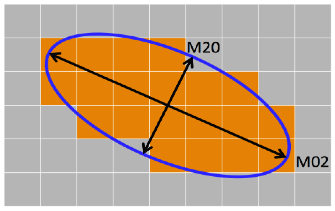
\includegraphics[width=.35\linewidth]{m02&m20.png}
\caption{Schematische Darstellung eines \textit{Clusters}. Die Ellipsenhalbachsen M20 und M02 definieren eine Ellipse, welche alle orange markierten Zellen, die zu einem \textit{Cluster} geh\"ohren, umfasst.
[Masterarbeit Adrian oder bearbeiten]}
\label{fig:M20}
\end{figure}

Abbildung \ref{fig:M20} zeigt eine schematische Darstellung eines \textit{Clusters}.
Alle orange eingef\"arbten Zellen geh\"oren dabei zu einem \textit{Cluster}.
Die eingezeichnete Ellipse, beziehungsweise ihre Halbachsen M02 und M20, helfen dabei das \textit{Cluster} zu parametrisieren.
Die Form eines \textit{Clusters} und damit die gr\"o{\ss}e von M02 und M20 unterscheidet sich abh\"angig davon, ob das \textit{Cluster} durch ein Hadron entstanden ist oder nicht.
Dadurch kann M02 benutzt werden um \textit{Cluster} welche nicht durch Hadronen entstanden sind zu identifizieren.
Die Teilchen die zu diesen \textit{Clustern} geh\"oren werden im Weiteren als Photonenkandidaten bezeichnet.
F\"ur M02 gilt:
\begin{align} 
M_{02} = \frac{1}{2}\sum_{i}E_{i}(x_{i}^{2}+y_{i}^{2})+\sqrt{\frac{1}{4}\sum_{i}\left(x_{i}^{2}+y_{i}^{2}\right)^{2}+\left(\sum_{i}E_{i}x_{i}y_{i}\right)}
\end{align}
Wobei $E_{i}$ f\"ur die Energie einer Zelle und $x_{i}$ und $y_{i}$ f\"ur die relative Position einer Zelle zur Startzelle steht.

\chapter{Messung neutraler Pionen mit Hilfe des EMCal} \label{s3}

\section{Datenauswahl} \label{s3s1}

\subsection{Datensatz} \label{s3s1s1}
In dieser Arbeit werden Daten von pp-Kollisionen bei $\sqrt{s}=13\text{ TeV}$ verwendet, die mit dem ALICE Experiment gemessen wurden.
Die Datensätze werden unterteilt in Perioden, die ungefähr einem Monat Aufnahmezeit entsprechen.
Dabei existiert eine Namenskonvention für die Perioden.
Sie beginnen immer mit LHC, gefolgt von den zwei hinteren Jahreszahlen in der die Periode gemessen wurde.
Zuletzt noch ein Kleinbuchstabe der die Perioden sortiert, beginnend bei a.
Die Perioden die in dieser Analyse verwendet werden sind $LHC16h\,i\,j\,k\,l$.
Diese umfassen circa 250 Millionen \textit{minimum-bias events}.
\newline
Für die Monte Carlo Simulation wurde der Ereignisgenerator PYTHIA 8 mit dem \textit{tune} Monash 2013 benutzt.
Dabei sei erneut auf \cite{thesis:Krissy} verwiesen.
Außerdem wurde GEANT3 verwendet um die möglichen Interaktionen mit dem ALICE Experiment zu simulieren \cite{Brun:118715}.
Die Monte Carlo Simulation wurde dabei an die  Perioden $LHC16h\,i\,j\,k\,l$ angepasst.
Insgesamt umfasst die Monte Carlo Simulation etwa 280 Millionen \textit{minimum-bias events}.

\subsection{Clusterauswahlkriterien} \label{s3s1s2}
An die mit dem EMCal aufgenommenen \textit{Cluster} aus dem gewählten Datensatz werden unterschiedliche Anforderungen gestellt.
Tabelle \ref{tab:Cluster} listet die in dieser Analyse gestellten Anforderungen auf.
\begin{table}[b]
\centering
\begin{tabular}{|l|r|}
\hline
\multicolumn{2}{|c|}{Clusterauswahlkriterien}                   \\ \hline \hline
Zeit                    & $-30\text{ ns} < t_\text{clust}<35\text{ ns}$ \\ \hline
\textit{Bad Cell Map}   & angewandt                                     \\ \hline
Energie                 & $E_\text{clust}\geq700\text{ MeV}$                         \\ \hline
Anzahl Zellen           & $N_\text{Zellen}\geq 2$                       \\ \hline
Form                    & $0.1< M_{02}<0.7$                             \\ \hline
\textit{Track Matching} & $p_\text{T}$ abhängig: $\Delta\eta$ $\Delta\phi$                                     \\ \hline
Öffnungswinkel          & $\theta>0.017\text{ rad}$                     \\ \hline
\end{tabular}
\caption{Auswahlkriterien für die \textit{Cluster} des EMCals.}
\label{tab:Cluster}
\end{table}
\newline
Der zeitliche Rahmen, in dem die \textit{Cluster} entstanden sind, wird um den Kollisionszeitpunkt ein\-ge\-schränkt, um \textit{Cluster} von Teilchen auszuschließen, die nicht von einem \textit{Event} stammen.
Die \textit{Bad Cell Map} wird verwendet, um schlechte Zellen von der Analyse auszuschließen \cite{thesis:Joshua}.
\newline
Die Energie, die ein \textit{Cluster} mindestens braucht, sowie die Anforderung an die Form und die Anzahl an Zellen, aus denen ein \textit{Cluster} mindestens bestehen muss, helfen \textit{Cluster} von Photonen zu selektieren.
Die Mindestenergie von $700\text{ MeV}$ wir benötigt um detektorbedingtes  Rauschen zu unterdrücken.
Der Schwellenwert für die Energie steht dabei im direkten Zusammenhang mit der Mindestanzahl an Zellen.
Wie in Abschnitt \ref{s2s2} erwähnt, benötigt die Startzelle eine deponierte Energie von mindestens 600 MeV und jede weitere Zelle von mindestens 100 MeV, um zu einem \textit{Cluster} hinzugefügt zu werden.
Um die angegebene Mindestenergie zu erreichen benötigt ein \textit{Cluster} entsprechend mindestens zwei Zellen.
Die Form, charakterisiert durch den Parameter $M_{02}$, wurde in Abschnitt \ref{s2s2} bereits erläutert.
Mit Hilfe des \textit{Track Matching} können \textit{Cluster}, die von geladenen Teilchen kommen, ausgeschlossen werden, um die Reinheit des Signals zu erhöhen.
Dafür werden die Spuren der geladenen Teilchen, die in der TPC hinterlassen wurden, rekonstruiert und bis zum EMCal extrapoliert.
Einige Photonen konvertieren erst nach dem sie die TPC passiert haben.
\textit{Cluster} durch Elektronen beziehungsweise Positronen aus diesen Konversionen können entsprechend nicht durch das \textit{Track Matching} ausgeschlossen werden. 
\newpage
\noindent
Durch die Anforderung an den Öffnungswinkel wird sicher gestellt, dass der Abstand zwischen zwei \textit{Clustern} mindestens der Größe einer Zellendiagonale entspricht.
Diese Anforderung wird für die Bestimmung des Untergrunds benötigt.

\section{Clusterkombination} \label{s3s2}
Die gewählten \textit{Cluster} nach den Kriterien aus Abschnitt \ref{s3s1s2} bestehen fast ausschließlich aus Photonen, und  Elektronen beziehungsweise Positronen aus der Konversion eines Photons.
\begin{figure}[t!]
\centering
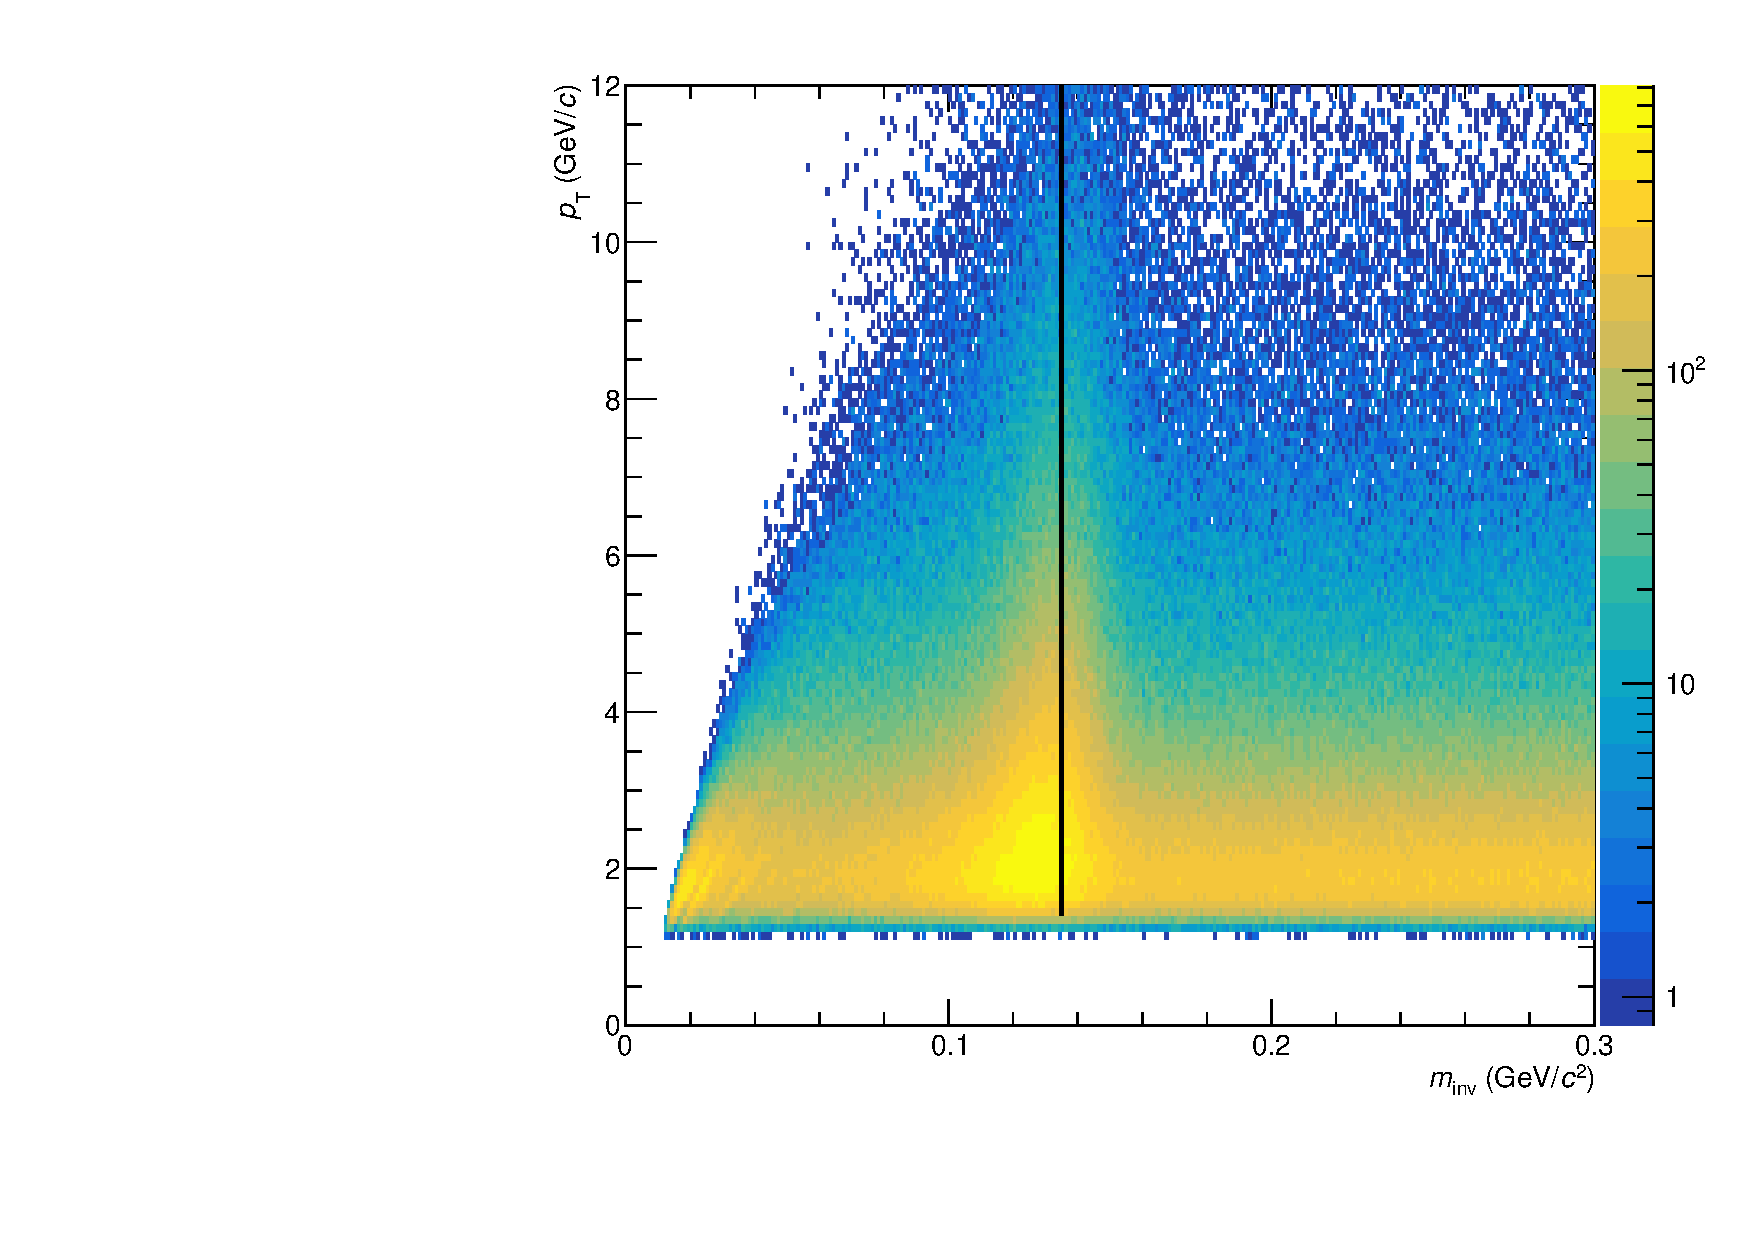
\includegraphics[width=.7\linewidth]{hInvMass_pT_Signal.pdf}
\caption{$p_\text{T}$ und $m_\text{inv}$ als Funktion der Anzahl von kombinierten  Cluster-Paaren aus der gleichen Kollision.
Die rote Linie liegt bei $m_{\text{inv}}\approx0\,135\text{ GeV/}c^{2}$, was in etwa der $\pi^{0}$ Masse entspricht, wo eine deutliche Häufung der Einträge sich abzeichnet.
Die schwarzen Linien stellen die Grenzen der $p_{\text{T}}$-Intervalle dar.}
\label{figInvMassPt_a}
\end{figure}
\newline
Um die Anzahl der detektierten $\pi^{0}$ zu messen, werden von \textit{Clusterpaaren} die invariante Masse und der Transversalimpuls nach Gleichungen \ref{eq_invmass} und \ref{eq_pt} bestimmt.
Da die Information fehlt, ob und welche \textit{Cluster} von einem Teilchen aus dem Zerfall eines $\pi^{0}$ stammen, werden alle \textit{Cluster} eines \textit{events} paarweise mit einander kombiniert.
Diese Methode wird als \textit{same event} Methode bezeichnet.
Abbildung \ref{figInvMassPt_a} zeigt die Anzahl der \textit{Clusterpaare} in Abhängigkeit der invarianten Masse $m_{\text{inv}}$ und des Transversalimpulses $p_{\text{T}}$.
Durch die paarweise Kombination aller \textit{Cluster} eines \textit{Events} gibt es sowohl Kombinationen von \textit{Cluster} von Teilchen die aus dem Zerfall eines $\pi^{0}$ stammen, als auch \textit{Cluster} von Teilchen die nicht über den Zerfall eines einzelnen $\pi^{0}$ zusammenhängen.
\newline
Die Summe aller \textit{Clusterpaare}, die aus einem Zerfall eines $\pi^{0}$ kommen, wird als Signal bezeichnet.
Es zeichnet sich eine Häufung der Datenpunkte um $m_{\text{inv}}\approx 0\,135\text{ GeV}/c^{2}$, also um die Masse des $\pi^{0}$, ab.
Dieser Häufung liegt vor allem das Signal zugrunde.
Da Photonen durch Paarbildung in ein Elektron und ein Positron konvertieren können, bestehen einige\textit{Cluster} aus nur einem der beiden Konversionsprodukte.
Diese \textit{Cluster} besitzen eine geringere Energie, als das eigentliche Photon besaß.
Durch Kombinationen dieser \textit{Cluster} entstehen Einträge bei einer invarianten Masse, die meistens geringer ist als die Masse von $\pi^{0}$, wenn beide Teilchen, die dem \textit{Cluster} zugrunde liegen, dem selben $\pi^{0}$ entstammen.
Deshalb wird bei invarianten Massen $m_\text{inv}<0\,135\text{ GeV}/c^{2}$ ein Teil des Signals erwartet.
\newline
Alle \textit{Clusterpaare}, die nicht zum Signal zählen, bilden den Untergrund, der in zwei Teile unterteilt wird, dem kombinatorischen oder auch unkorrelierten Untergrund und dem korrelierten Untergrund.
Dem korrelierten Untergrund liegen paarweise Kombinationen von \textit{Cluster} zugrunde, zwischen denen eine Korrelation besteht.
Das heißt, dass die Teilchen der zugehörigen \textit{Cluster}, nicht aus dem Zerfall eines einzelnen $\pi^{0}$ stammen, aber über andere Zerfälle zusammenhängen.
Durch die paarweise Kombination von \textit{Cluster} von unkorrelierter Teilchen entsteht der unkorrelierte Untergrund.
\newline
Aufgrund der Anforderung an den Öffnungswinkel werden stetig mehr Kombinationsmöglichkeiten der \textit{Cluster} ausgeschlossen, da ein immer  größerer Anteil der \textit{Cluster} aus zwei Teilchen besteht.
Die ausgeschlossenen Kombinationen liegen im Bereich kleiner invarianter Massen weshalb es bei bei kleinem $m_{\text{inv}}$ keine Datenpunkte gibt.
Das führt dazu, dass mit steigendem $p_{\text{T}}$ immer mehr Signal nicht rekonstruierbar wird.
\newline
Die Anzahl der $\pi^{0}$ weist eine $p_{\text{T}}$-Abhängigkeit auf.
Deshalb wird die Verteilung aus Abbildung \ref{figInvMassPt_a} in einzelnen $p_{\text{T}}$-Intervallen analysiert.
Die Intervalle werden so gewählt, dass sie möglichst klein sind, während die statistischen Unsicherheiten der Datenpunkte nicht zu groß werden.
\begin{figure}[tbp]
\centering
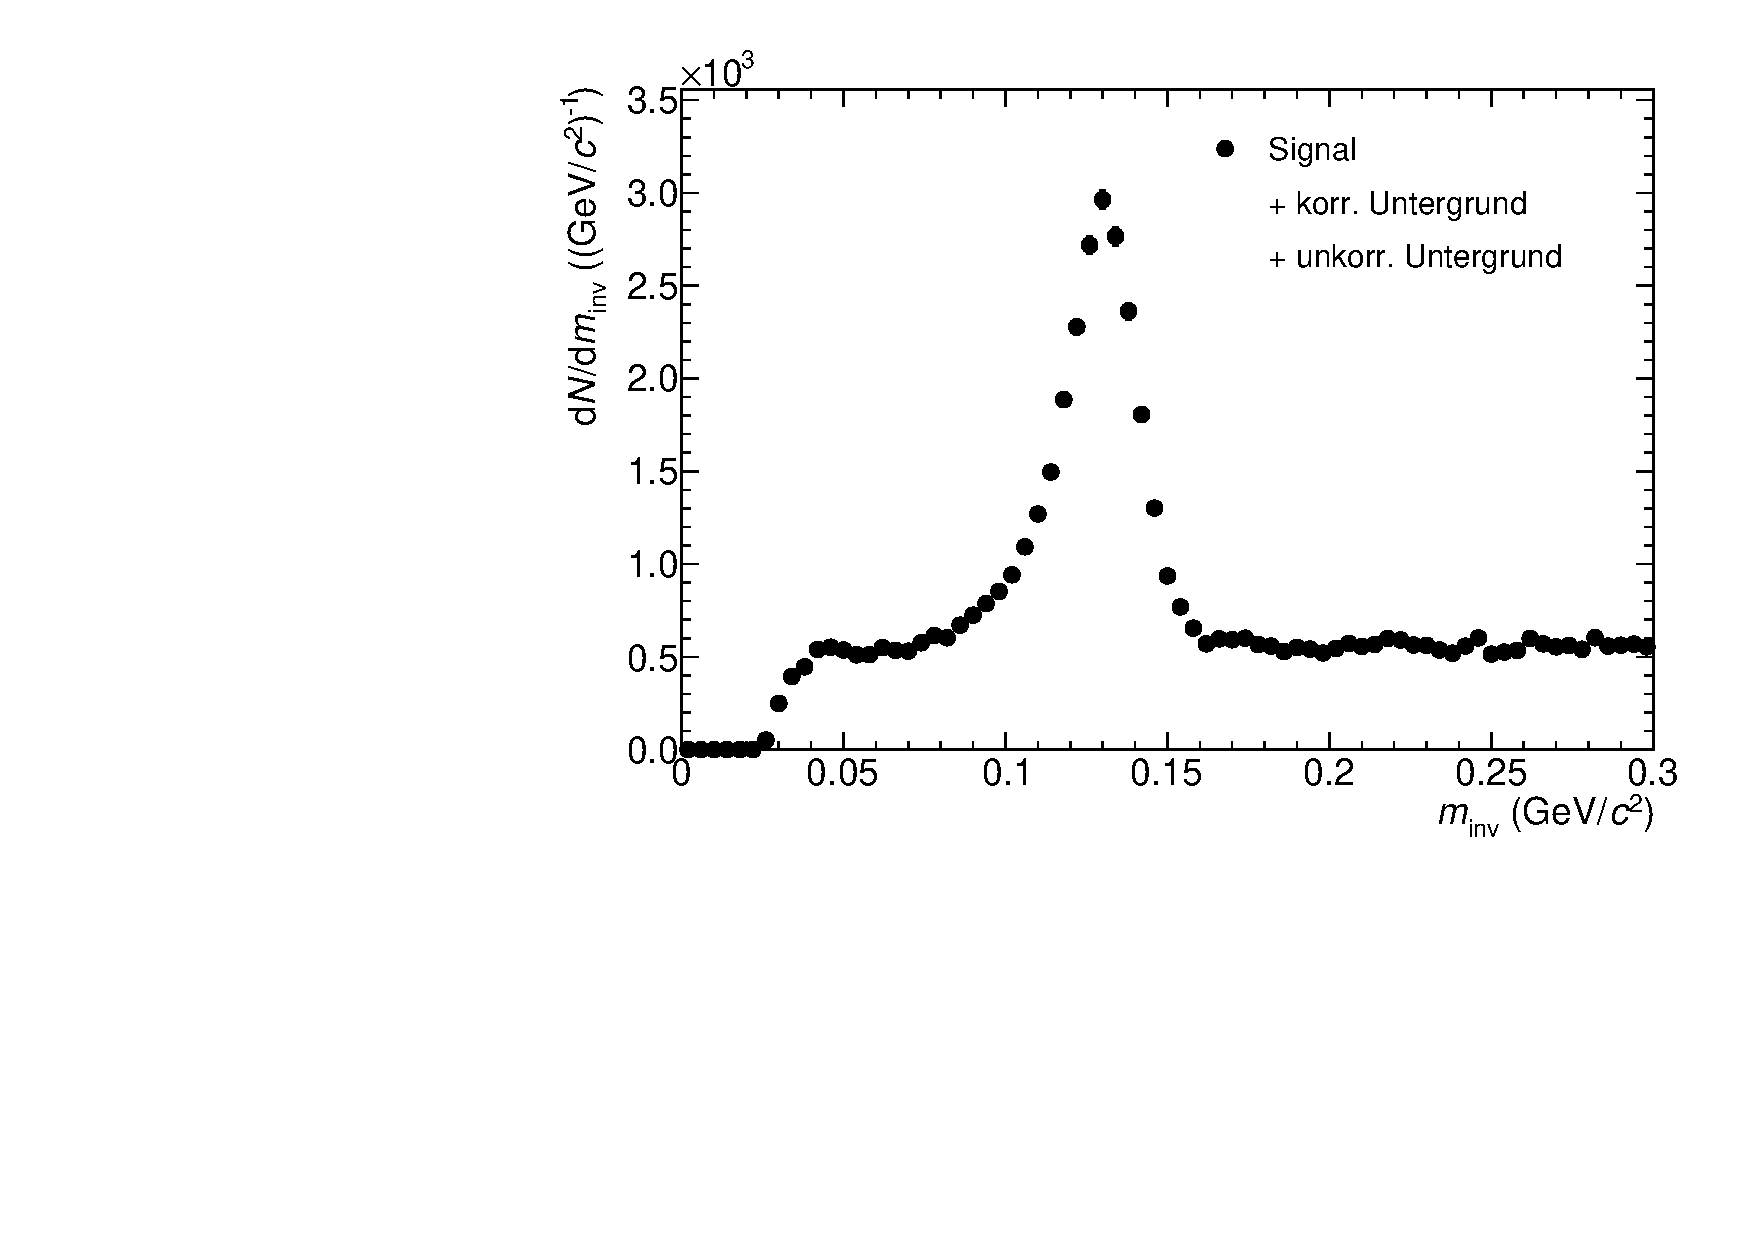
\includegraphics[width=.75\linewidth]{hSignalPlusBkg.pdf}
\caption{Projektion von Abbildung \ref{figInvMassPt_a} im $p_{\text{T}}$-Intervall $(3,2 - 3,4) (\text{GeV/}c)$. Es ist ein deutlicher Peak um $m_{\pi^{0}} \approx 0\,135\text{ GeV/}c^{2}$ zu erkennen, aber auch Untergrund, da das Signal zu höheren Massen gaußförmig abklingen sollte. Bei $m_{\text{inv}} < m_{\pi^{0}}$ kann Signal vorliegen, das aus konvertierten Photonen besteht, weshalb eine Aussage über die Form, beziehungsweise den Untergrund dort schwer möglich ist.}
\label{figSignalPlusBkg}
\end{figure}
\newline
Abbildung \ref{figSignalPlusBkg} zeigt die Anzahl der \textit{Clusterpaare} in Abhängigkeit der invariante Massen im $p_{\text{T}}$-Intervall von $(3\,2 - 3\,4)(\text{GeV}/c)$.
Die in Abbildung \ref{figInvMassPt_a} beschriebene Anhäufung der Datenpunkten zeigt sich auch hier deutlich und wird im Folgenden als Peak bezeichnet.
Der Peak besteht wie zuvor erwähnt hauptsächlich aus Signal.
\newline
Im folgenden Abschnitt wird eine Methode zur Abschätzung des unkorrelierten Untergrunds vorgestellt. 

\section{Absch{\"a}tzung des unkorrelierten Untergrunds} \label{s3s3}
\begin{figure}[tp]
\centering
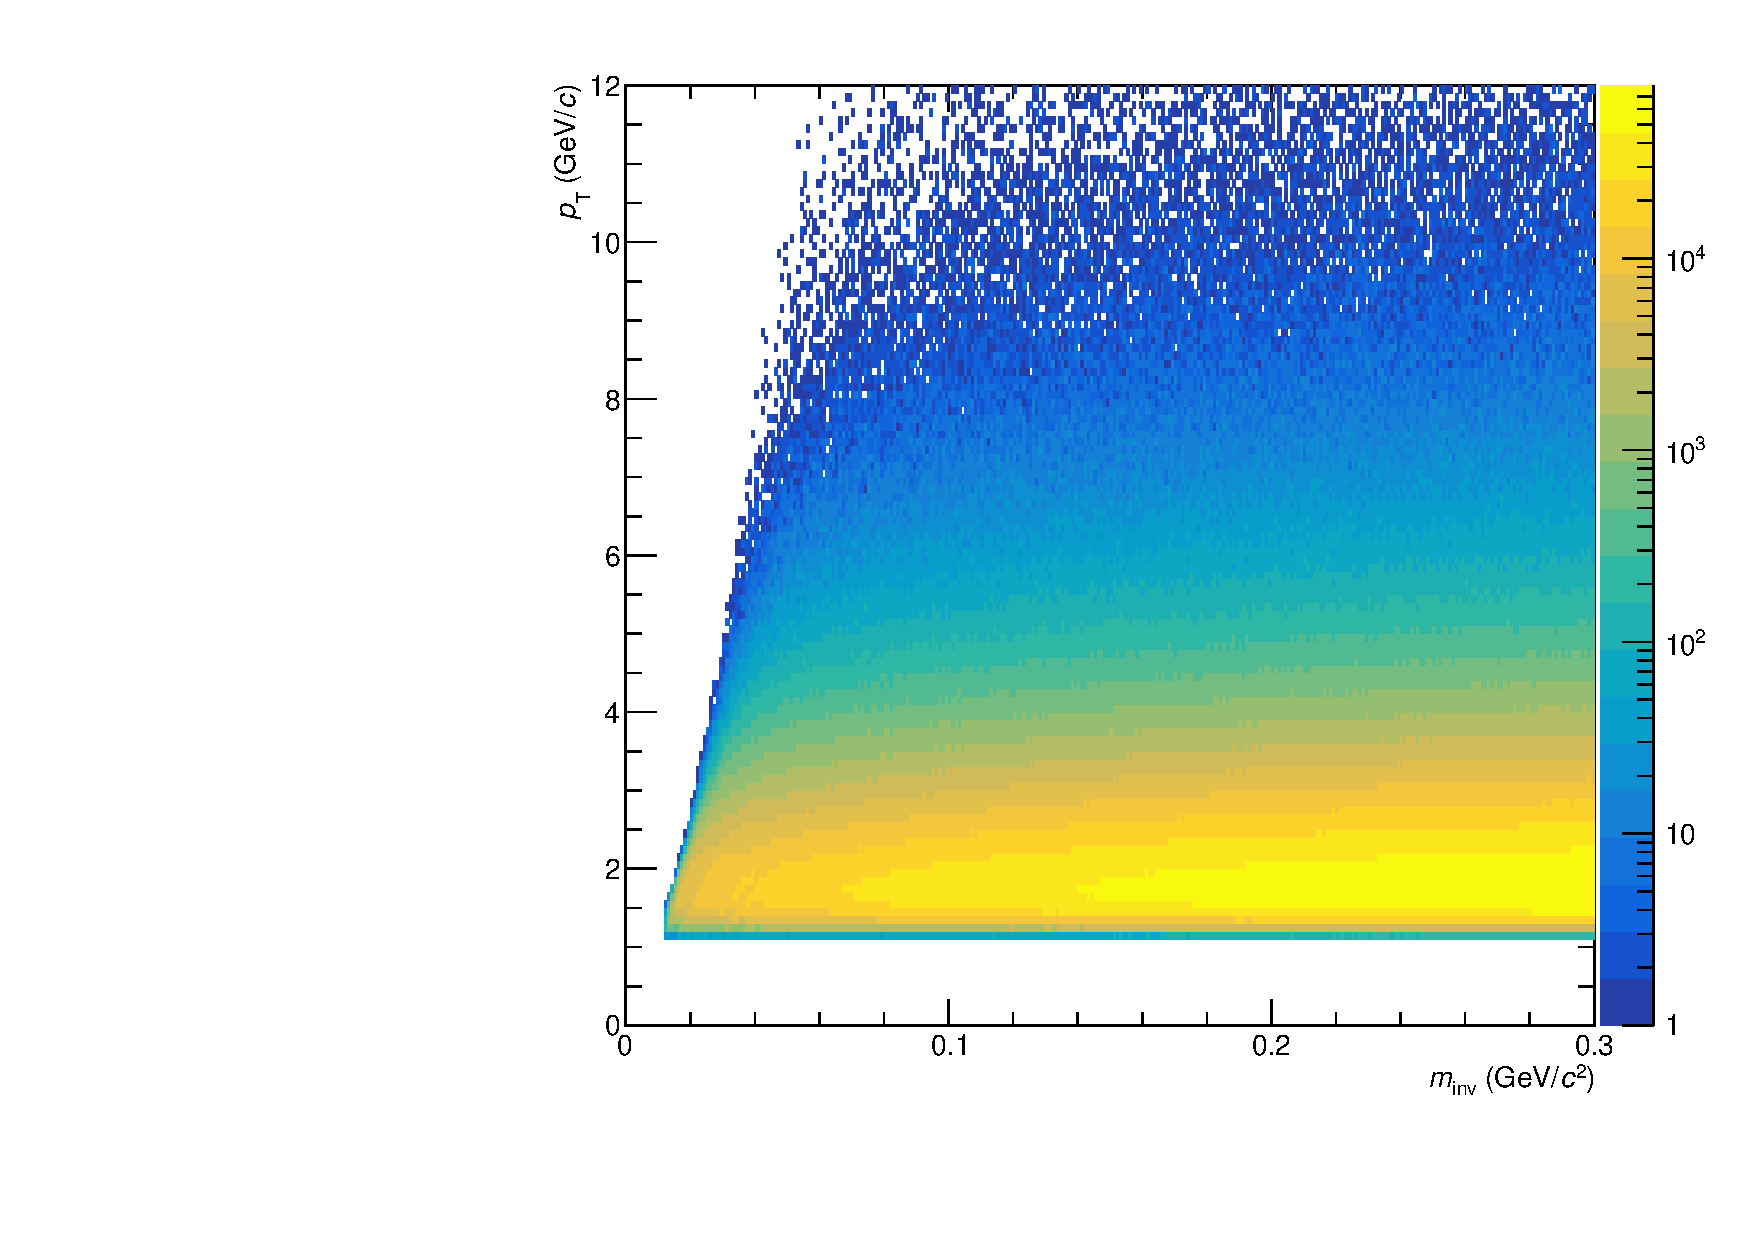
\includegraphics[width=.7\linewidth]{hInvMass_pT_Bkg.pdf}
\caption{$p_\text{T}$ und $m_\text{inv}$ als Funktion von der Anzahl von kombinierten  \textit{Clusterpaaren} aus unterschiedlichen \textit{events}.}
\label{figInvMassPt_b}
\end{figure}
Durch das paarweise Kombinieren aller Photonenkandidaten, wie es in Abschnitt \ref{s3s2} vorgestellt wurde, besteht ein großer Anteil der rekonstruierten Datenpunkte aus unkorreliert Paaren.
Um den unkorrelierten Untergrund abzuschätzen werden Photonenkandidaten aus unterschiedlichen \textit{events} paarweise miteinander kombiniert.
Diese Methode wird als \textit{mixed event} Methode bezeichnet.
Abbildung \ref{figInvMassPt_b} zeigt eine Verteilung, bei der Photonenkandidaten aus unterschiedlichen \textit{events} miteinander kombiniert wurden.
Eine Häufung der Datenpunkte um eine bestimmte invariante Masse gibt es, wie zu erwarten, nicht.
Durch die Anforderungen an den Öffnungswinkel sind wieder keine Datenpunkte bei kleinen invarianten Massen zu finden.
Die untere Grenze, ab welcher invarianten Masse Kombinationen möglich sind steigt mit $p_\text{T}$, analog wie zuvor bei Abbildung  \ref{figInvMassPt_a}.
\newline
In der \textit{mixed event} Methode gibt es eine größere Anzahl an Kombinationsmöglichkeiten, als in der \textit{same event} Methode.
Daraus resultiert eine größere Anzahl an Einträgen in der Verteilung der invarianten Masse und des Transversalimpulses, weshalb die Verteilung, die aus der \textit{mixed event} Methode kommt, skaliert werden muss an die Verteilung aus der \textit{same event} Methode.
Die Skalierung erfolgt bei $m_\text{inv} \in \left[0\,19,3\,0\right] (\text{GeV/}c^{2})$, da dort kein Signal erwartet wird.
Es ergibt sich für den Skalierungsfaktor:
\begin{align}
\label{eqBackSkalierung}
\alpha &= \frac{\sum_{i \neq j}\sum_{n}m_{\text{inv}}\left( \gamma^{(n)}_{i},\gamma^{(n)}_{j}\right) }{\sum_{i,j}\sum_{n \neq m}m_{\text{inv}}\left( \gamma^{(n)}_{i},\gamma^{(m)}_{j}\right) }
\end{align}
Die oberen Indize $m$ und $n$ stehen hierbei für ein Event, aus dem ein Photon kommt und die unteren Indize $i$ und $j$ numerieren die Photonen ($\gamma$).
\begin{figure}[tp]
\centering
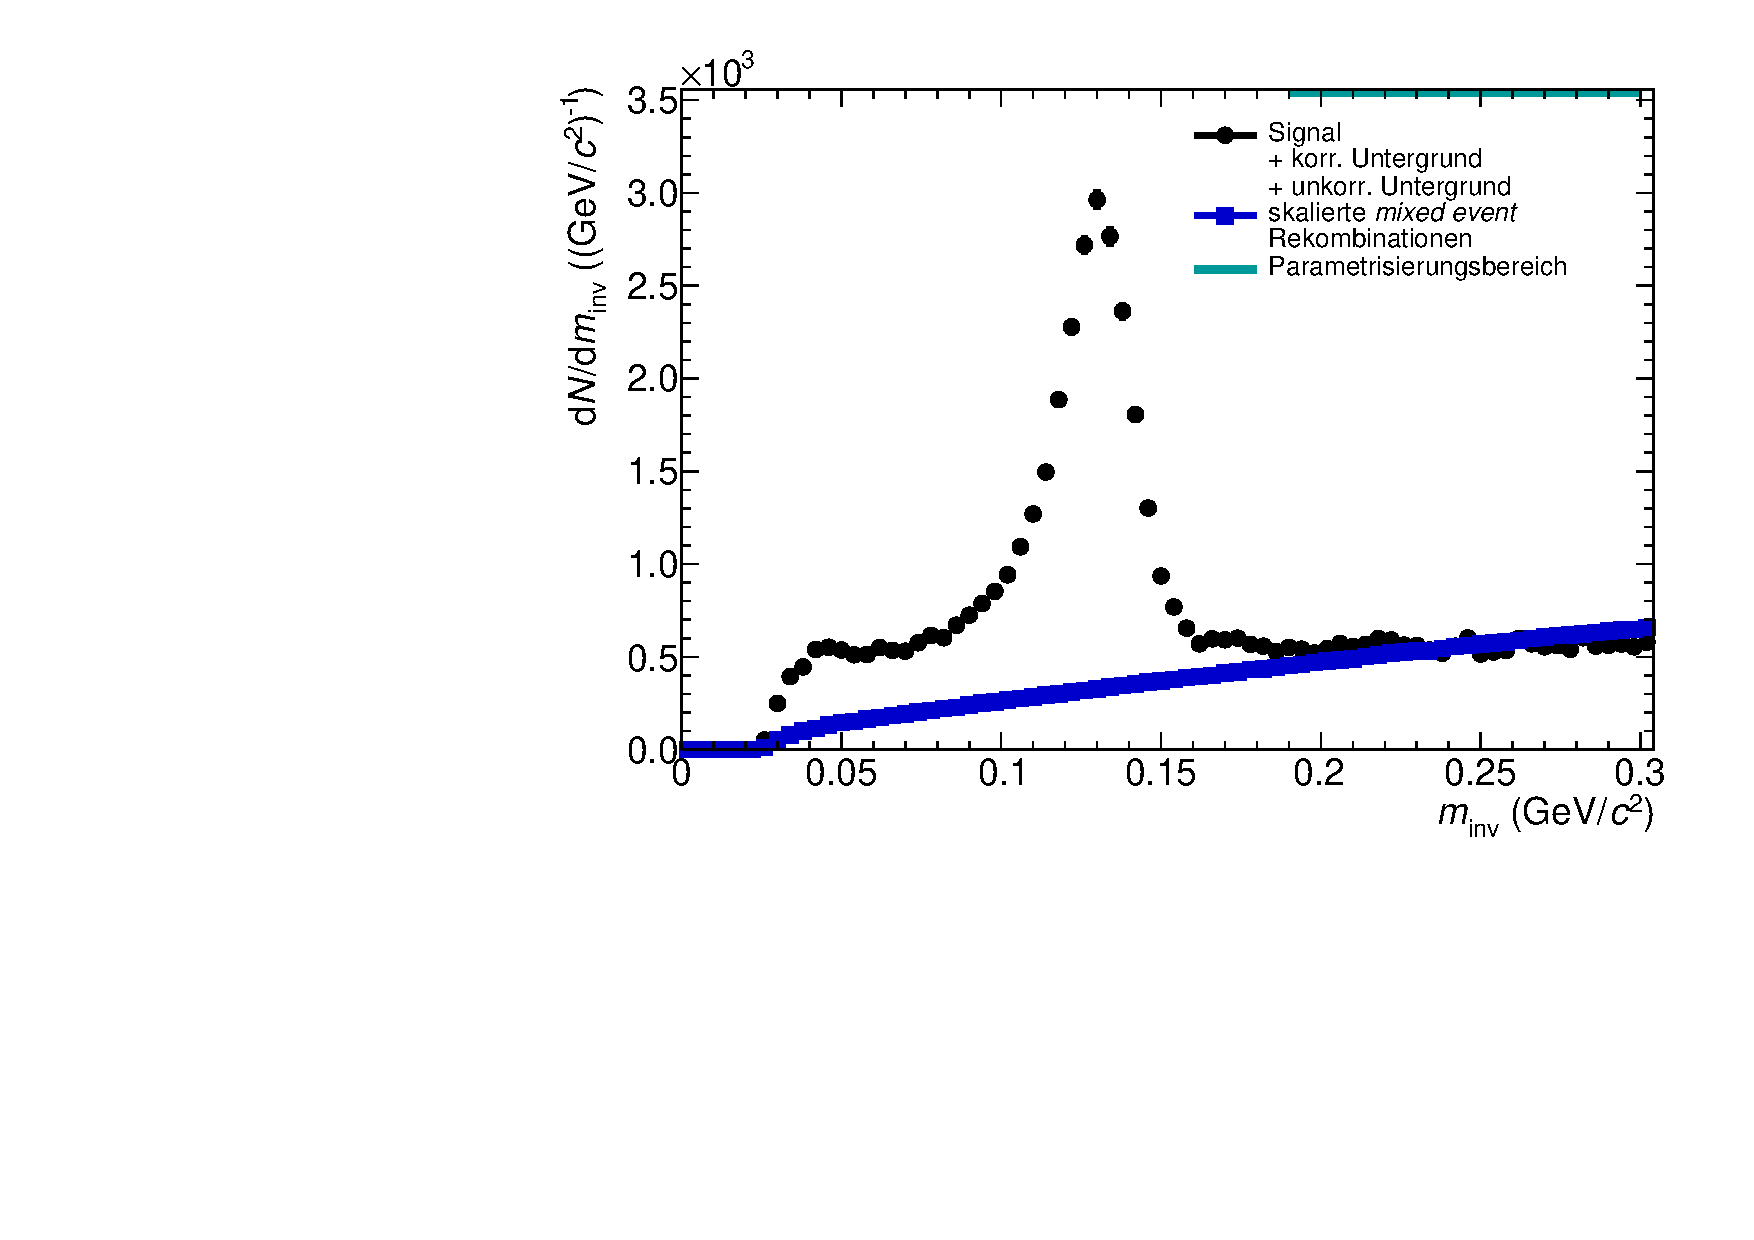
\includegraphics[width=.75\linewidth]{hUncorrBkgNorm.pdf}
\caption{Nach Gleichung \ref{eqBackSkalierung} skalierte {\it mixed event} Kombinationen als Abschätzung des unkorrelierten Untergrunds zusammen aufgetragen mit Signal zuzüglich beiden Untergrundkomponenten wie in Abbildung \ref{figSignalPlusBkg}.}
\label{figUncorrBkgNorm}
\end{figure}
\newline
Abbildung \ref{figUncorrBkgNorm} zeigt die skalierten \textit{mixed event} Kombinationen und das Signal zusammen mit dem korrelierten und dem unkorrelierten Untergrund.
Nachdem der unkorrelierte Untergrund abgeschätzt wird, wird dieser von der Verteilung der invarianten Masse aus der \textit{same event} Methode subtrahiert.
\begin{figure}[tp]
\centering
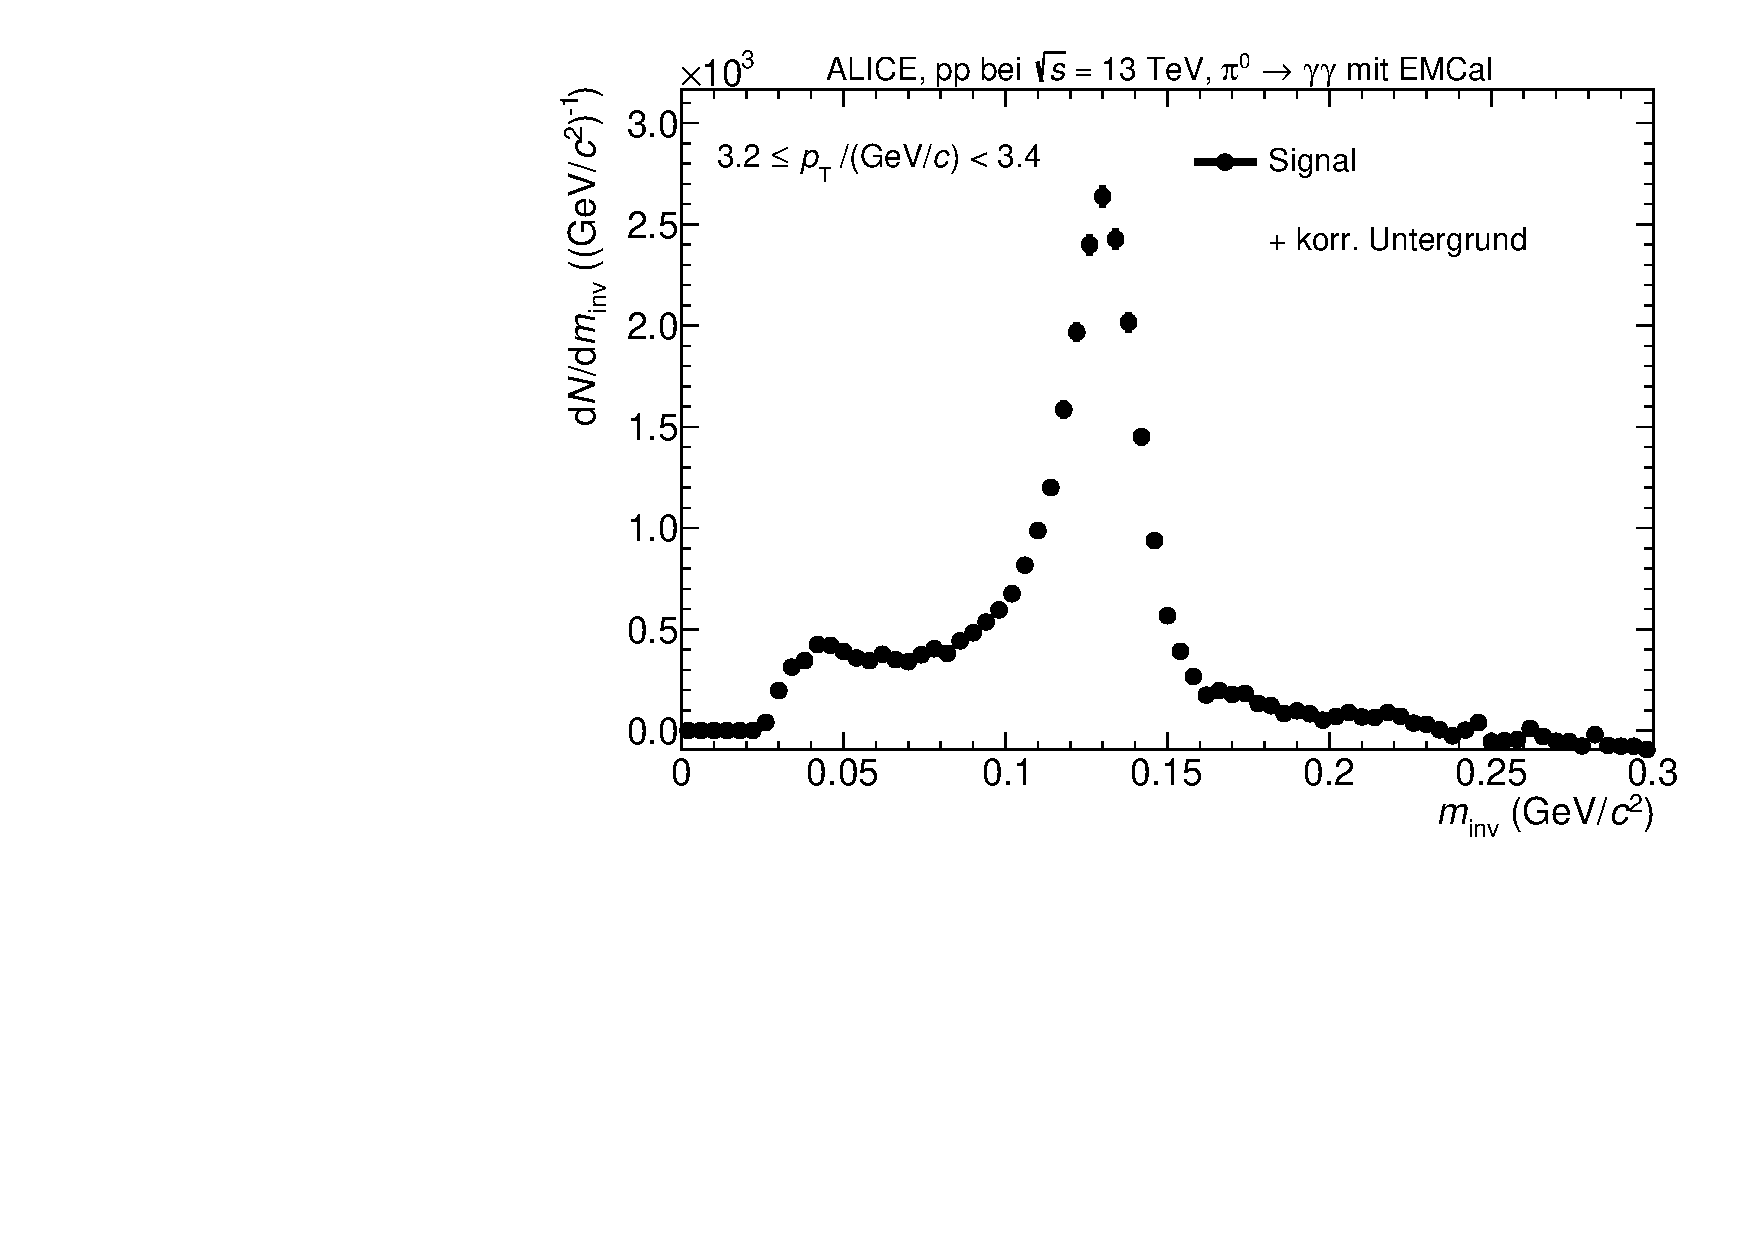
\includegraphics[width=.75\linewidth]{hInvMass_Data.pdf}
\caption{Signal nach Abzug des unkorrelierten Untergrunds.}
\label{figInvMass_Data}
\end{figure}
\newline
Abbildung \ref{figInvMass_Data} zeigt eine Verteilung der invarianten Masse aus der \textit{same event} Methode, nachdem die skalierten Kombinationen aus der \textit{mixed event} Methode, als Abschätzung der unkorrelierten Untergrunds, abgezogen wurden.
%Da Photonen durch Paarbildung in ein Elektron und ein Positron konvertieren können, bestehen einige Photonenkandidaten aus \textit{Clustern} aus nur einem der beiden Konversionsprodukte.
%Diese Photonenkandidaten weisen dann eine geringere Energie auf, als das eigentliche Photon besaß.
%Durch Kombinationen mit diesen Photonenkandidaten entstehen Einträge bei einer invarianten Masse, die meistens geringer ist als die Masse von $\pi^{0}$, obwohl beide Photonenkandidaten dem selben $\pi^{0}$ entstammen.
%Deshalb wird bei kleineren invarianten Massen links vom Peak ein Teil des Signals erwartet, jedoch auch korrelierter Untergrund.
\newline
Der nächste Schritt in der Analyse neutraler Pionen ist die Bestimmung des korrelierten Untergrunds.
Das Abschätzen mit einer linearen Funktion hat sich als gängigste Methode zur Abschätzung des korrelierten Untergrunds entwickelt und wird im Folgenden als Standardmethode bezeichnet.
In dieser Arbeit wird der korrelierte Untergrund sowie das reine $\pi^{0}$-Signal mit Hilfe von Monte Carlo Templates bestimmt.
Die Ergebnisse der Analyse mit Hilfe von Monte Carlo Templates, sowie mit der Standardmethode werden miteinander vergleichen, um eine Aussage über den möglichen Nutzen von Analysen mit Hilfe von Monte Carlo Templates treffen zu können.
Im folgenden Abschnitt wird zunächst die Standardmethode kurz erläutert.

\section{Absch{\"a}tzung des korrelierten Untergrunds mit der Standardmethode} \label{s3s4}
%Wie im Abschnitt zuvor erwähnt, wird in diesem Abschnitt die Extraktion des Signals, beziehungsweise die Abschätzung des korrelierten Untergrunds durch Parametrisieren von Funktionen kurz vorgestellt.
%\newline
Da es sich bei dem Signal um eine statistische Größe handelt, wird eine gaußförmig Funktion benutzt, um das Signal zu beschreiben.
%Der Mittelwert der Signalfunktion stellt einen freien Parameter dar und entspricht im Optimalfall der $\pi^{0}$-Masse.
%Als zwei weitere freie Parameter werden die Amplitude der Signalfunktion, sowie die Standardabweichung vom Mittelwert benutzt.
\newline
Wie bereits diskutiert, können Photonenkandidaten aus Konversionen eine geringere Energie tragen, als nicht konvertierte Photonenkandidaten.
Dadurch liegt die                                                                                                                                                                                                                                                                                                                                                                                                                                                                                                                                                                                                                                                                                                                                                                                                                                                                                                                                                                                                                                                                                                                                                                                                                                                                                                                                                                                                                                                                                                                                                                                                       e Masse in Kombinationen mit Photonenkandidaten aus Konversionen bei kleineren Werten, als die $\pi^{0}$ Masse, obwohl die Photonenkandidaten von dem gleichen $\pi^{0}$ stammen.
Deshalb wird die gaußförmig Funktion zur Beschreibung des Signals um eine sogenannte \textit{Tail} Komponente erweitert.
Die \textit{Tail} Komponente wird durch eine exponentielle Funktion beschrieben, die anschaulich als eine Abweichung der gaußförmig Funktion des Signals auf der linken Seite der $\pi^{0}$ Masse betrachtet werden kann.
\newline
Für den korrelierten Untergrund wird eine lineare Funktion, abhängig von der invarianten Masse, angenommen.
\newline
Die drei Funktionen werden zusammen durch Variation ihrer freien Parameter an die Verteilung angepasst.
Als freie Parameter für den korrelierten Untergrund wird der Schnittpunkt mit der y-Achse, sowie die Steigung der linearen Funktion verwendet.
\begin{figure}[tp]
\centering
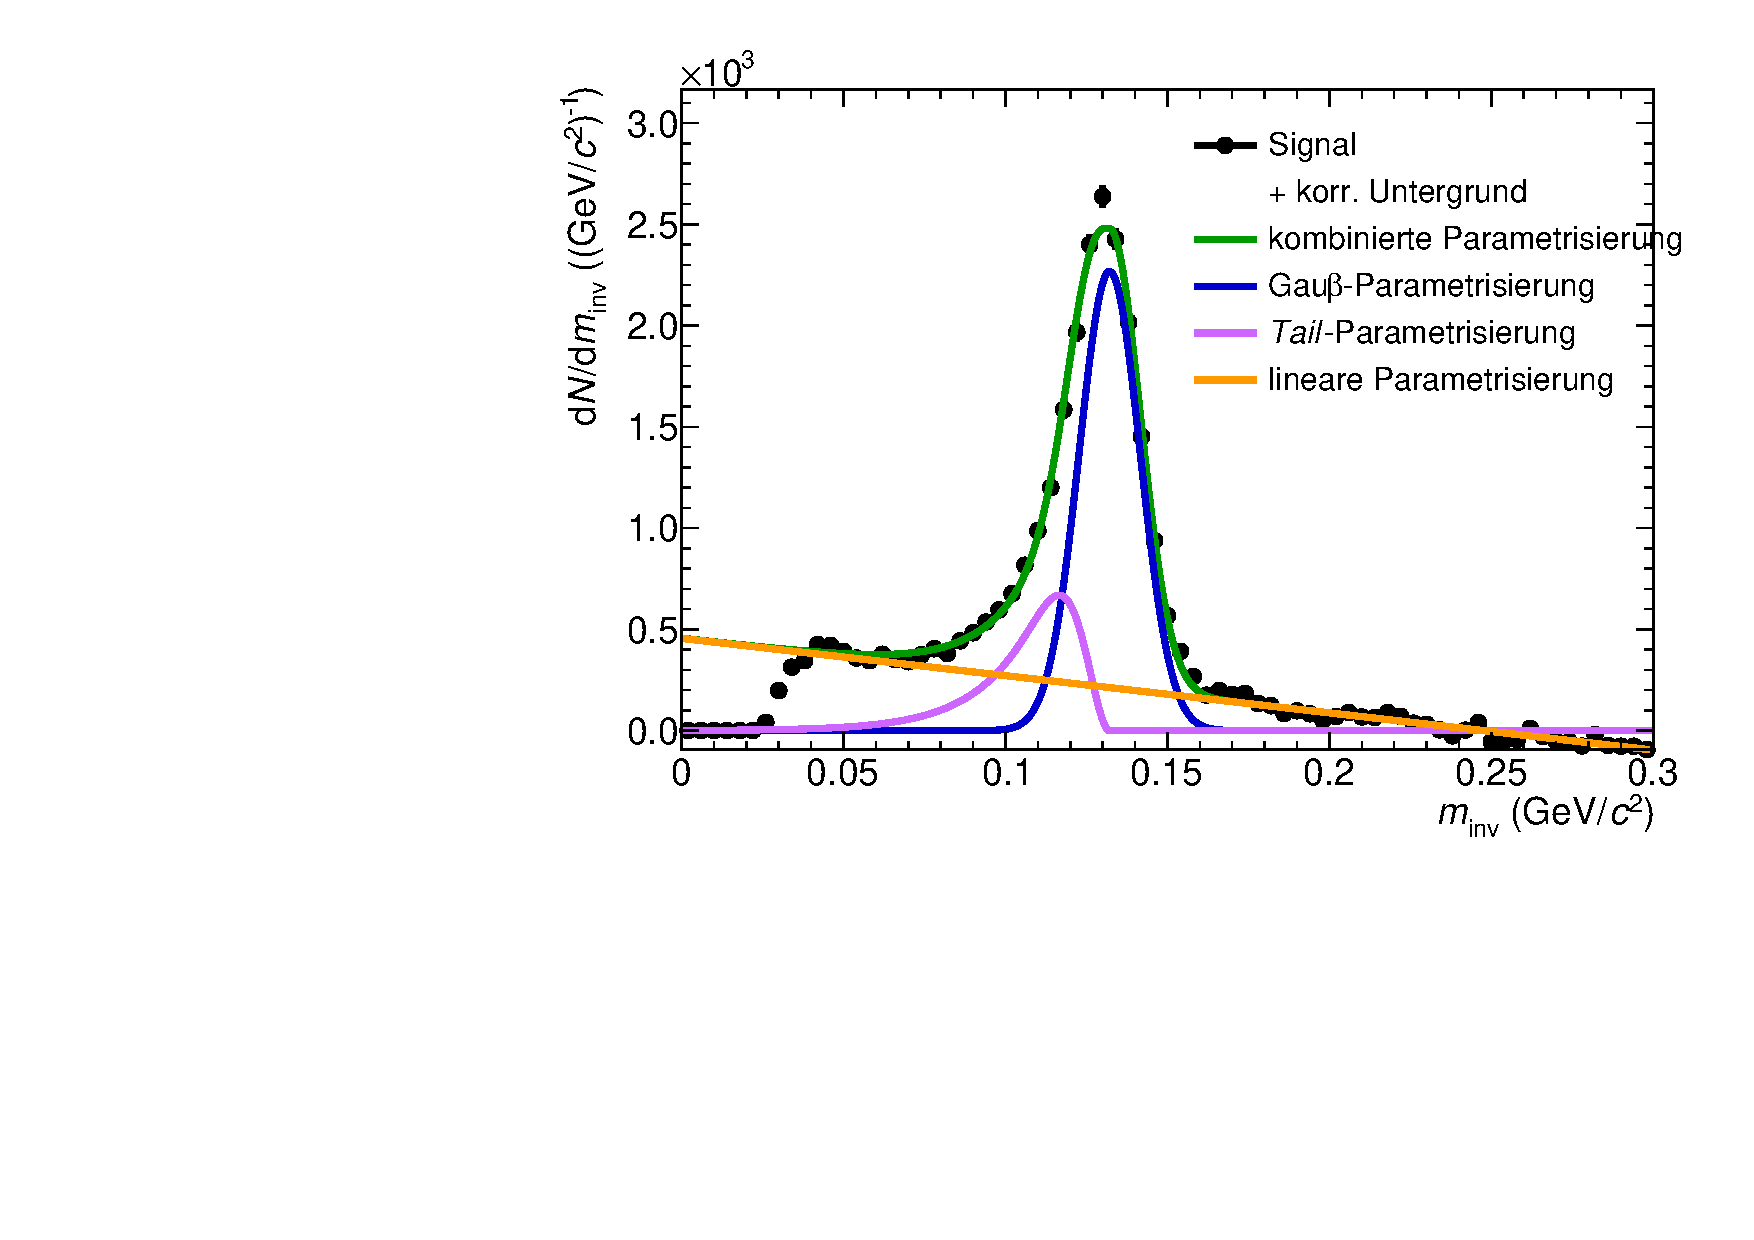
\includegraphics[width=.75\linewidth]{StandardParam.pdf}
\caption{Signal mit korreliertem Untergrund sowie den Funktionen zur Beschreibung des Signals mit korreliertem Untergrund.}
\label{figStandardParam}
\end{figure}
\newline
Abbildung \ref{figStandardParam} zeigt die Verteilung der invariante Masse bestehend aus Signal und korreliertem Untergrund, sowie das Ergebnis einer beschriebenen Anpassung.
Die grüne Kurve entspricht der Summe der drei einzelnen Komponenten, wobei die Gauß-Funktion in blau, die \textit{Tail}-Funktion in pink und die lineare Funktion in orange, dargestellt werden.
Dabei wird deutlich, dass durch die Abschätzung des korrelierten Untergrunds über die lineare Funktion bei einer invarianten Masse von etwa $0\,06\text{ GeV}/c^{2}$, kein beziehungsweise kaum Signal vorliegt.
Zu noch kleineren Massen hin schneidet die Anforderung an den Öffnungswinkel in den Verlauf, welcher nicht durch die Funktionen beschrieben wird.
\newline
Im folgenden Abschnitt wird die Abschätzung des korrelierten Untergrunds mit Hilfe von Templates beschrieben.

\section{Peakextraktion mit Hilfe von Parametrisierungen von Templates} \label{s3s5}
Um das Signal extrahieren zu können mit Hilfe von Templates wird, wie auch bei der Standardmethode, zunächst eine Abschätzung des korrelierten Untergrunds gemacht.
Hierfür werden zwei Templates an die Daten angepasst, vergleichbar wie in der Standardmethode eine Funktion bestehend aus drei Teilen an die Daten angepasst wurde.
Ein Template des Signals wird verwendet um das gesamte $\pi^{0}$ Signal zu beschreiben.
Im Vergleich zur Standardmethode entspricht das dem Gau{\ss}-Teil sowie dem \textit{Tail}-Tail der Funktion.
Der korrelierte Untergrund wird durch eine eigenes Template abgeschätzt, statt durch einen lineare Funktion.
\newline
Im folgenden Abschnitt wird das Template des Signals diskutiert. 

\subsection{Template des Signals} \label{s3s5s1}
Das Template des Signals wird mit Hilfe der Information der Monte Carlo Simulation erstellt.
Dabei wird ausgenutzt, dass in der Simulation bekannt ist, welchen Ursprung welches Teilchen hat und welches Teilchen auf das EMCal trifft.
Dadurch wird ermöglicht, genau bestimmen zu können, ob ein Teilchen aus dem Zerfall eines $\pi^{0}$ oder einem anderen Prozess stammt und ob es sich dabei um ein Photon, ein konvertiertes Elektron oder Positron, oder ein anderes Teilchen handelt.
\begin{figure}[tp]
\centering
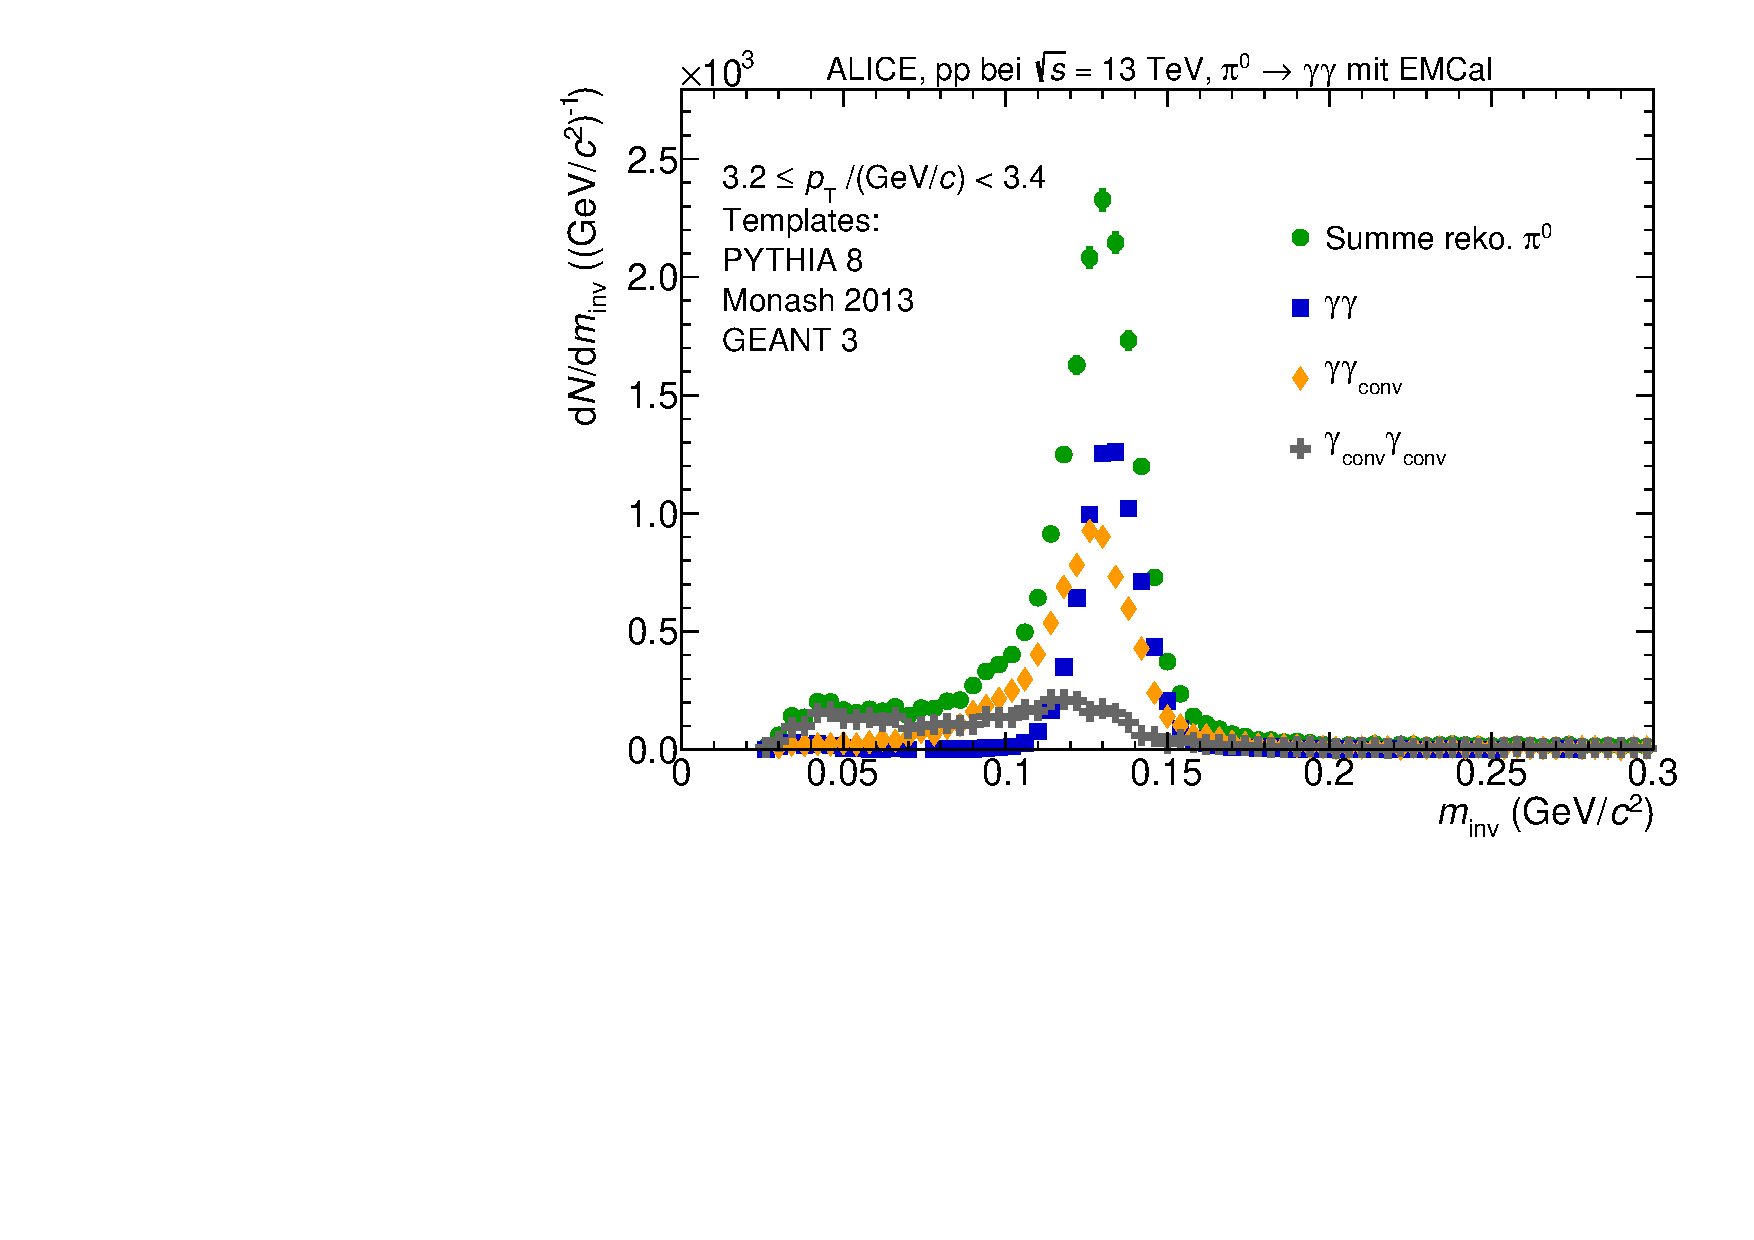
\includegraphics[width=.75\linewidth]{PeakTemplateMotivation10_Data_2016.pdf}
\caption{Template des Signals (grün) mit seinen drei Teilkomponenten.
Diese bestehen aus Kombinationen mit zwei Photonen (blau), einem Photon und einem Konversionselektron oder Konversionspositron (gelb) und zwei unterschiedlichen Konversionselektronen oder Konversionspositronen (grau).}
\label{fig:SigTemp}
\end{figure}
\newline
%Joshuas Problem mit dem Satz?
Abbildung \ref{fig:SigTemp} zeigt das Template des Signals in grün, sowie die Aufteilung des Signals in seine einzelnen Komponenten.
%wording anders?
Die Komponenten setzen sich aus den drei möglichen Kombinationen von \textit{Clustern} zusammen.
Zum einen aus \textit{Clustern} aus Photonen, in der Abbildung als $\gamma$ bezeichnet, und zum anderen aus \textit{Clustern} aus einem Elektron oder Positron, die durch die Konversion  eines Photonen entstanden sind.
Letztere werden in der Abbildung durch $\gamma_\text{conv}$ symbolisiert.
\newline
In blau sind die Kombinationen aus zwei Photonen ($\gamma\gamma$) dargestellt, in gelb die Kombination aus Photon und Elektron oder Positron ($\gamma\gamma_\text{conv}$) und in grau die Kombination aus Konversionselektron oder Konversionspositron miteinander ($\gamma_\text{conv}\gamma_\text{conv}$).
\newline
Die Abbildung zeigt außerdem, wie zuvor angesprochen, dass bis $m_\text{inv}>0\,05 \text{ GeV}/c^{2}$ Signal vorliegt.
Der Anteil des Signals um diese invariante Masse besteht hauptsächlich aus zwei Teilchen aus einer Photonkonversion.
Genau dieser Teil des Signals wird nicht durch die Standardmethode berücksichtigt.
Durch das Berücksichtigen in der Analyse mit Hilfe der Templates kann ein größerer Anteil des Signals gezählt werden.
Deshalb wird eine geringere statistische Unsicherheit erwartet.

\subsection{Template des korrelierten Untergrunds} \label{s3s5s2}
Für die Bestimmung des Templates des korrelierten Untergrunds wird das Template des Signals von der Verteilung der invarianten Masse aus der Monte Carlo Simulation abgezogen, die im gleichen $p_\text{T}$-Intervall liegt wie das Template des Signals.
\begin{figure}[tp]
\centering
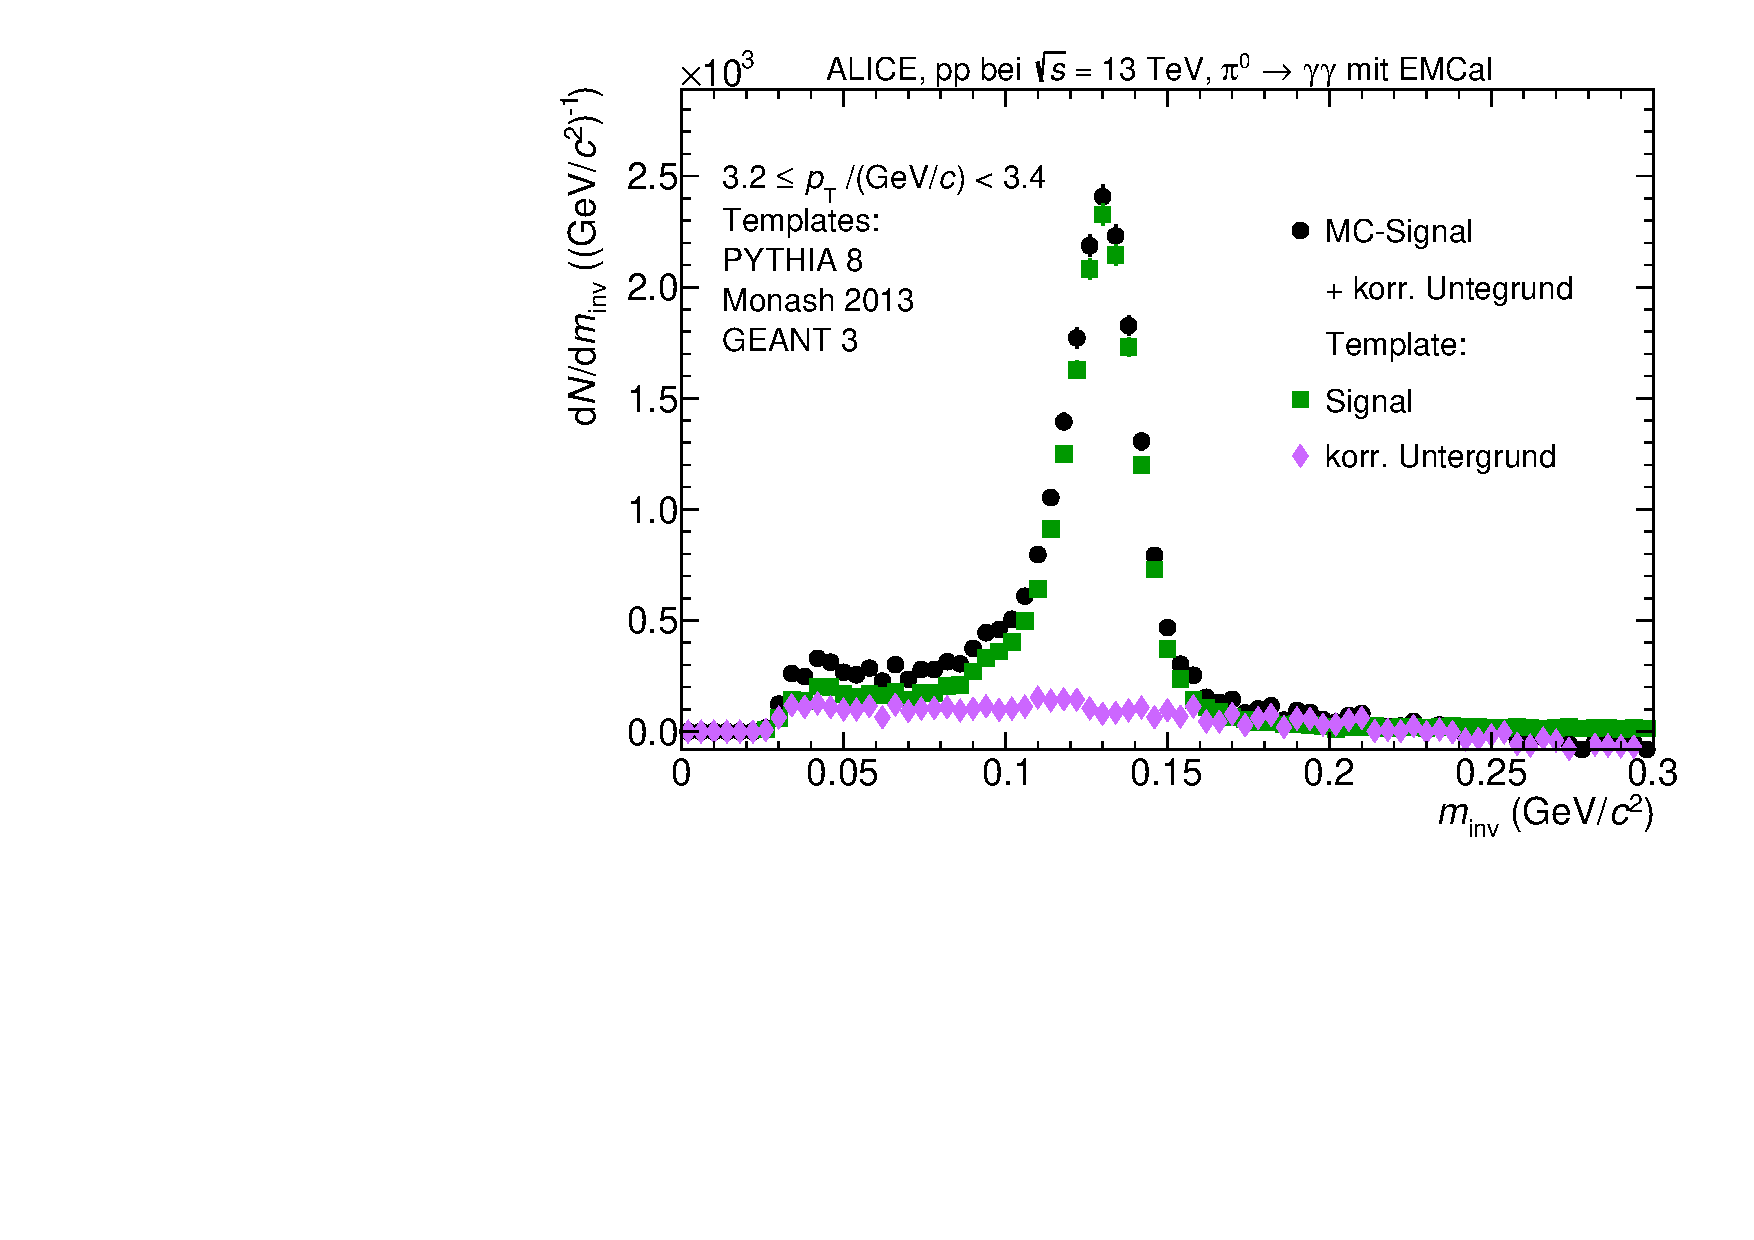
\includegraphics[width=.75\linewidth]{EntstehungUntergrund10_Data_2016.pdf}
\caption{Template des korrelierten Untergrunds in pink entstanden durch den Abzug des Templates des Signals (grün) von der Verteilung der invarianten Masse aus einer Monte Carlo Simulation (schwarz).}
\label{fig:BkgTemp}
\end{figure}
\newline
Abbildung \ref{fig:BkgTemp} zeigt die Anzahl \textit{Clusterpaare}, die aus dem Zerfall eines einzelnen $\pi^{0}$ stammen, als Funktion von $m_\text{inv}$ in schwarz.
In pink wird das Template des korrelierten Untergrunds dargestellt und in grün das Template des Signals.
Alle drei Verteilungen stammen aus dem $p_\text{T}$-Intervall $(3\,2 - 3\,4) (\text{GeV/}c)$.
Hierbei wird deutlich, dass in der Monte Carlo Simulation der korrelierte Untergrund im Bereich von $m_\text{inv} = 0,05 \text{ GeV/}c^{2}$ in der Größenordnung des Signals liegt.
In der Standardmethode wurde zuvor gezeigt, dass in diesem $m_\text{inv}$-Bereich der korrelierte Untergrund dominiert.
\newline
Für die Anpassung der Templates an die Daten wird, relativ zu den Werten der Einträge in den Templates, eine geringe statistische Unsicherheit der beiden Templates benötigt.
Um die Unsicherheit zu verkleinern, wird in dieser Arbeit der korrelierte Untergrund aus einem größeren $p_\text{T}$-Intervallen verwendet als die in dieser Analyse gewählten $p_\text{T}$-Intervalle.
Dieses Template wird im folgenden als kombiniertes Template des korrelierten Untergrunds bezeichnet, da das vergrößerte $p_\text{T}$-Intervall mehrere zuvor gewählten $p_\text{T}$-Intervalle kombiniert.
Dabei wird angenommen, dass sich nicht die Form, sondern nur die Anzahl der Einträge in den $p_\text{T}$-Intervallen unterscheidet.  
Für das kombinierte Template des korrelierten Untergrunds wird $p_\text{T} \geq 1\,8\text{ GeV}/c$ bis $p_\text{T} < 3\,2\text{ GeV}/c$ benutzt, da in diesem Bereich die statistische Unsicherheit am geringsten ist.
Um diese Methode zur Bestimmung des Template des korrelierten Untergrunds anwenden zu können, wird die Annahme getroffen, dass sich die Form des Template des korrelierten Untergrunds nicht ändert.
Lediglich die Anzahl der Einträge in den Templates des korrelierten Untergrunds variiert.
\begin{figure}[t!]
\centering
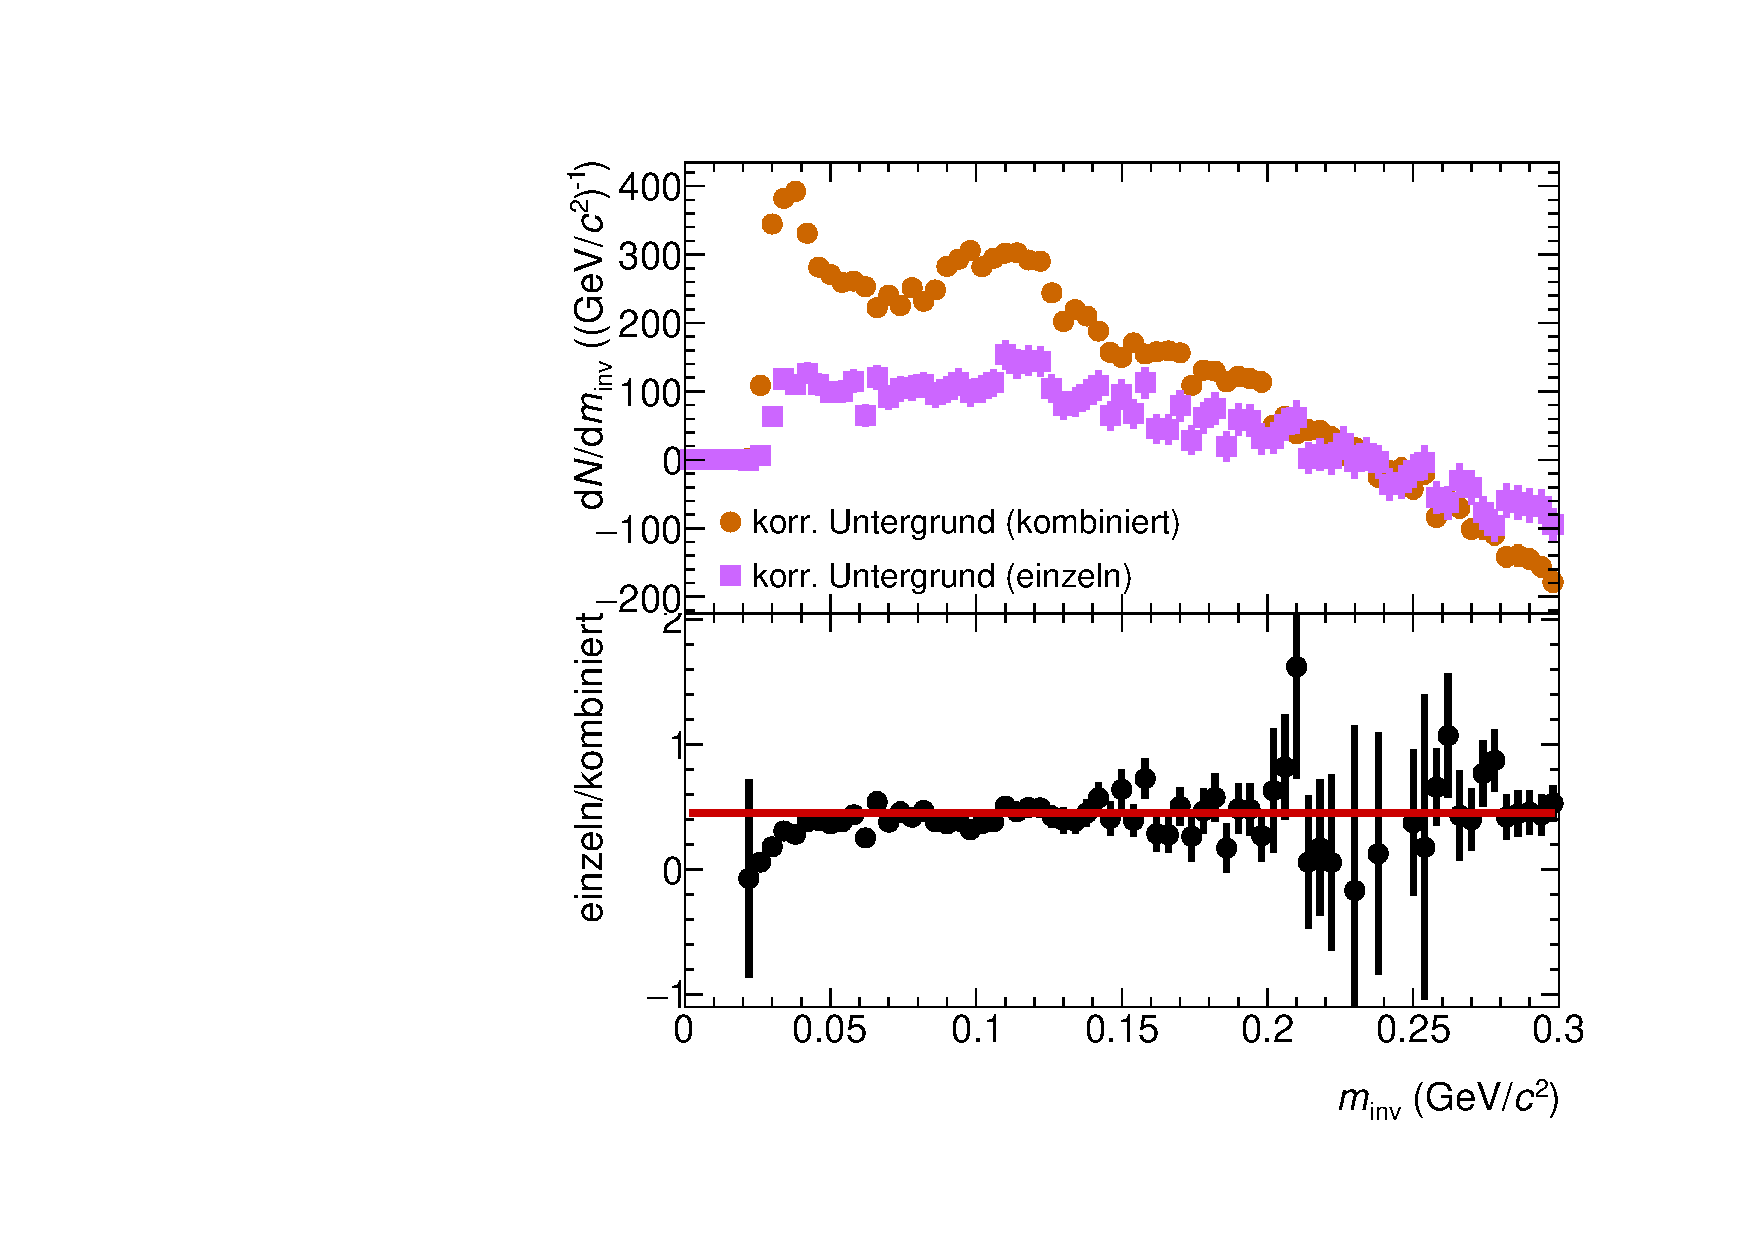
\includegraphics[width=.7\linewidth]{BackgroundWithRatio10_Data_2016.pdf}
\caption{\textbf{Oben:} Template des korrelierten Untergrunds aus einem einzelnen $p_\text{T}$-Intervall in pink und aus mehreren $p_\text{T}$-Intervallen kombiniert in orange.
\textbf{Unten:} Verhältnis der beiden Verteilungen in schwarz, sowie Parametrisierung einer Konstante an das Verhältnis in rot.}
\label{fig:BkgTempRatio}
\end{figure}
\newline
Abbildung \ref{fig:BkgTempRatio} (oben) zeigt in orange das kombiniertes Template des korrelierten Untergrunds und in pink das Template des korrelierten Untergrunds für das $p_\text{T}$-Intervall $(3\,2 - 3\,4) (\text{GeV/}c)$.
Die Abbildungen für die anderen $p_\text{T}$-Intervalle befinden sich in Anhang \ref{Appendix:A1}.
Um zu zeigen, dass die Annahme ihre Richtigkeit hat wird in Abbildung \ref{fig:BkgTempRatio} (unten) das Verhältnis aus einzelnen Templates des korrelierten Untergrunds zu dem Kombinierten dargestellt.
Die grüne Linie im unteren Teil der Abbildung basiert auf einer konstanten Parametrisierung des Verhältnisses.
Die getroffene Annahme wird bestätigt, da die konstante Parametrisierung und das Verhältnis gut miteinander übereinstimmen.
Die große Unsicherheit im Verhältnis um $m_\text{inv} = 0,225\text{ GeV}/c^{2}$ entsteht, da beide Templates an dieser Stelle eine Anzahl an Einträgen im Bereich nahe um die Null besitzen.
Teilt man zwei kleine Zahlen durch einander, so ändert sich der Quotientenwert stark, wenn man nur eine der beiden kleinen Zahlen leicht ändert.
Die Unsicherheit der Einträge der Templates repräsentieren eine mögliche Variation der Einträge.
Diese Unsicherheit im Falle des einzelnen Templates des korrelierten Untergrunds besitzt einen großen absoluten Wert verglichen mit den Werten der Einträge um $m_\text{inv} = 0,225\text{ GeV}/c^{2}$.
Dadurch wird auch die Unsicherheit auf den Quotientenwert deutlich größer, als in den anderen $m_\text{inv}$ Bereichen.
\newline
In Abschnitt \ref{s3s2} wurde bereits angesprochen, dass die Anforderung an den Öffnungswinkel von $p_\text{T}$ abhängt.
Um das kombinierte Template des korrelieren Untergrunds daran anzupassen wird eine für diesen Zweck angepasste Monte Carlo Simulation betrachtet.
In der Simulation werden $\pi^{0}$ mit zufälliger Energie simuliert, die in zwei Photonen zerfallen.
Die Photonen müssen dann auf einen Raumwinkel auftreten um als detektiert zu gelten, der der Abdeckung des EMCals entspricht.
Die Photonen werden hierbei nicht durch \textit{Cluster} repräsentiert.
Dadurch wird verhindert, dass mehrere Teilchen zu einem \textit{Cluster} zusammengefasst werden können.
Die Photonen werden paarweise kombiniert, wie bei der \textit{Clusterkombination}.
Dabei wird einmal die Anforderung an den Öffnungswinkel gestellt wie sie in der Analyse vorliegt und einmal wird keine Anforderung an den Öffnungswinkel gestellt.
In beiden Fällen werden so viele $\pi^{0}$ erzeugt, dass am Ende die gleiche Anzahl an Photonenpaaren kombiniert wurde.
Daraus entstehen zwei Verteilungen, die die Anzahl kombinierter Photonenpaare als Funktion von $m_\text{inv}$ und $p_\text{T}$ darstellen, einmal für den Fall, dass es keine Anforderung an den Öffnungswinkel gibt und einmal mit der Anforderung an den Öffnungswinkel.
Da beide Teilsimulationen die gleiche Anzahl an kombinierten Photonenpaaren haben, kann aus dem Verhältnis der Verteilung mit Anforderung an den Öffnungswinkel zur Verteilung ohne Anforderung an den Öffnungswinkel, bestimmt werden, wie wahrscheinlich es ist einen Photonenkombination bei einem bestimmen $m_\text{inv}$ und $p_\text{T}$ zu messen.
Mit Hilfe dieser Wahrscheinlichkeitsverteilung werden die Templates des korrelierten Untergrunds, die das kombinierte Template des korrelierten Untergrunds bilden, an die unterschiedlichen $p_\text{T}$-Intervalle skaliert.
Dadurch konnten größere Abweichungen für kleinere invariante Massen vermieden werden.
\newline
In Abschnitt \ref{s4s2} wird für die Bestimmung der systematischen Unsicherheit die Wahl des Templates des korrelierten Untergrunds variiert.
\newline
Zum einen werden die Templates des korrelierten Untergrunds aus dem jeweiligen $p_\text{T}$-Intervall verwendet, aus dem auch die Verteilung der invarianten Masse und das Template des Signals kommen.
Wie bereits erwähnt wird die statistische Unsicherheit, relativ gesehen zu den Werten der Templates, groß.
Tabelle \ref{tab:IntAndError} im Anhang \ref{Appendix:A2} zeigt die Integrale sowie die Unsicherheit der verschiedenen $p_\text{T}$-Intervalle.
Die statistischen Unsicherheiten sind für $6,0 \leq p_\text{T}/\text{ GeV}/c < 8,0 $ groß genug, sodass die Werte des Template des korrelierten Untergrunds mit Null kompatibel sind.
Das hat zur Folge, dass je stärker das Template des korrelierten Untergrunds skaliert wird, desto größer werden die statistischen Unsicherheiten.
Effektiv wird nur die statistische Unsicherheit erhöht, was $\chi^{2}$ verkleinert.
Dadurch wird die Anpassung über $\chi^{2}$-Minimierung verfälscht.
Die Berechnung von $\chi^{2}$ wird im nächsten Abschnitt genauer erläutert.
\newline
Für $p_\text{T} > 8,0 \text{ GeV}/c$ liegen die Integrale im negativen Bereich, auch innerhalb der statistischen Unsicherheit.
Da ein negativer korrelierter Untergrund physikalisch nicht sinnvoll ist, werden die Templates des korrelierten Untergrunds in diesem $p_\text{T}$-Bereich mit Null skaliert.
\newline
Zum anderen wird die Kombination variiert, sodass das Template des korrelierten Untergrunds nicht aus einem festen vergrößerten $p_\text{T}$-Intervall stammt.
Stattdessen wird das $p_\text{T}$-Intervall eines einzelnen Templates des korrelierten Untergrunds ausgeweitet, bis das Intervall mindestens $4\text{ GeV}/c$ umfasst.
Da also die nächsten Nachbarintervalle zusammengefasst werden, wird diese Methode zur Bestimmung der Template des korrelierten Untergrunds als nächste Nachbarn Methode bezeichnet.
Im Gegensatz zur Methode mit dem kombinierten Template wird in dieser Methode eine etwaige Änderung der Form des korrelierten Untergrunds berücksichtigt.
Die Änderung des korrelierten Untergrunds darf dabei allerdings nur kontinuierlich in $p_\text{T}$ stattfinden.
Durch das verbreitern aller $p_\text{T}$-Intervalle überlappen sich die $p_\text{T}$-Bereiche aus denen die unterschiedlichen Templates des korrelierten Untergrunds stammen.
Die dadurch entstehende Korrelation in den statistischen Unsicherheiten der verschiedenen kombinierten Templates des korrelierten Untergrunds kann dabei nur grob abgeschätzt werden. 
\newpage
\noindent
Aus den genannten negativ Gründen, sowie der Bestätigung der Annahme, dass die Form des korrelierten Untergrund nicht von $p_\text{T}$ abhängt, werden beide Methoden für die Bestimmung der systematischen Unsicherheiten benutzt und nicht als Standard in dieser Analyse.
\newline
Im Folgenden Abschnitt werden die Templates des Signals und des korrelierten Untergrunds so parametrisiert, dass sie die Daten nach Abschätzung des unkorrelierten Untergrunds bestmöglich beschreiben.

\subsection{Parametriesierungsmethode} \label{s3s5s3}
Die Parametrisierung der Templates des Signals und des korrelierten Untergrunds erfolgt durch die sogenannte $\chi^{2}$-Minimierung.
$\chi^{2}$ gibt dabei ein Maß an, wie gut eine Verteilung an gegebene Daten passt.
Je kleiner $\chi^{2}$ ist, umso besser beschreibt die Verteilung die Daten.
Als freie Parameter werden zwei Skalierungsfaktoren benutzt, einmal ein Skalierungsfaktor für das Template des Signals (SF\textsubscript{Signal}) und einmal ein Skalierungsfaktor für das Template des korrelierten Untergrunds (SF\textsubscript{korr. Untergrund}).
Für $\chi^{2}$ gilt dann:
\begin{align}
\chi^{2} = \sum_{i}\left(\frac{\text{SF}_\text{Signal}\cdot x_{i}+\text{SF}_\text{korr. Untergrund}\cdot y_{i}-z_{i}}{\sqrt{\left(\text{SF}_\text{Signal}\cdot\Delta x_{i}\right)^{2}+\left(\text{SF}_\text{korr. Untergrund}\cdot\Delta y_{i}\right)^{2}+\left(\Delta z\right)^{2}}}\right)^{2}
\label{eq:Chi2}
\end{align}
Hierbei steht $x$ für das Template des Signals, $y$ für das Template des korrelierten Untergrunds und $z$ für die Verteilung der invarianten Masse nach Abzug der unkorrelierten Untergrunds.
Letzteres stammt dabei wieder aus den gemessenen Daten und nicht wie im Abschnitt davor aus einer Simulation.
Der Index $i$, über den summiert wird, läuft über die Intervalle in der invarianten Masse innerhalb des Parametrisierungsbereiches.
Der Parametrisierungsbereich wird so gewählt, dass die untere Seite außerhalb des Bereiches liegt wo die Anforderung an den Öffnungswinkel Kombinationsmöglichkeiten ausschließt.
Um diese Werte zu bestimmen wird das Ergebnis der vereinfachten Monte Carlo Simulation benutzt.
\begin{figure}[tp]
\centering
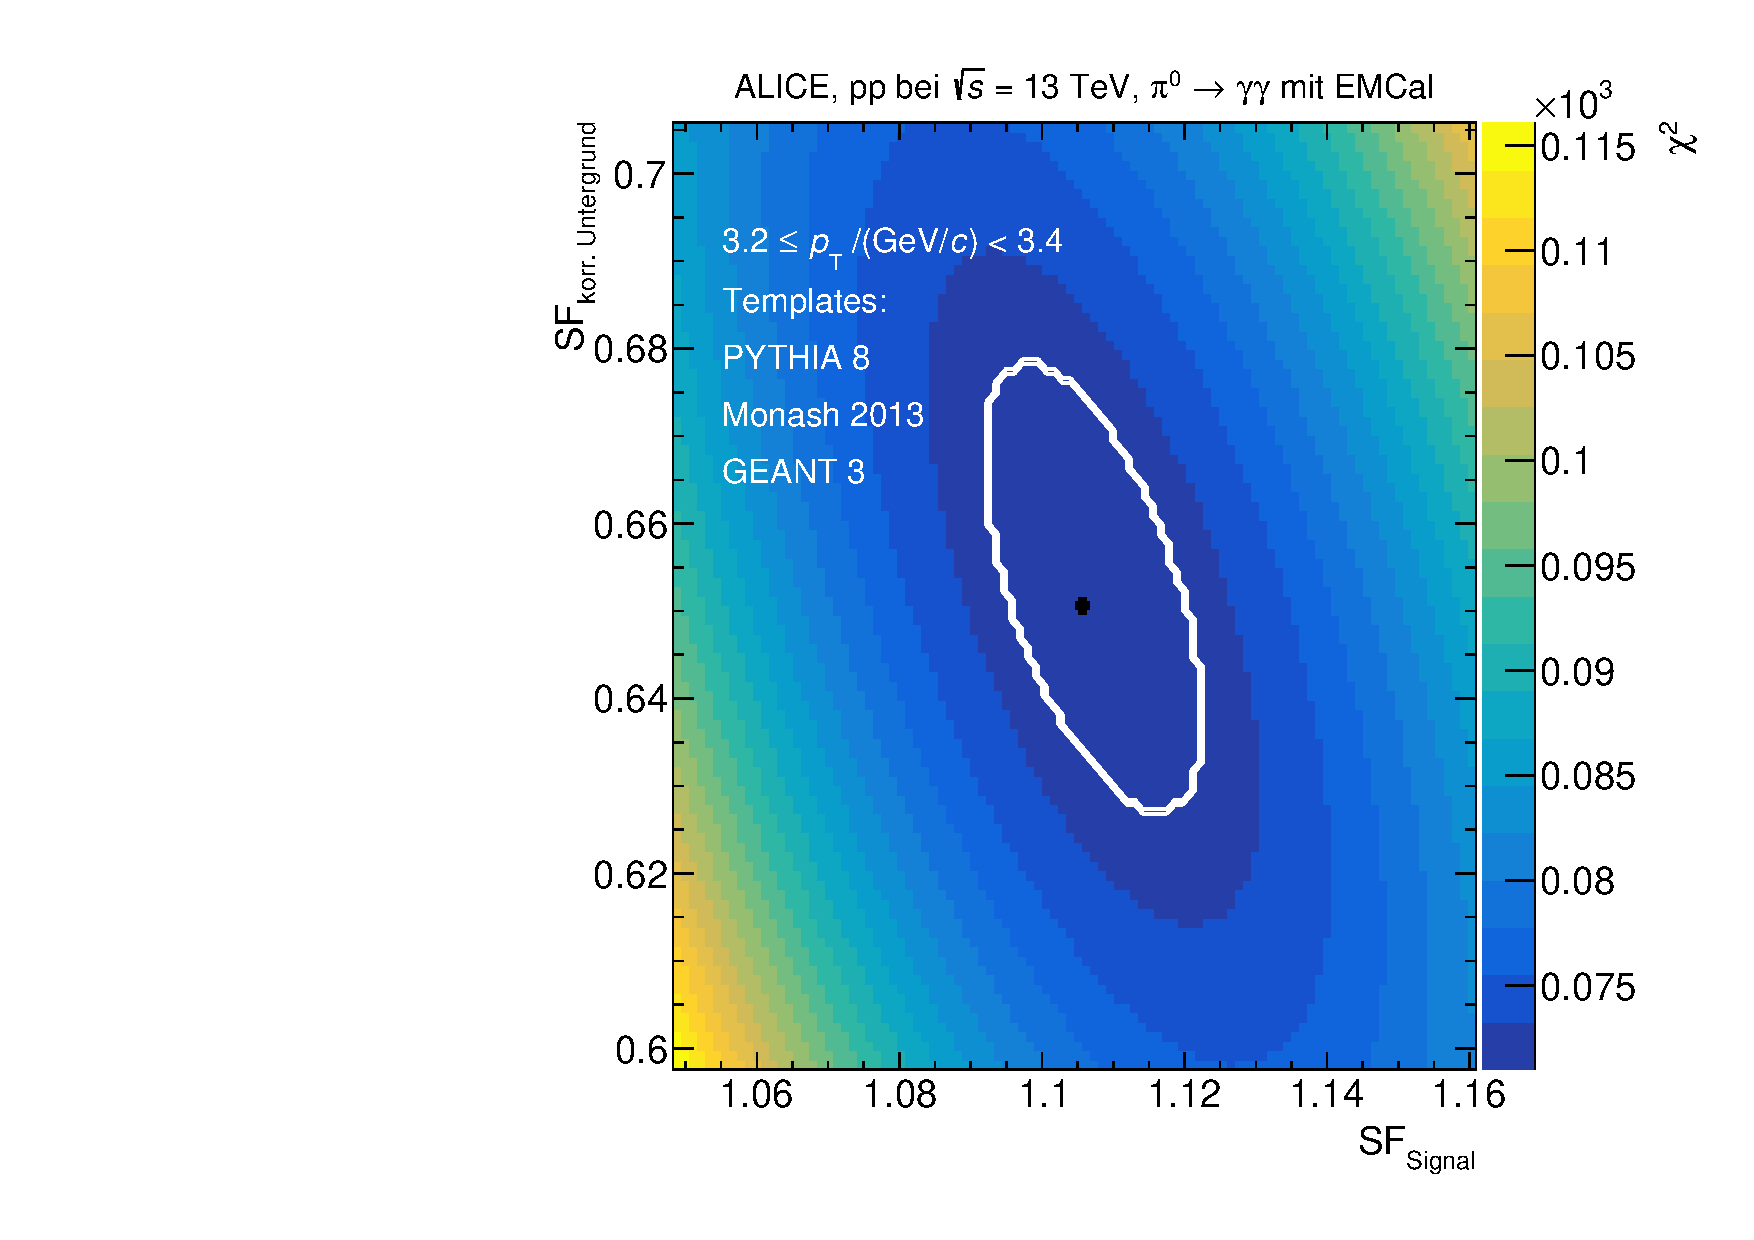
\includegraphics[width=.65\linewidth]{Chi2Map10_Data_2016.pdf}
\caption{$\chi^{2}$ in Abhängigkeit der Skalierungsfaktoren für das Template des Signals und das Template des korrelierten Untergrunds in einem $p_{\text{T}}$-Intervall von $(3\,2 - 3\,4)(\text{GeV}/c)$.
Die weiße Kurve makiert die Unsicherheit auf $\chi^{2}_\text{min}$.}
\label{fig:Chi2Map}
\end{figure}
\newline
Abbildung \ref{fig:Chi2Map} zeigt die Verteilung von $\chi^{2}$ für unterschiedliche Kombinationen der beiden Skalierungsfaktoren im $p_{\text{T}}$-Intervall $(3\,2 - 3\,4)(\text{GeV}/c)$.
$\chi^{2}_\text{min}$ liegt bei dem schwarzen Punkt in der Mitte des Bildes.
Die weiße Kurve, die das Minimum umgibt, gibt die Unsicherheit bezüglich der beiden Skalierungsfaktoren an.
Die Werte auf der weißen Kurve liegen werden berechnet durch $\left(\chi^{2}_\text{min}+1\right)$ \cite{book:chi2}.
\newline
Um die Stabilität der Methode zu prüfen wird $\frac{\chi^{2}_\text{min}}{ndf}$ in Abhängigkeit von $p_{\text{T}}$ betrachtet.
Der Nenner ndf steht für die Anzahl der Freiheitsgrade (in englisch \textit{\textbf{n}umbers of \textbf{d}egrees of \textbf{f}reedom}).
Die Anzahl an Freiheitsgraden setzt sich dabei aus zwei Teilen zusammen.
Zum einen gilt jeder Datenpunkt in der Verteilung der invarianten Masse, der weder in Daten, noch in einem der Templates den Wert 0 besitzt und sich innerhalb des Parametrisierungsbereiches befindet, als ein Freiheitsgrad.
Zum anderen wird für jeden freien Parameter die Anzahl an Freiheitsgraden um eins reduziert.
Die Anforderungen an den Öffnungswinkel reduzieren zu höherem $p_{\text{T}}$ hin die Anzahl an Freiheitsgraden zunehmend, weshalb die Normierung von $\chi^{2}_\text{min}$ auf die Anzahl an Freiheitsgraden für einen $p_{\text{T}}$-differenzierten Vergleich notwendig ist.
Außerdem gibt der Wert von $\frac{\chi^{2}_\text{min}}{ndf}$ einen allgemeinen Hinweis auf die Güte der Parametrisierung.
Für $\frac{\chi^{2}_\text{min}}{ndf} > 1$ gilt, dass die Parametrisierung der Templates und die Verteilung der Daten immer weniger gut übereinstimmen.
Umgekehrt gilt für $\frac{\chi^{2}_\text{min}}{ndf} < 1$, dass die Unsicherheiten in der Verteilung der Daten oder den Templates zu groß sind, für eine sinnvolle Parametrisierung.
\begin{figure}[tp]
\centering
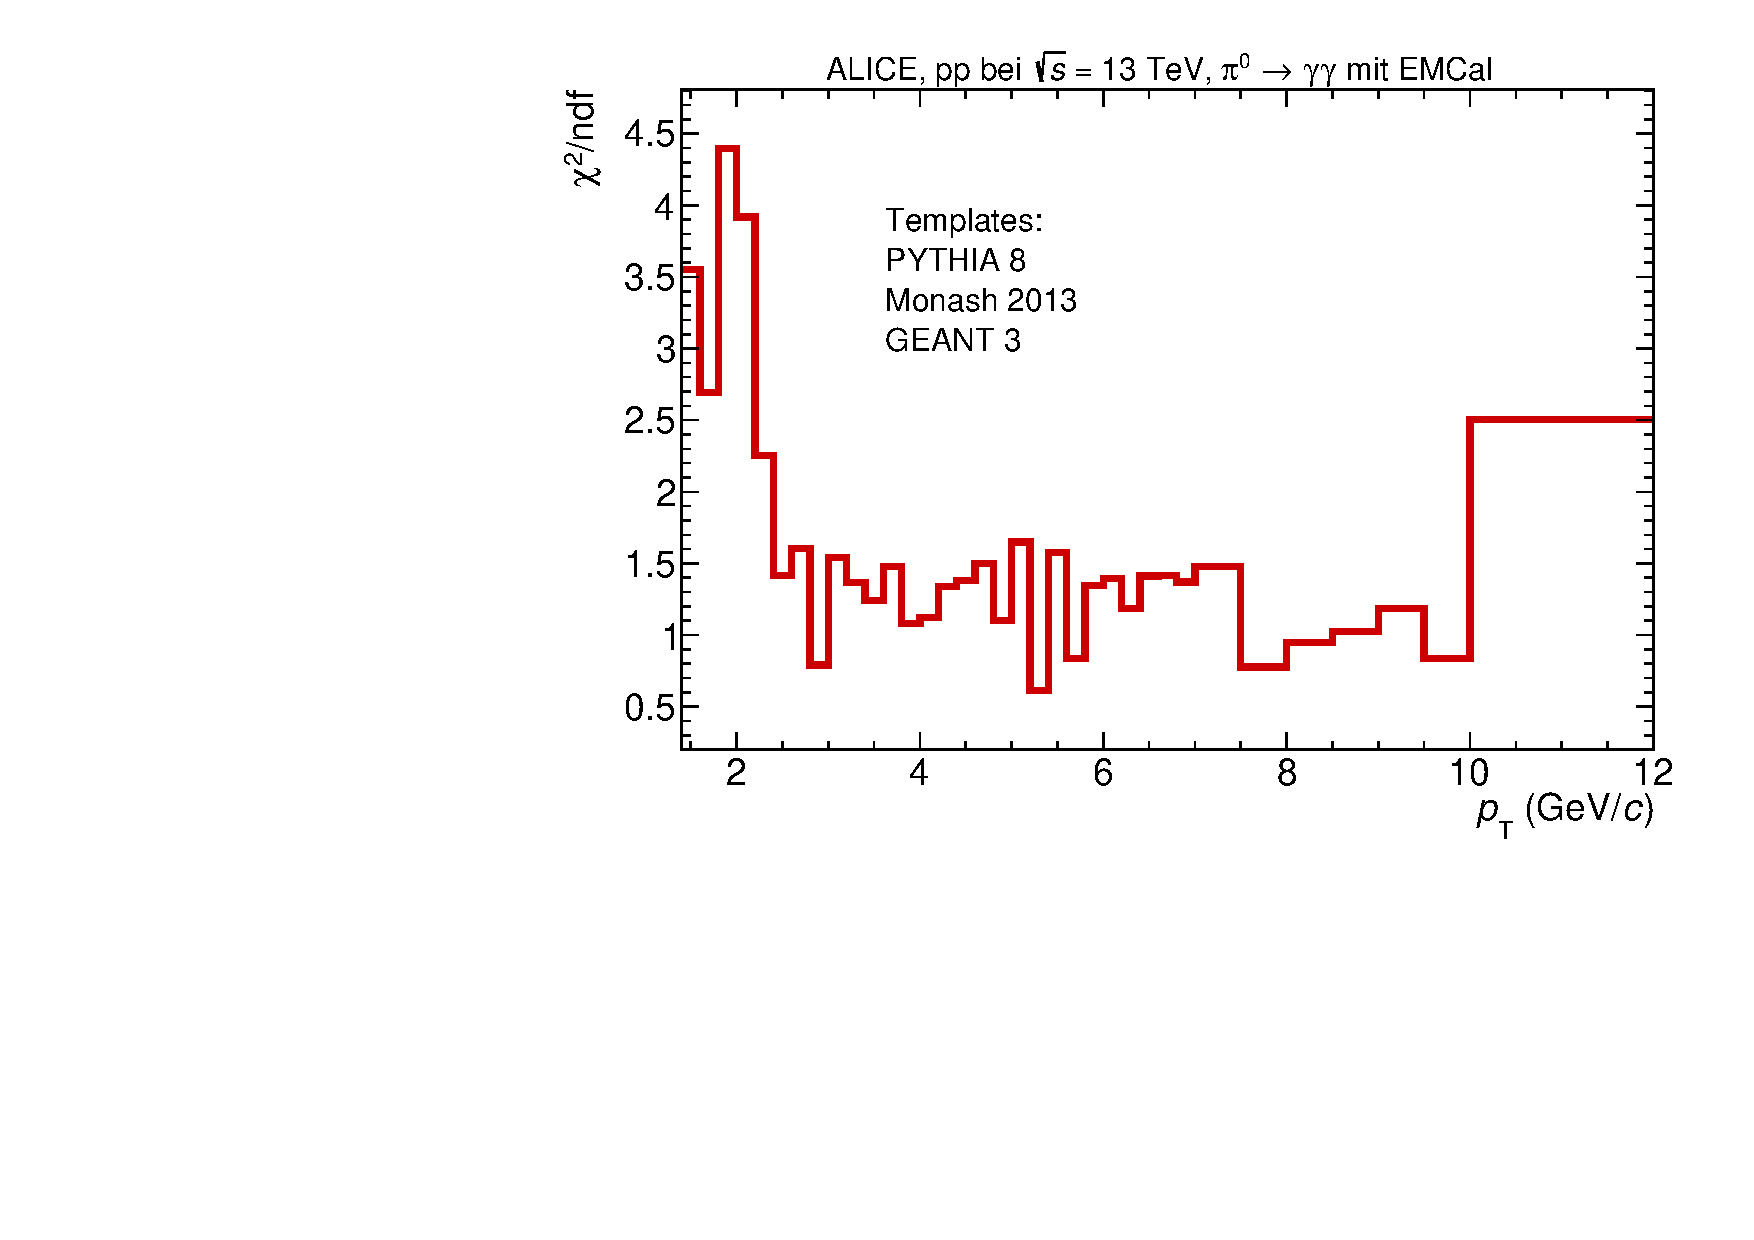
\includegraphics[width=.65\linewidth]{Chi2NoComp_Data_2016.pdf}
\caption{$\frac{\chi^{2}_\text{min}}{ndf}$ in Abhängigkeit von $p_{\text{T}}$.
}
\label{fig:Chi2pT}
\end{figure}
\newline
Abbildung \ref{fig:Chi2pT} zeigt $\frac{\chi^{2}_\text{min}}{ndf}$ in Abhängigkeit von $p_{\text{T}}$.
Der Wert für $\frac{\chi^{2}_\text{min}}{ndf}$ schwankt um $1\,25$ herum bis $p_{\text{T}} = 7\,5\text{ GeV}/c$.
Ab dort liegt der Wert für $\frac{\chi^{2}_\text{min}}{ndf}$ um $1$ herum, nur für das letzte gezeigte $p_{\text{T}}$-Intervall steigt $\frac{\chi^{2}_\text{min}}{ndf}$ auf den größten Wert von $2\,5$.
Insgesamt beschreiben die Templates also die Daten sehr gut.
\begin{figure}[tp]
\centering
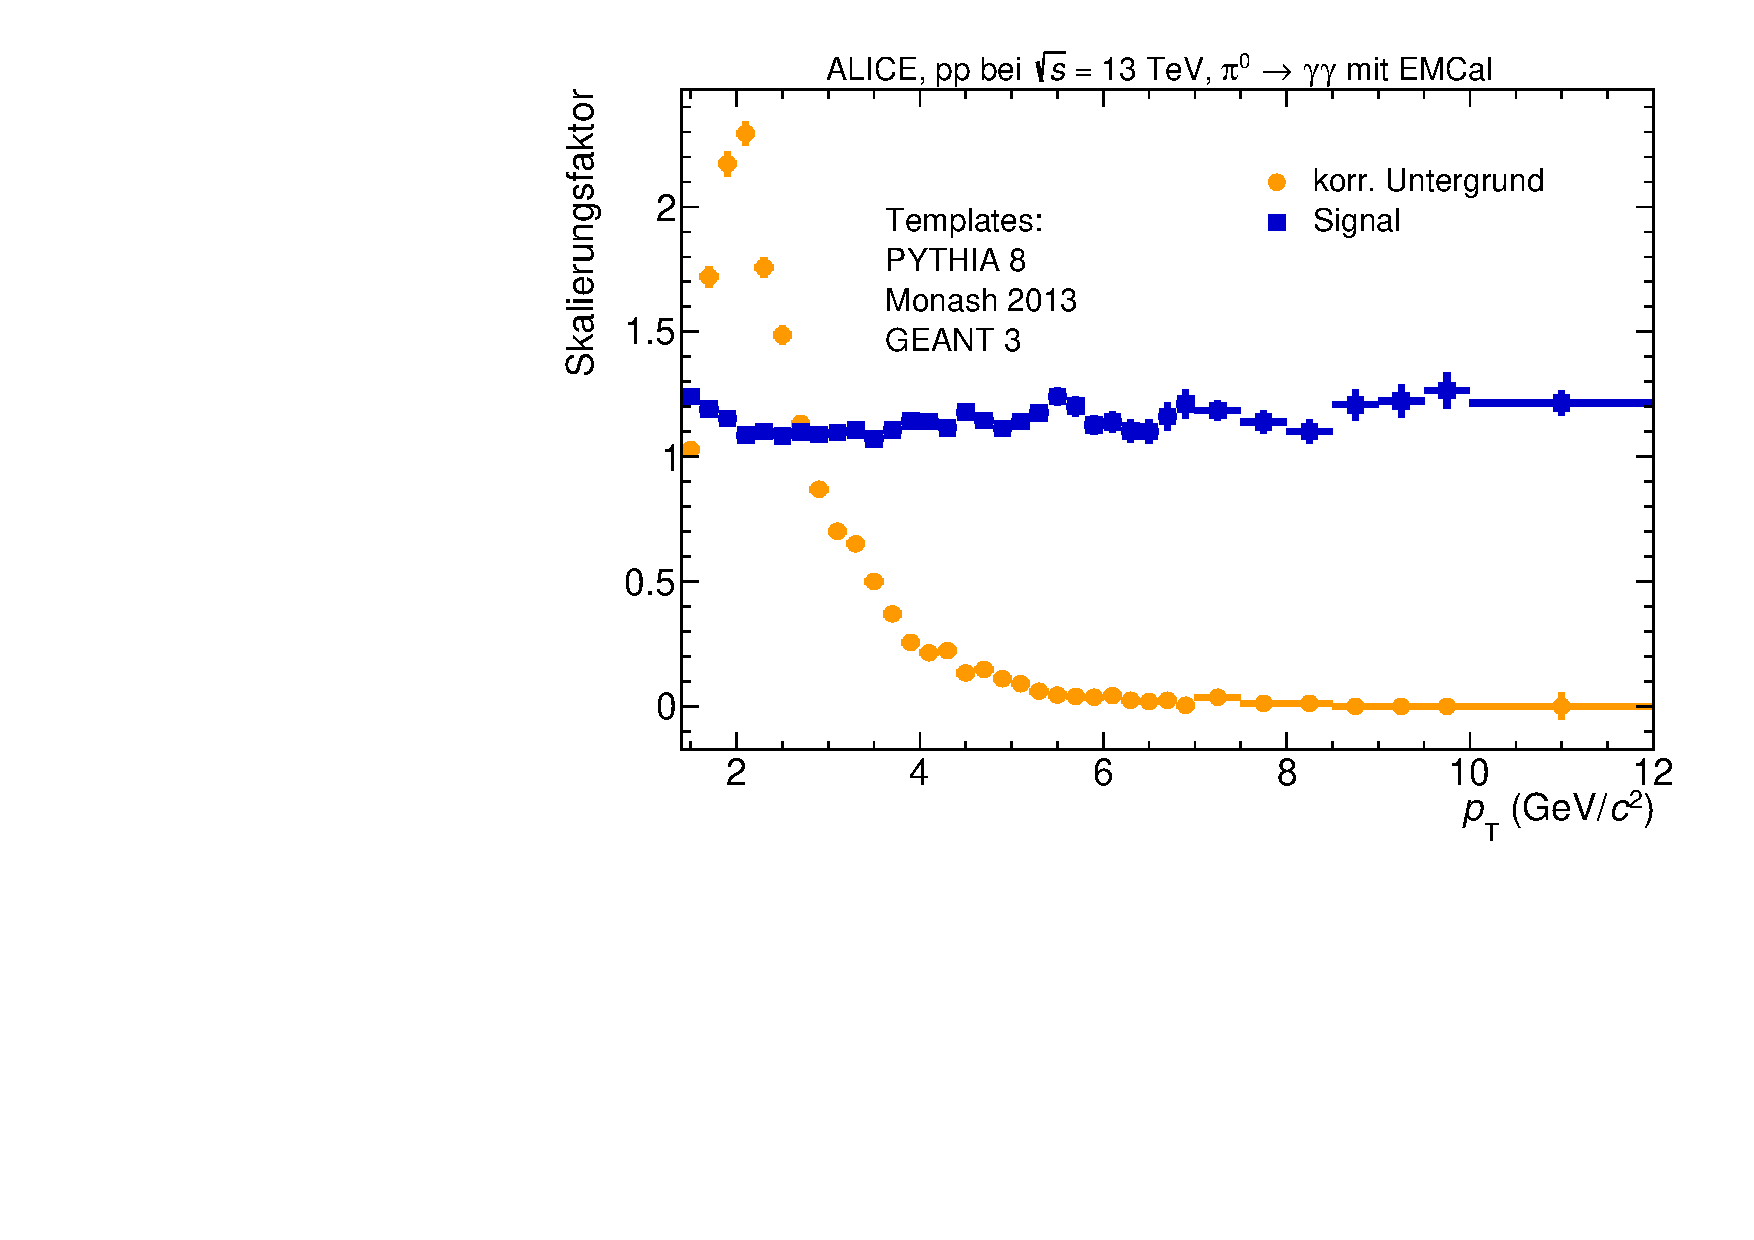
\includegraphics[width=.65\linewidth]{SF_Data_2016.pdf}
\caption{Skalierungsfaktoren der Templates des korrelierten Untergrunds und des Signals in Abhängigkeit von $p_{\text{T}}$.
}
\label{fig:SF}
\end{figure}
\newline
Die Skalierungsfaktoren aus die aus der $\chi^{2}$-Minimierung folgen werden in Abbildung \ref{fig:SF} gezeigt.
Für SF\textsubscript{korr. Untergrund} zeigt sich ein Anstieg bis es sein Maximum bei $1\,8 \leq p_{\text{T}}/(\text{ GeV}/c) < 2\,0$ erreicht.
Vom Maximum aus fällt SF\textsubscript{korr. Untergrund} ab, bis runter zur Null.
Da für alle $p_{\text{T}}$-Intervall das gleiche Template des korrelierten Untergrunds verwendet wird, kann aus dem Verlauf von SF\textsubscript{korr. Untergrund} direkt auf die Menge an korrelierten Untergrund geschlossen werden.
So wird für große $p_{\text{T}}$ kaum bis gar kein korrelierter Untergrund erwartet.
\newline
Die Templates des Signals sind jedoch für jeden $p_{\text{T}}$-Intervall unterschiedlich.
Das annähernd konstante Verhalten von SF\textsubscript{Signal} zeigt entsprechend, dass die Produktionsrate von $\pi^{0}$ in der Simulation gleichmäßig gut die Produktionsrate von $\pi^{0}$ im Experiment beschreibt.

\subsection{Abzug des korrelierten Untergrunds und Integration des Signals} \label{s3s5s4}
\begin{figure}[t!]
\centering
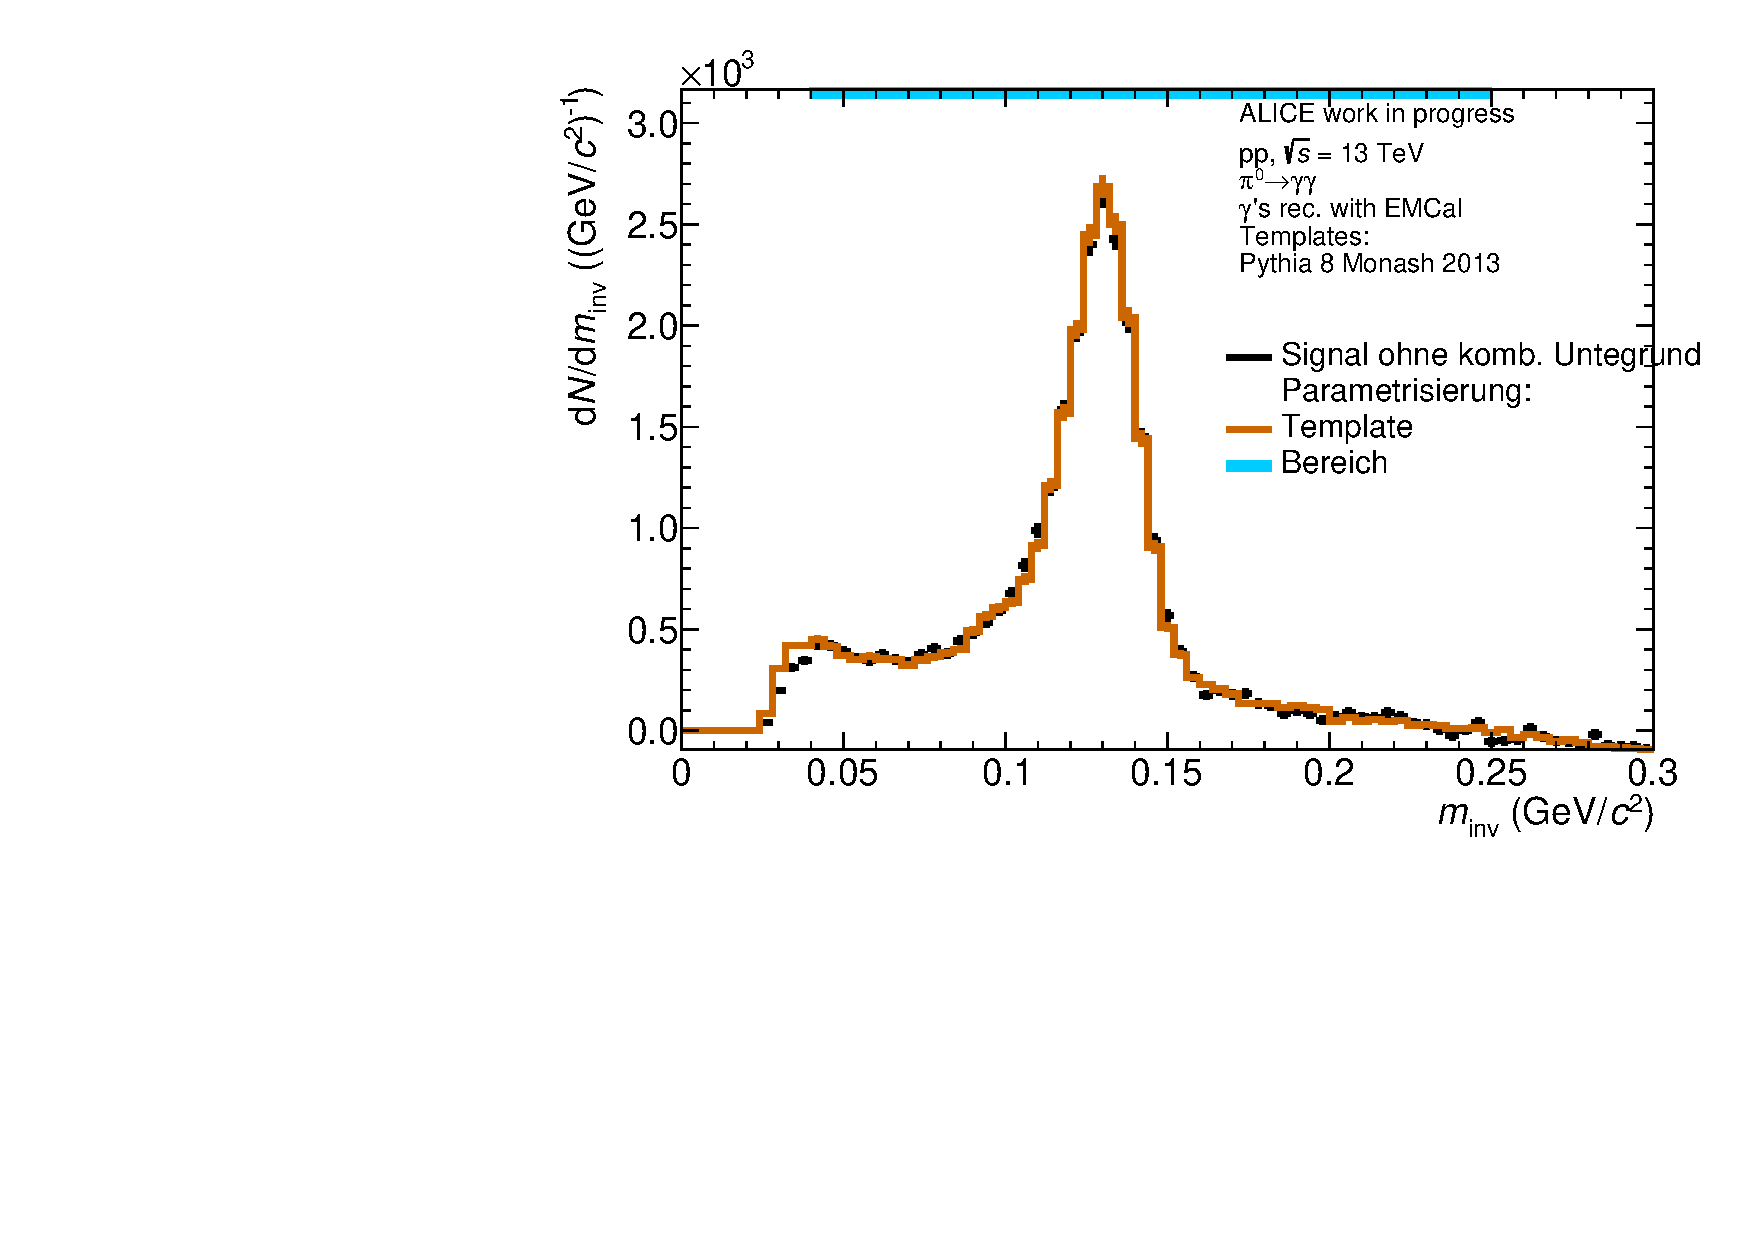
\includegraphics[width=.65\linewidth]{ParamResult_Bin10_Data_2016.pdf}
\caption{Signal mit unkorreliertem Untergrund zusammen mit Parametrisierung der Templates des korrelierten Untergrund und des Signals.
}
\label{fig:ParamResult}
\end{figure}
Das Ergebnis der Parametrisierung der Templates für das $p_\text{T}$-Intervall $(3\,2-3\,4)(\text{GeV/}c)$ wird in Abbildung \ref{fig:ParamResult} dargestellt.
Die Parametrisierung der beiden Templates stimmt innerhalb der Unsicherheiten gut mit den Daten überein, wie nach Abbildung \ref{fig:Chi2pT} zu erwarten war.
\newline
Um die Anzahl produzierter $\pi^{0}$ nun zu bestimmen, wird das skalierte Template des korrelierten Untergrunds von dem Signal ohne kombinatorischen Untergrund abgezogen.
Anschließend wird in einem bestimmten Zählbereich über die Werte des Signals summiert.
Dies wird für jedes $p_\text{T}$-Intervall durchgeführt.
\newline
Der Zählbereich hängt dabei von $p_\text{T}$ ab, da er so gewählt wurde, dass die untere Grenze immer groß genug ist, um nicht von den Anforderungen an den Öffnungswinkel betroffen zu sein.
Die obere Grenze liegt fest bei $p_\text{T} = 0\,25 \text{ GeV}/c$.
In Abbildung \ref{fig:ParamResult} wird er Zählbereich durch eine blaue Linie markiert.
\begin{figure}[t!]
\centering
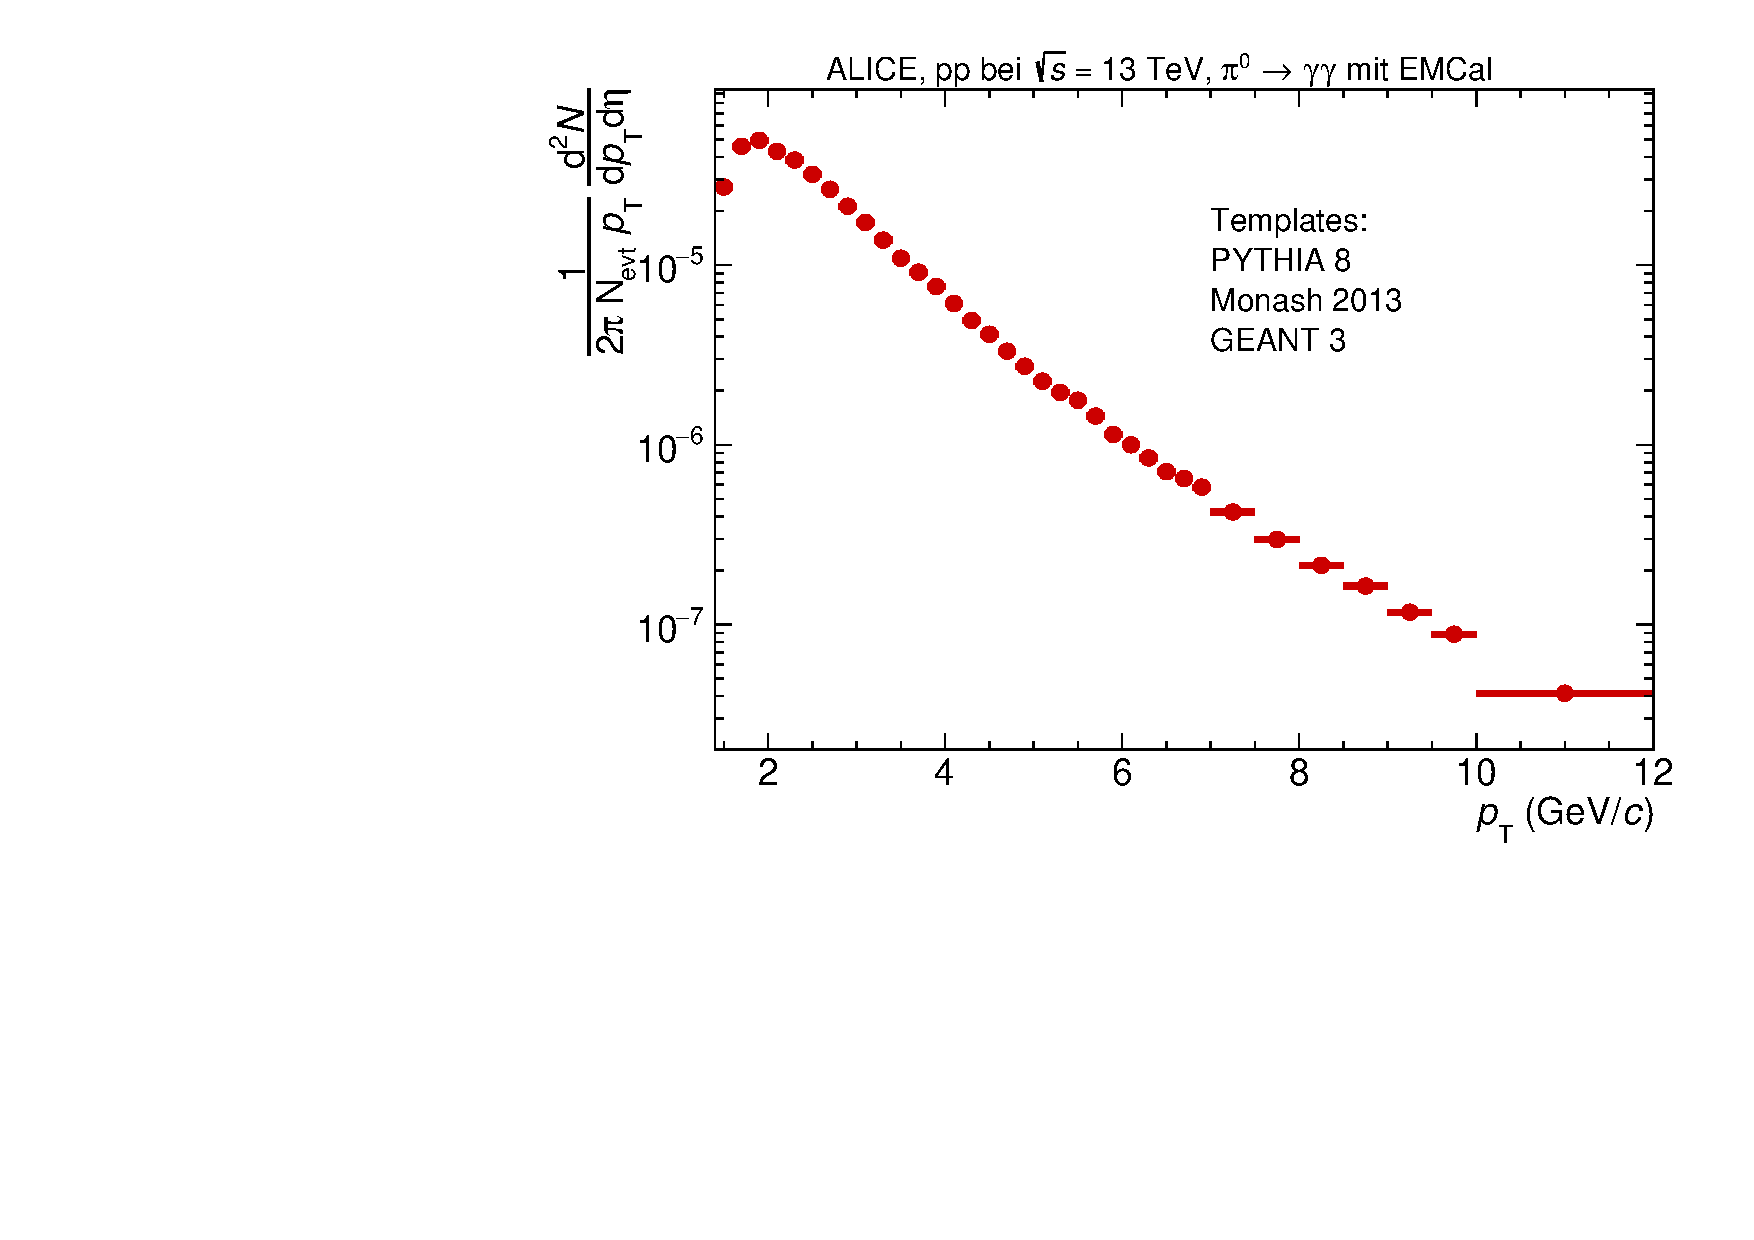
\includegraphics[width=.65\linewidth]{UncorrYields_Data_2016.pdf}
\caption{Anzahl rekonstruierter $\pi^{0}$ in Abhängigkeit von $p_\text{T}$.
}
\label{fig:RawYield}
\end{figure}
\newline
Das so erhaltene rohe Spektrum wird zusätzlich noch auf die Anzahl an \textit{events} $N_\text{evt}$, den Pseudorapiditätsbereich $\eta$, den Transversalimpuls $p_\text{T}$, die Wahrscheinlichkeit, dass ein $\pi^{0}$ in zwei Photonen zerfällt und $2\pi$ normiert.
Letzteres ist reine Konvention, während die anderen Normierungen einen Vergleich zwischen unterschiedlichen Analysen ermöglichen.
Abbildung \ref{fig:RawYield} zeigt das normierte rohe Spektrum.
Das Spektrum steigt zunächst leicht an, bis es bei $1\,8 \leq p_{\text{T}}/(\text{ GeV}/c) < 2\,0$ sein Maximum erreicht.
Danach sinkt das Spektrum kontinuierlich.
\newline
Für eine Aussage über die Produktionsrate von $\pi^{0}$ sowie einen allgemeinen Vergleich wird allerdings noch die Korrektur auf die Detektorakzeptanz sowie die Rekonstruktionseffizienz benötigt.

\chapter{Korrigierter Yield} \label{s4}

\section{Akzeptanz und Effizienz} \label{s4s1}
Die Korrekturen die auf das rohe Spektrum angewandt werden basieren auf der Monte Carlo Simulation, aus der auch die Templates für diese Analyse stammen.
\newline
Die Detektorakzeptanz spiegelt dabei die räumliche Abdeckung des EMCals wider.
Sie berechnet sich aus dem Verhältnis der \textit{Clusterpaare}, die auf das EMCal treffen, zu den produzierten \textit{Clusterpaaren}.
\newline
Die Effizienz berechnet sich aus der Division der \textit{Clusterpaare} aus dem Template des Signals durch die Anzahl der akzeptierten \textit{Clusterpaaren}.
Für die Effizienz wird der $m_\text{inv}$ Bereich zum Zählen benutzt, der auch für die Bestimmung des rohen Spektrums benutzt wurde.
\begin{figure}[t] %kein t!
\centering
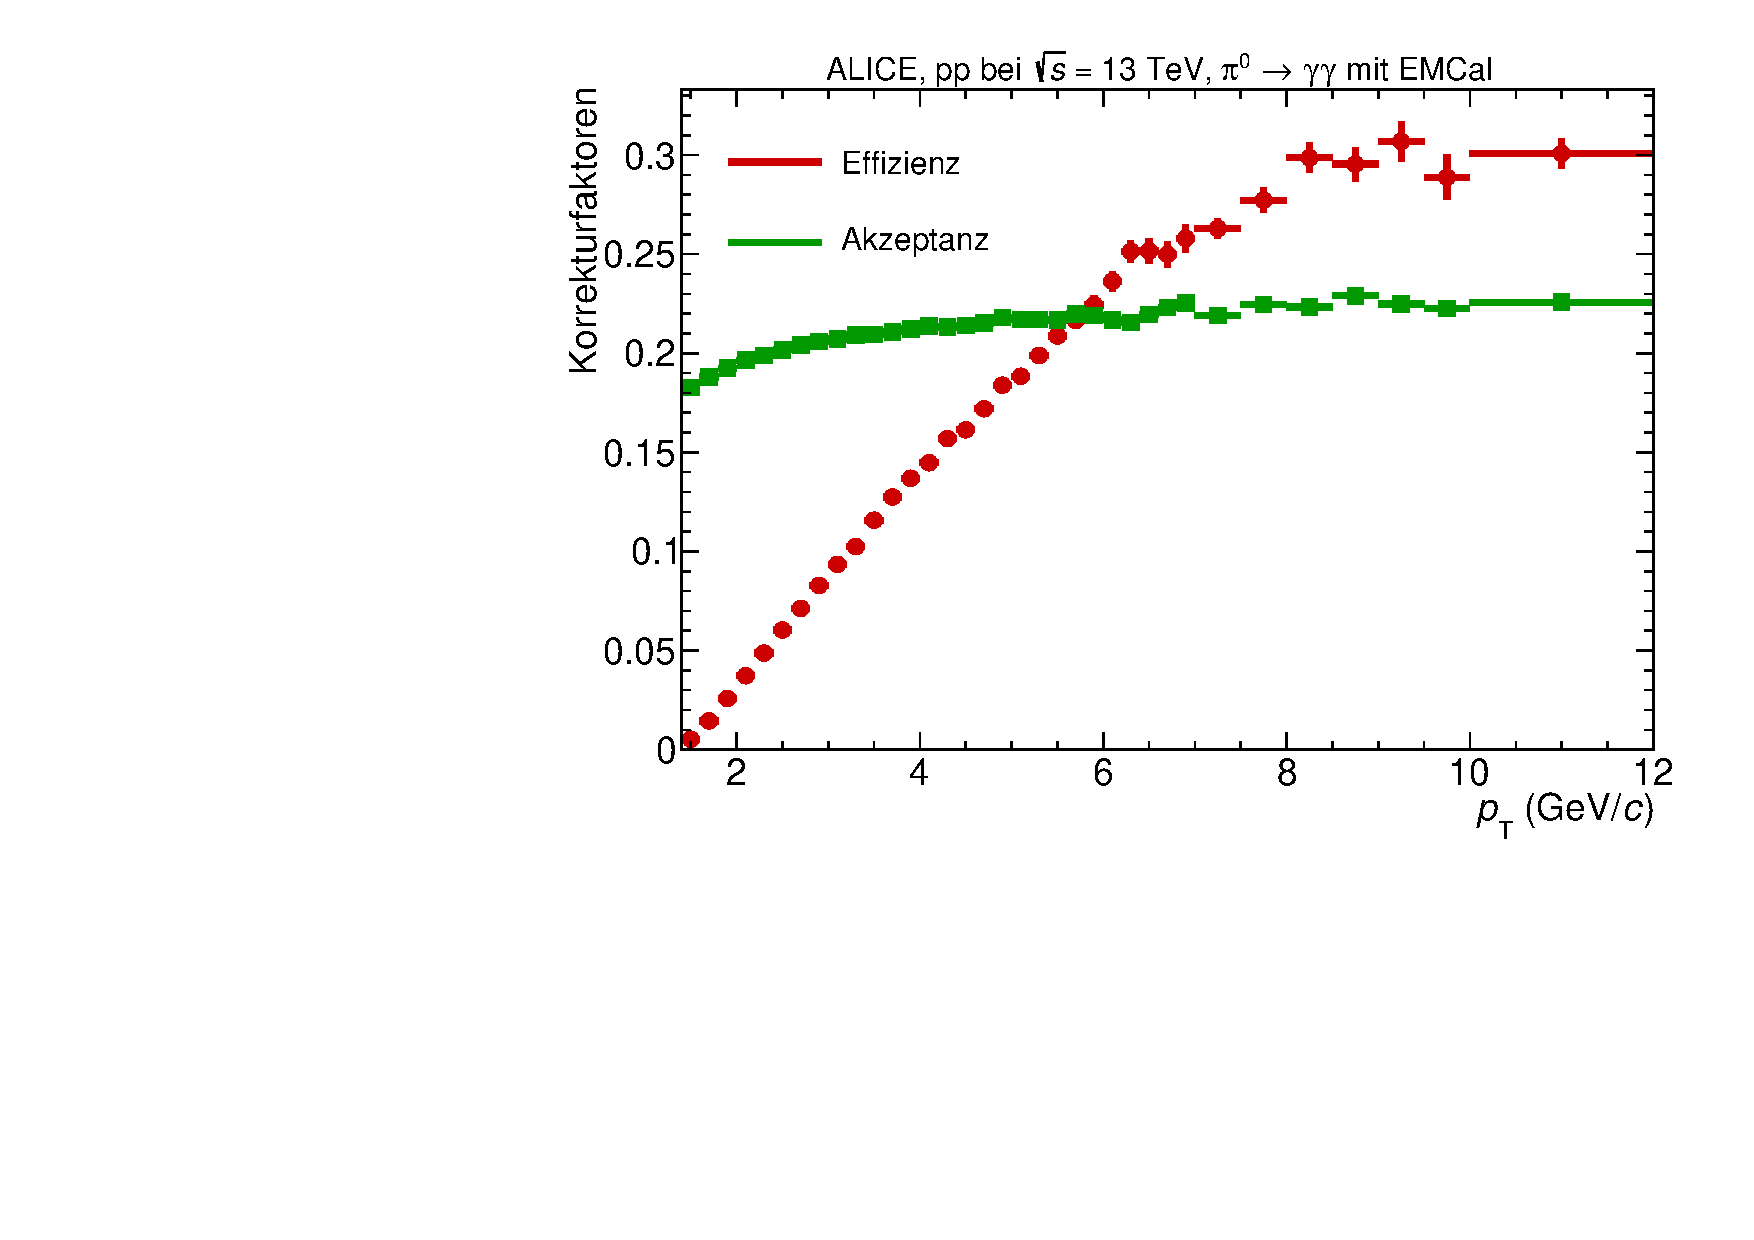
\includegraphics[width=.65\linewidth]{Korrekturfaktoren_Data_2016.pdf}
\caption{Detektorakzeptanz und Effizienz in Abhängigkeit von $p_\text{T}$.
}
\label{fig:Korrekturen}
\end{figure}
\newline
Durch das Korrigieren des rohen Spektrums mit der Detektorakzeptanz und der Effizienz, wird die Anzahl der detektierten und extrahierten $\pi^{0}$ auf die Anzahl der produzierten $\pi^{0}$ korrigiert.
Abbildung \ref{fig:Korrekturen} zeigt die beiden Korrekturgrößen Detektorakzeptanz und Effizienz.
\newline
Die Detektorakzeptanz wird mit steigendem $p_\text{T}$ größer.
Zerfällt ein $\pi^{0}$ in zwei Photonen, so fliegen die Photonen im System des $\pi^{0}$ entgegengesetzt zu einander weg, $\theta_{\gamma\gamma}$ beträgt in diesem System $180^{\circ}$.
Abhängig vom $p_\text{T}$ den ein $\pi^{0}$ im Laborsystem hat verringert sich $\theta_{\gamma\gamma}$.
Je größer $p_\text{T}$ umso kleiner $\theta_{\gamma\gamma}$ im Mittel.
Deshalb treffen beide Photonen aus einem $\pi^{0}$-Zerfall bei niedrigem $p_\text{T}$ seltener auf das EMCal.
Aus diesem Grund steigt die Detektorakzeptanz leicht an.
\newline
Durch die Anforderungen an die \textit{Cluster} werden unter anderem auch \textit{Cluster} ausgeschlossen, deren zugrunde liegende Teilchen aus dem Zerfall eines $\pi^{0}$ stammen, aber beispielsweise zu wenig Energie besitzen.
Gerade asymmetrische Zerfälle, bei denen der Anteil der zur Verfügung stehenden Energie ungleichmäßig auf die Zerfallsprodukte aufgeteilt wird, werden durch die Energieanforderung an die \textit{Cluster} ausgeschlossen.
Deshalb steigt die Effizienz bis $p_\text{T} = 8 \text{ GeV}/c$ an und saturiert dann.
Im Saturationsbereich werden immer mehr \textit{Cluster} zusammengefasst, da sie zu nah aneinander liegen.
Dadurch alleine würde die Effizienz wieder sinken, jedoch liegt der vorher genannte Effekt in diesem Bereich auch vor, wodurch die Saturation entsteht.
\begin{figure}[t!]
\centering
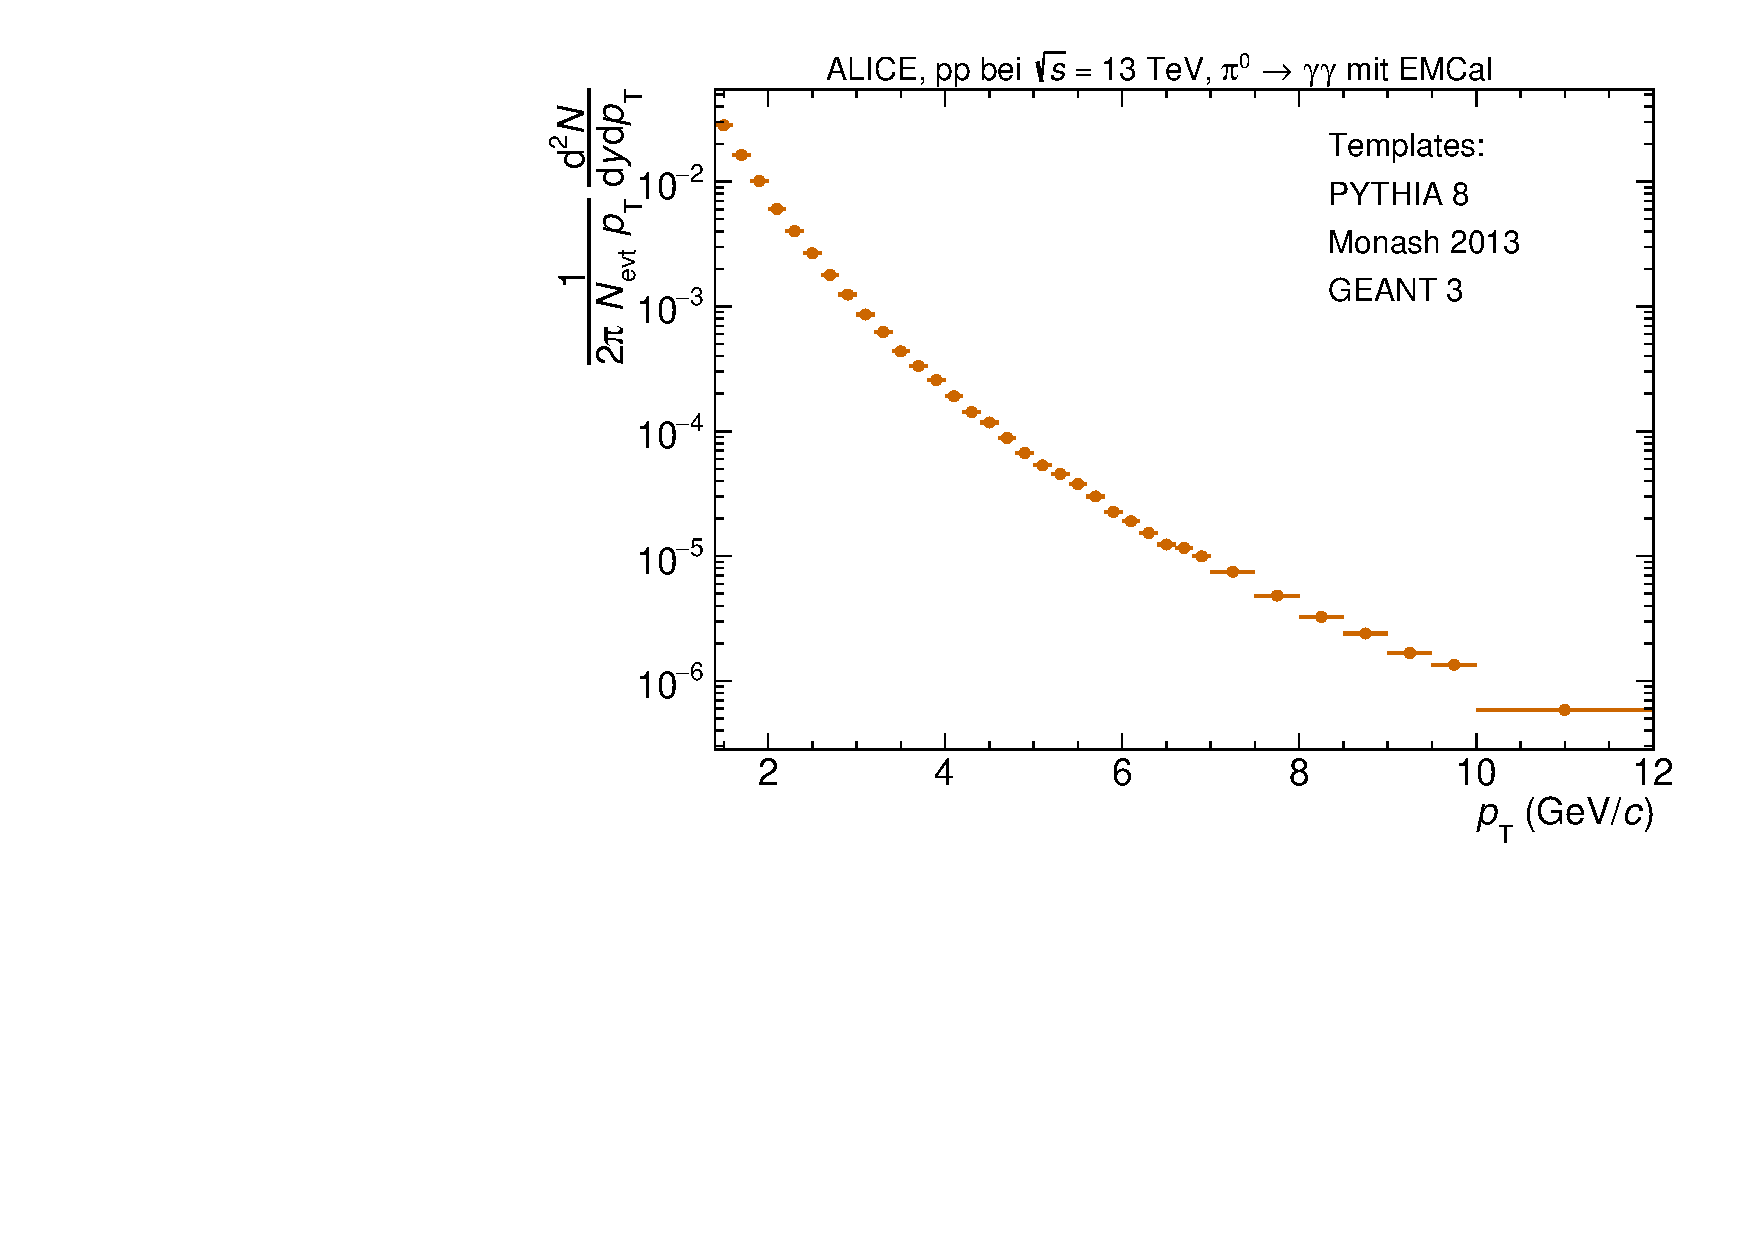
\includegraphics[width=.65\linewidth]{KorrigierterYieldNurStat_Data_2016.pdf}
\caption{Korrigiertes $p_\text{T}$-Spektrum mit statistischer Unsicherheit.
}
\label{fig:YieldStatUncer}
\end{figure}
\newline
Abbildung \ref{fig:YieldStatUncer} zeigt das korrigierte $p_\text{T}$-Spektrum mit statistischer Unsicherheit.
Ausgehend von dem korrigierten $p_\text{T}$-Spektrum wird im folgenden Abschnitt die systematische Unsicherheit für dieses bestimmt.

\section{Systematische Unsicherheit} \label{s4s2}
Für das korrigierte $p_\text{T}$-Spektrum wird zuletzt noch die systematische Unsicherheit bestimmt.
Dabei wird sich in dieser Arbeit rein auf die systematische Unsicherheit, die durch Variation in der Peakextraktion kommt, fokussiert.
Das korrigierte $p_\text{T}$-Spektrum, das mit der Variation extrahiert wurde, wird mit dem korrigierten $p_\text{T}$-Spektrum ohne Variationen verglichen.
Die Variationen die in dieser Arbeit verwendet wurden lassen sich in vier Abschnitte unterteilen.
\newline
Bei der \textbf{Variation des Zählbereiches} und der \textbf{Variation des Parametrisierungsbereiches}, wird der Zähl- beziehungsweise Parametrisierungsbereich einmal ausgeweitet und ein anderes mal verkleinert.
Bei der Variation wird die untere Grenze jeweils um $0,01 \text{ GeV}/c^{2}$ verschoben, während die obere Grenze um $0,025 \text{ GeV}/c^{2}$ verändert wird, wie Tabelle \ref{tab:ParamAndIntRange} zeigt.
Die Änderung der unteren Grenze wurde so gewählt, dass das kombinierte Template des korrelierten Untergrunds die einzelnen Templates trotz der Anforderung an den Öffnungswinkel gut beschreibt.
Gleichzeitig wird sicher gestellt, dass der Teil des Signals, der aus Konversionselektronen oder Konversionspositronen besteht, möglichst vollständig im Zähl- beziehungsweise Parametrisierungsbereich liegt.
\begin{table}[b!]
\centering
\begin{tabular}{c|c||c||c|}
\cline{2-4}
                                                                      & Standard & Vergr{\"o}{\ss}ert & Verkleinert \\ \hline
\multicolumn{1}{|c|}{\multirow{2}{*}{$m_\text{inv}\text{ (GeV}/c)$}} & $0,06$   & $0,05$             & $0,07$      \\ \cline{2-4} 
\multicolumn{1}{|c|}{}                                                & $0,25$   & $0,275$            & $0,225$     \\ \hline
\end{tabular}
\caption{Obere und untere Grenze des Parametrisierungs- und Zählbereichs}
\label{tab:ParamAndIntRange}
\end{table}
\begin{figure}[t]
\centering
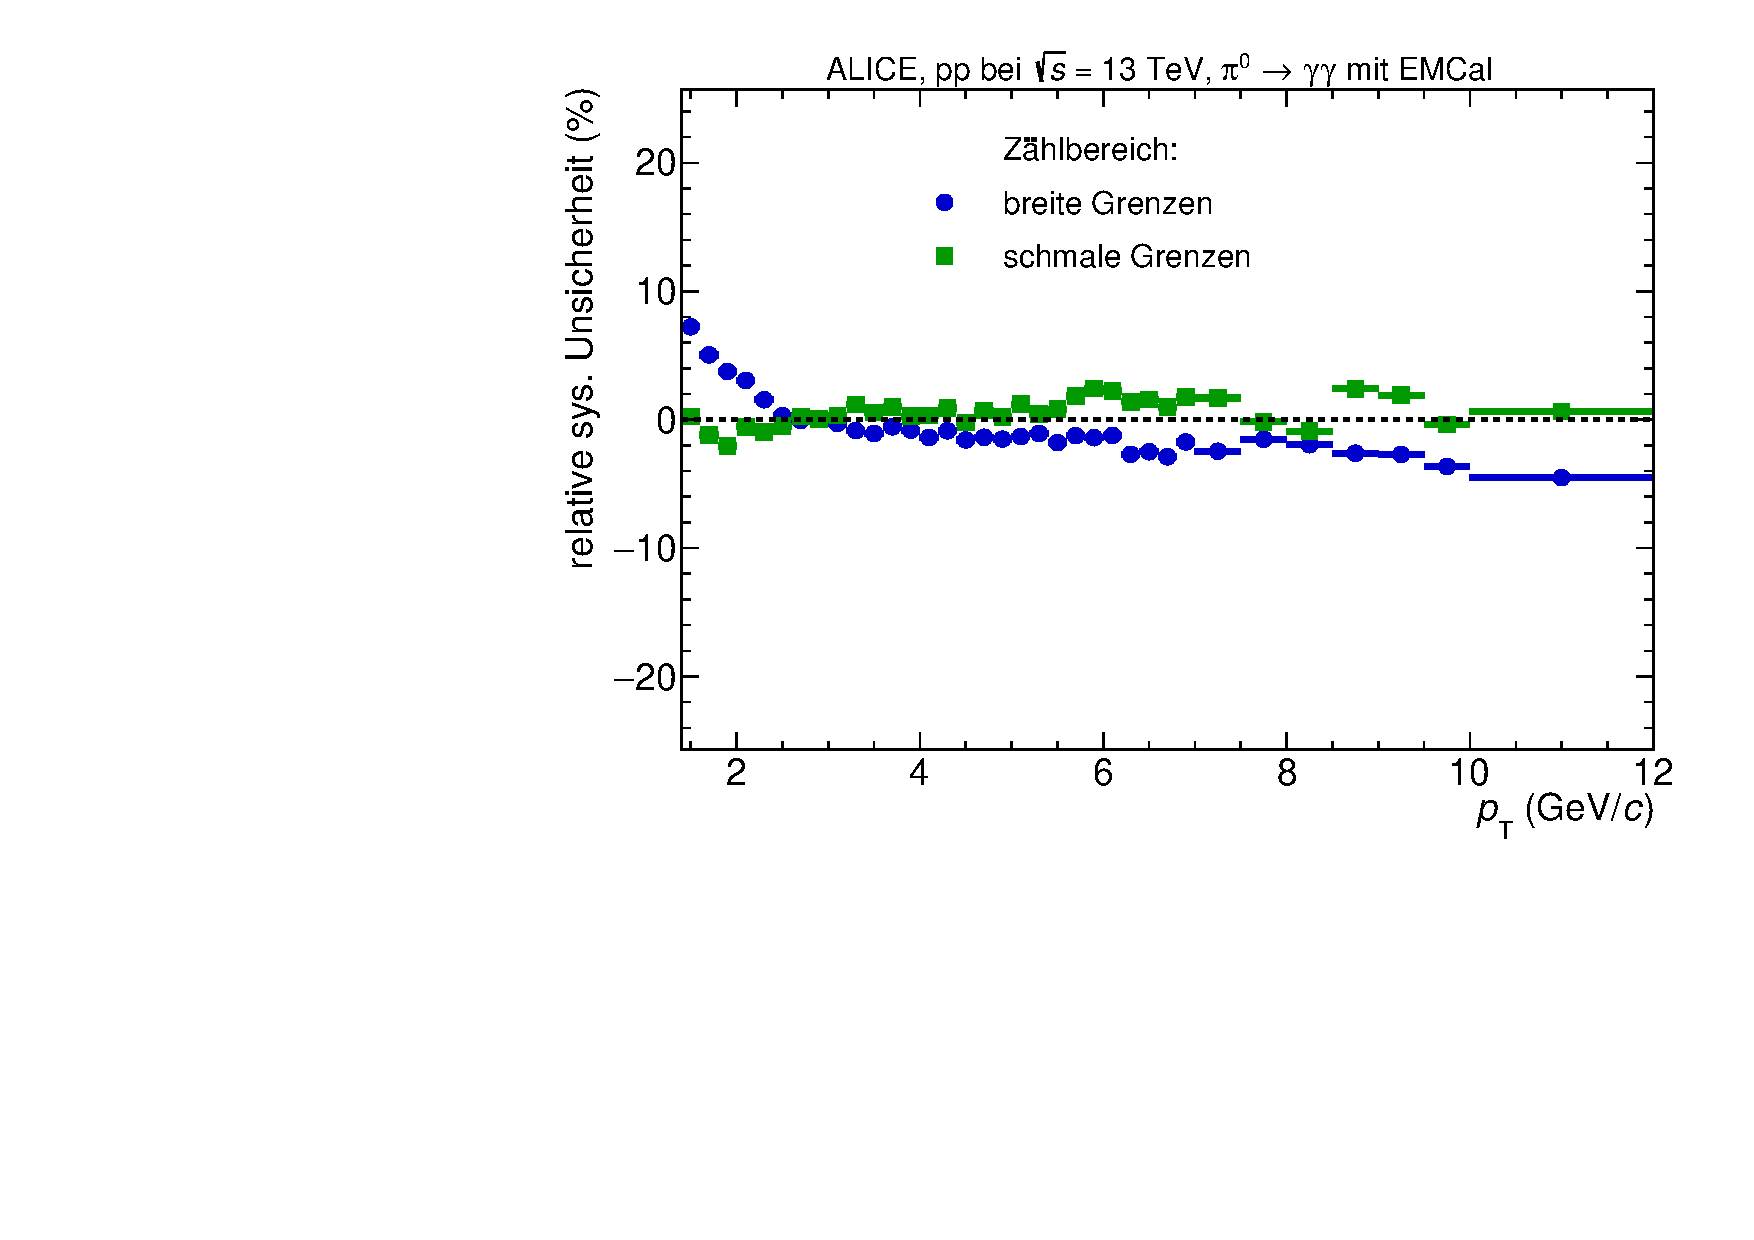
\includegraphics[width=.65\linewidth]{YieldsSysUncerIntRange_Data_2016.pdf}
\caption{Relative systematische Unsicherheit durch die Variation des Zählbereiches in Abhängigkeit von $p_\text{T}$.}
\label{fig:IntSys}
\end{figure}
\newline
Abbildung \ref{fig:IntSys} zeigt die relative systematische Abweichung für die Variation des Zählbereiches.
Beide Variationen weisen eine lineare Abweichung auf.
Die Abweichungen für breite Grenzen liegt ab $p_\text{T} > 5,8 \text{ GeV}/c$ im positiven Bereich, während die Abweichungen für schmale Grenzen dort im negativen liegen.
\begin{figure}[t!]
\centering
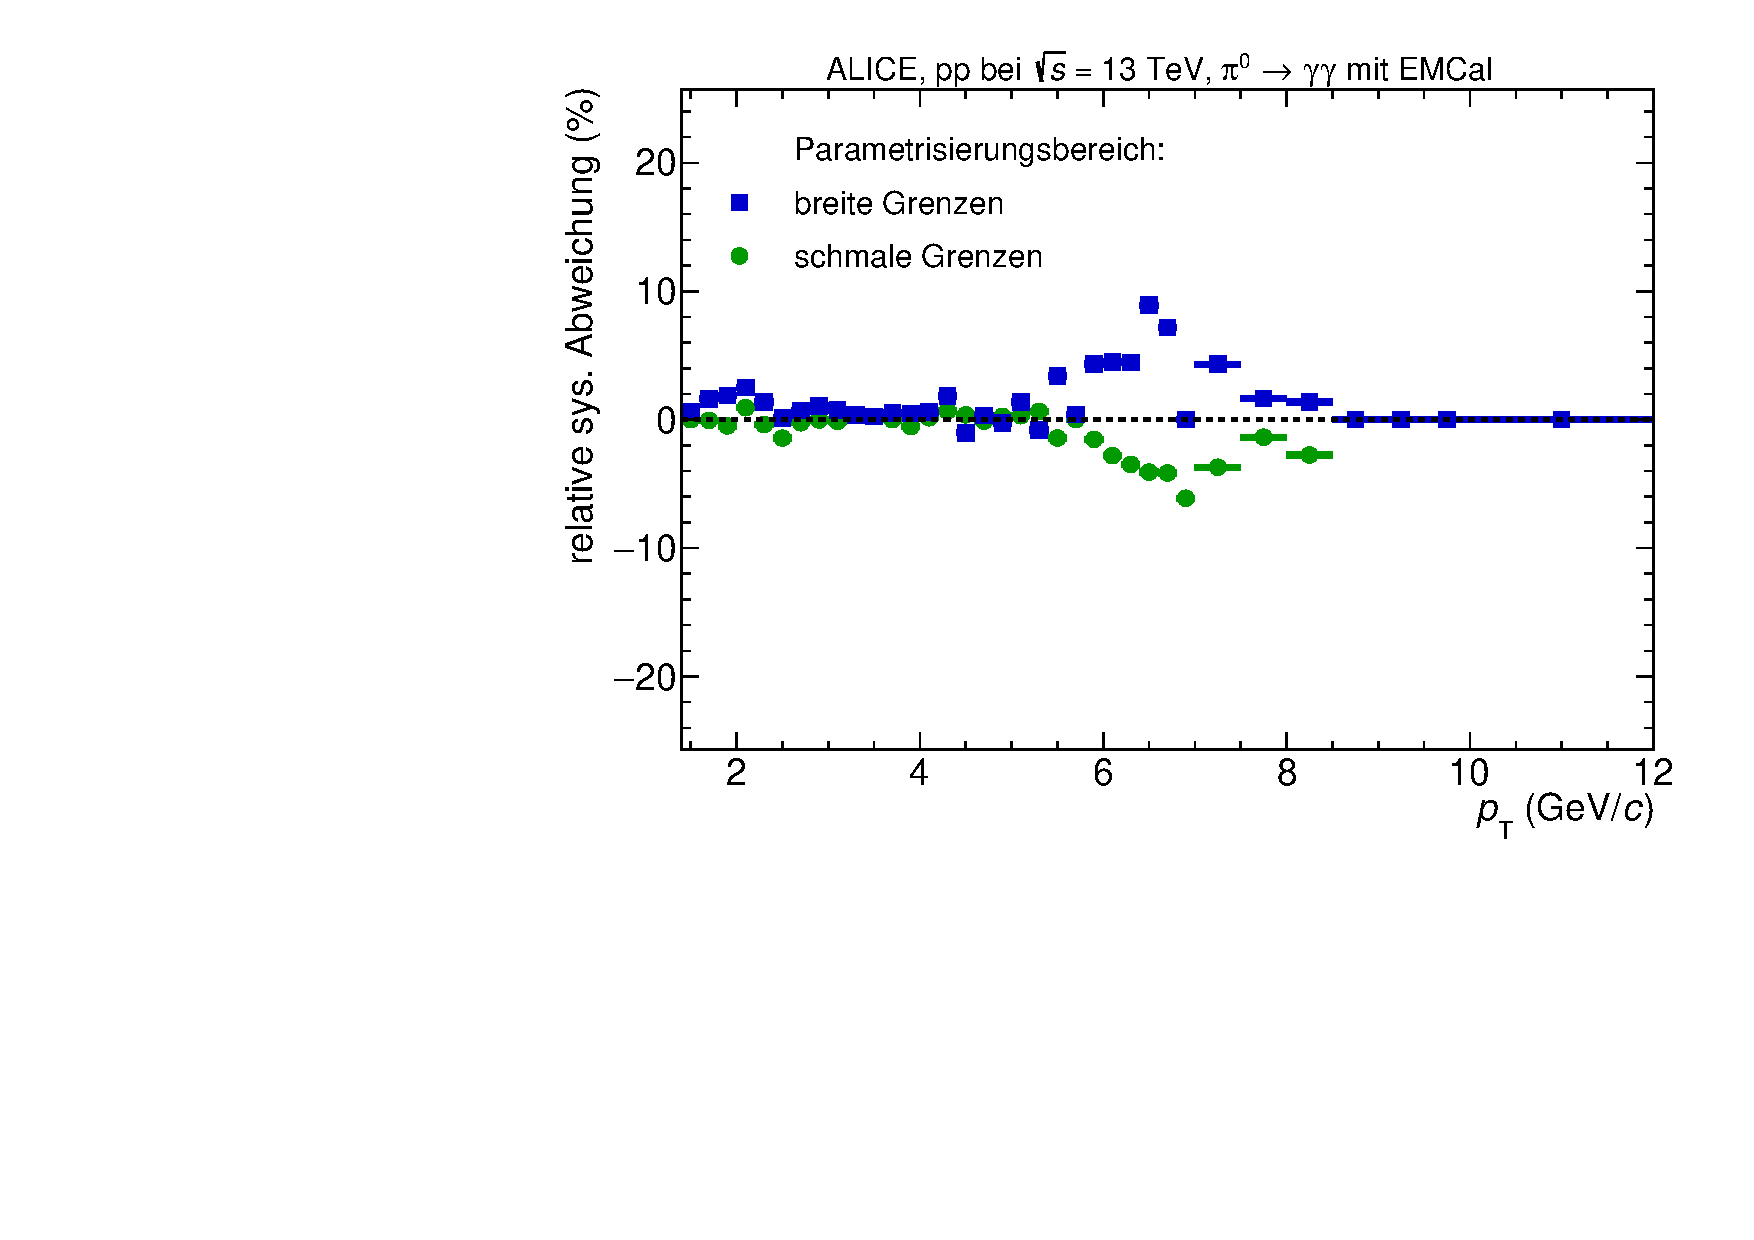
\includegraphics[width=.65\linewidth]{YieldsSysUncerFitRange_Data_2016.pdf}
\caption{Relative systematische Unsicherheit durch die Variation des Paramtrisierungsbereiches in Abhängigkeit von $p_\text{T}$.}
\label{fig:ParamSys}
\end{figure}
\newline
Abbildung \ref{fig:ParamSys} zeigt die relative systematische Unsicherheit für die Variation des Parametrisierungsbereiches.
Die Abweichungen befinden sich nahe der Null für schmale und breite Grenzen.
Eine Ausnahme bildet der $p_\text{T}$-Bereiches von $5,8 \text{ GeV}/c$ bis $7,5 \text{ GeV}/c$.
Dort liegen die Werte für breite Grenzen deutlich im positiven, die Werte für kleine Grenzen liegen hingegen im negativen Bereich.
\begin{figure}[t!]
\centering
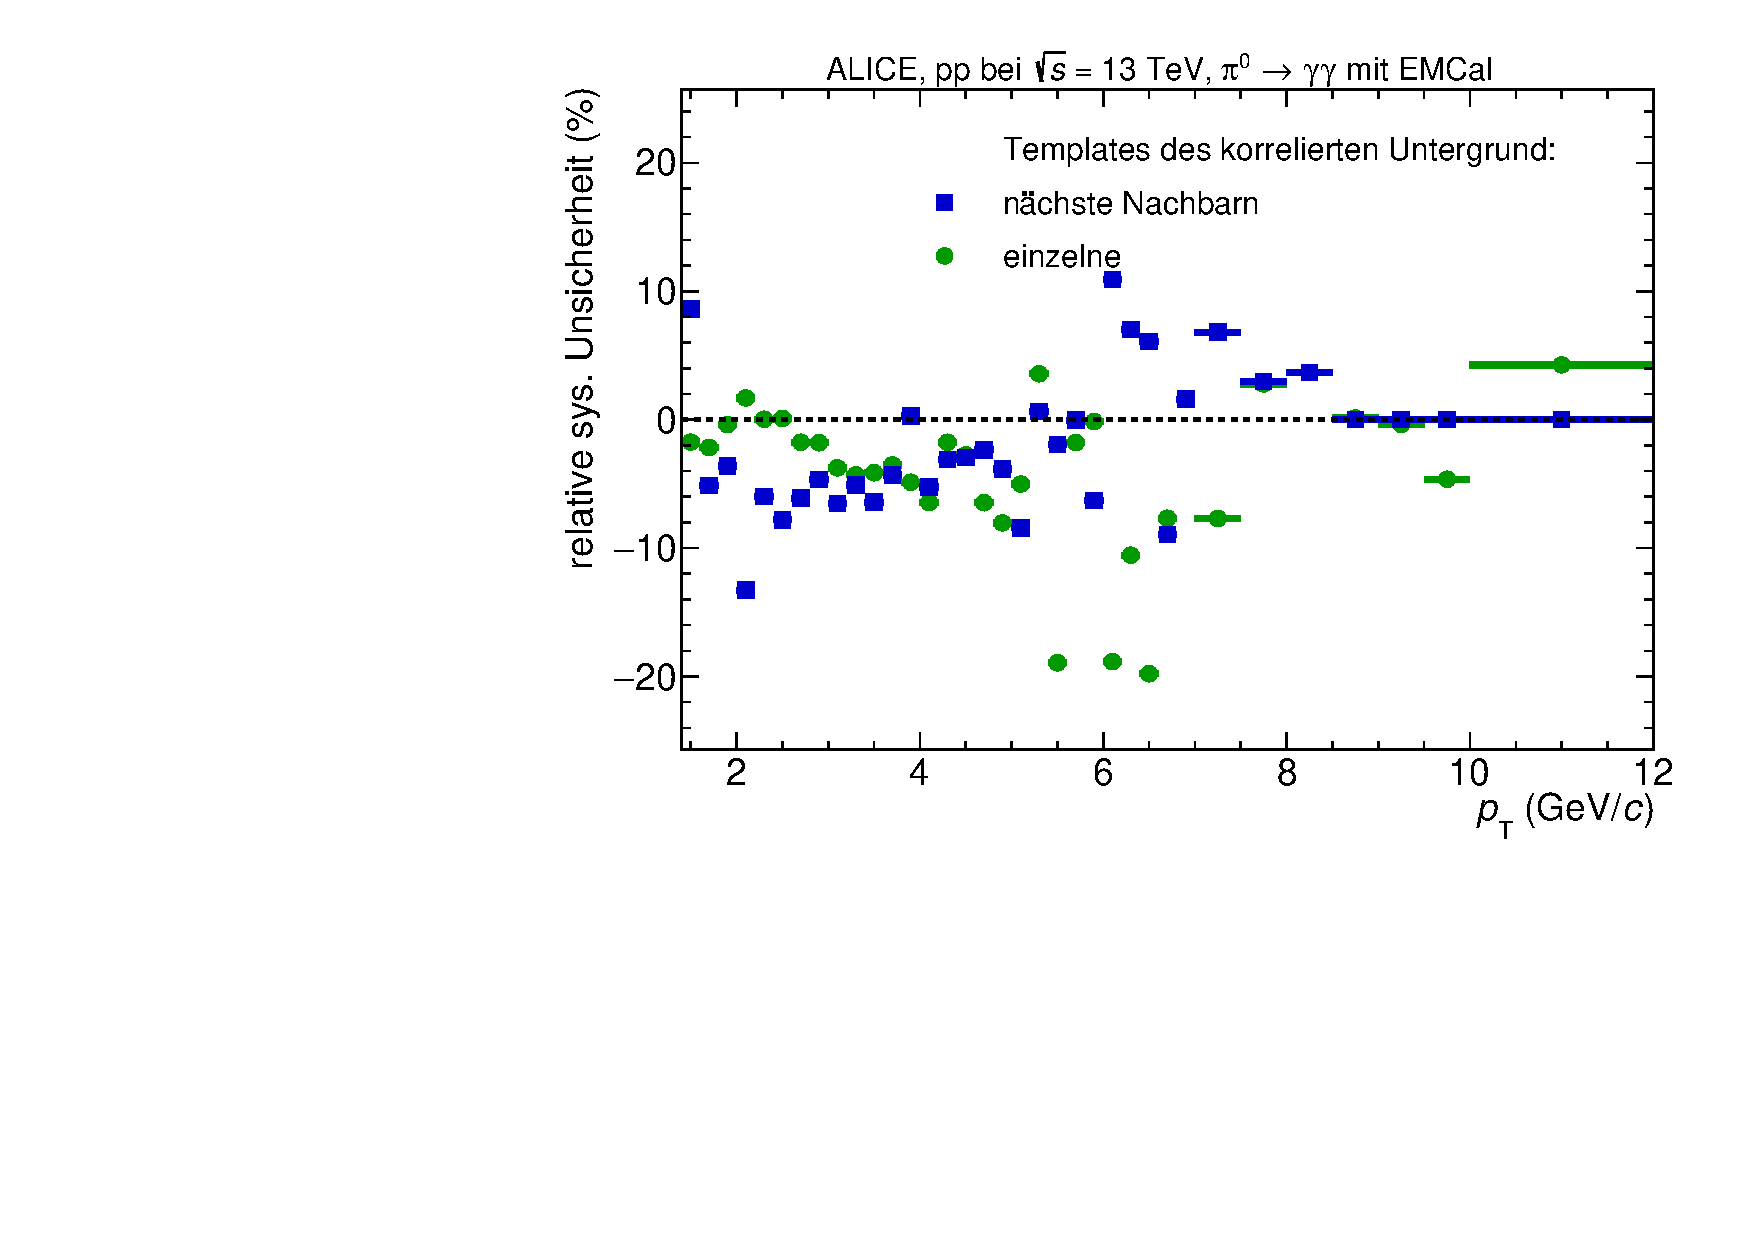
\includegraphics[width=.65\linewidth]{YieldsSysUncerBkgVariation_Data_2016.pdf}
\caption{Relative systematische Abweichung durch die Variation der Templates des korrelierten Untergrunds in Abhängigkeit von $p_\text{T}$.}
\label{fig:BkgSys}
\end{figure}
\newline
Die \textbf{Variation der Templates des korrelierten Untergrunds} basiert auf den in Abschnitt \ref{s3s5s2} vorgestellten Methoden zur Bestimmung der Templates des korrelierten Untergrunds.
Für kleine $p_\text{T}$ von $1,4 \text{ GeV}/c$ bis $4,4 \text{ GeV}/c$ zeigen beide Methoden eine geringe Abweichung.
Der $p_\text{T}$-Bereich von $4,4 \text{ GeV}/c$ bis $7,5 \text{ GeV}/c$ hingegen weist starke Abweichungen für beide Methoden auf.
Die Methode mit einzelnen Templates des korrelierten Untergrunds unterschätzt in diesem Bereich die Anzahl produzierter $\pi^{0}$ im Vergleich zur Methode mit kombiniertem Template des korrelierten Untergrunds stark.
Die Ursache hierfür liegt vor allem in der großen statischen Unsicherheit der einzelnen Templates des korrelierten Untergrunds.
Durch diese Unsicherheit wird der korrelierte Untergrund überschätzt.
Bei der Methode mit den nächsten Nachbarn wird der korrelierten Untergrund hingegen unterschätzt, weshalb dort die Abweichung im positiven Bereich liegt.
\begin{figure}[t!]
\centering
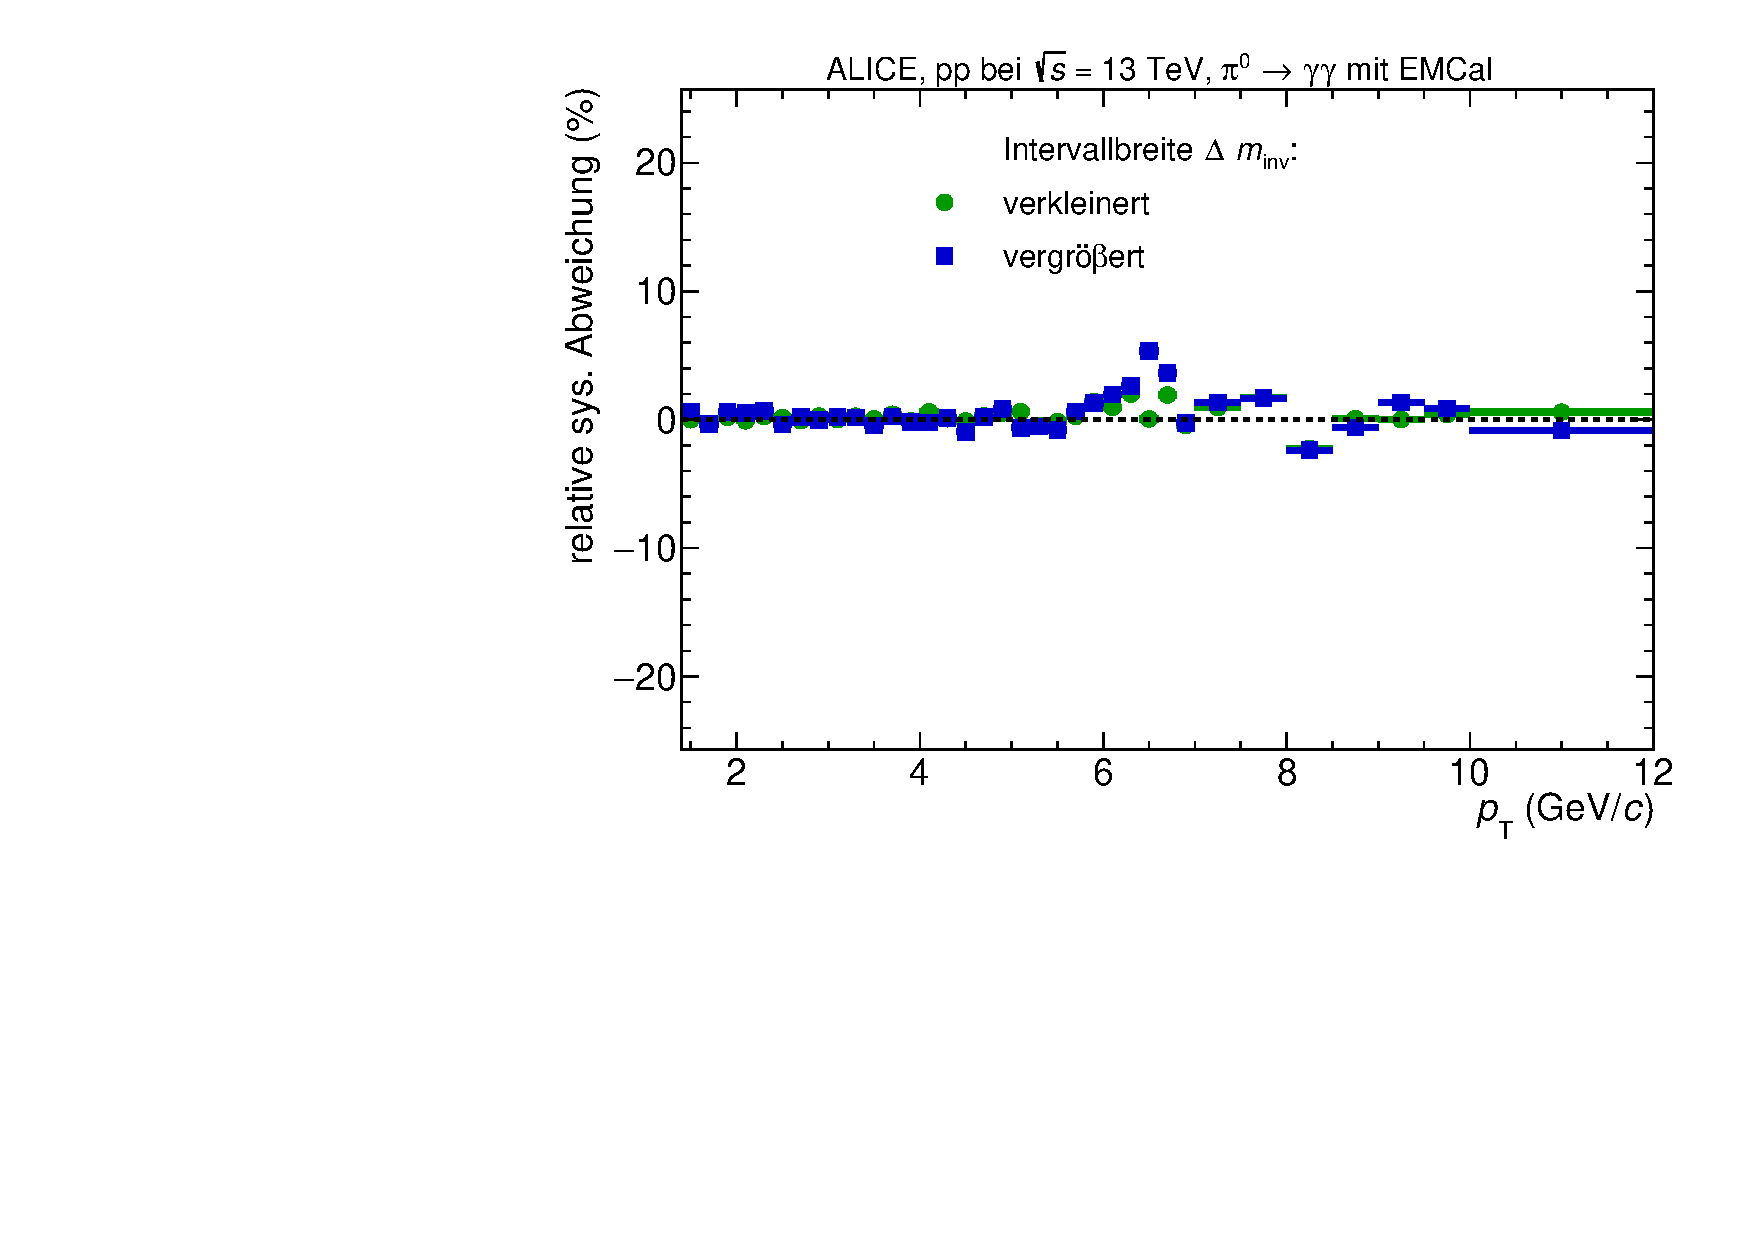
\includegraphics[width=.65\linewidth]{YieldsSysUncerRebinning_Data_2016.pdf}
\caption{Relative systematische Abweichung durch die Variation von $\Delta m_\text{inv}$ in Abhängigkeit von $p_\text{T}$.}
\label{fig:BinningSys}
\end{figure}
\newline
Die Breite der $m_\text{inv}$-Intervalle $\Delta m_\text{inv}$ wird in der \textbf{Variation von} $\boldsymbol{\Delta m}_\textbf{inv}$ verändert.
Tabelle \ref{tab:Binning} zeigt $\Delta m_\text{inv}$ wie es für diese Analyse gewählt wurde, sowie für die Variationen.
Dabei hängt $\Delta m_\text{inv}$ zusätzlich von $p_\text{T}$ ab.
\newline
Beide Variationen zeigen kaum Abweichungen, lediglich im $p_\text{T}$-Bereich von $6,0 \text{ GeV}/c$ bis $7,5 \text{ GeV}/c$ bildet sich eine deutliche Abweichung für vergrößerte $\Delta m_\text{inv}$ ab.
\begin{table}[b!]
\centering
\begin{tabular}{c|c|c|}
\cline{2-3}
                                                          & $\Delta m_\text{inv}$ $\left(\text{GeV}/c^{2}\right)$ & $p_\text{T}$-Intervall $\left(\text{GeV}/c\right)$ \\ \hline
\multicolumn{1}{|c|}{\multirow{3}{*}{Standard}}           & $0\,004$                                              & $1\,4-7\,5$                                        \\ \cline{2-3} 
\multicolumn{1}{|c|}{}                                    & $0\,008$                                              & $7\,5-10$                                          \\ \cline{2-3} 
\multicolumn{1}{|c|}{}                                    & $0\,010$                                              & $10-12$                                            \\ \hline \hline
\multicolumn{1}{|c|}{\multirow{3}{*}{Vergr{\"o}{\ss}ert}} & $0\,005$                                              & $1\,4-7\,5$                                        \\ \cline{2-3} 
\multicolumn{1}{|c|}{}                                    & $0\,010$                                              & $7\,5-10$                                          \\ \cline{2-3} 
\multicolumn{1}{|c|}{}                                    & $0\,020$                                              & $10-12$                                            \\ \hline \hline
\multicolumn{1}{|c|}{\multirow{3}{*}{Verkleinert}}        & $0\,002$                                              & $1\,4-7\,5$                                        \\ \cline{2-3} 
\multicolumn{1}{|c|}{}                                    & $0\,005$                                               & $7\,5-10$                                          \\ \cline{2-3} 
\multicolumn{1}{|c|}{}                                    & $0\,008$                                              & $10-12$                                            \\ \hline
\end{tabular}
\caption{Die verschiedenen Breiten der $m_\text{inv}$-Intervalle $\Delta m_\text{inv}$ in Abhängigkeit von $p_\text{T}$.}
\label{tab:Binning}
\end{table}
\begin{figure}[t!]
\centering
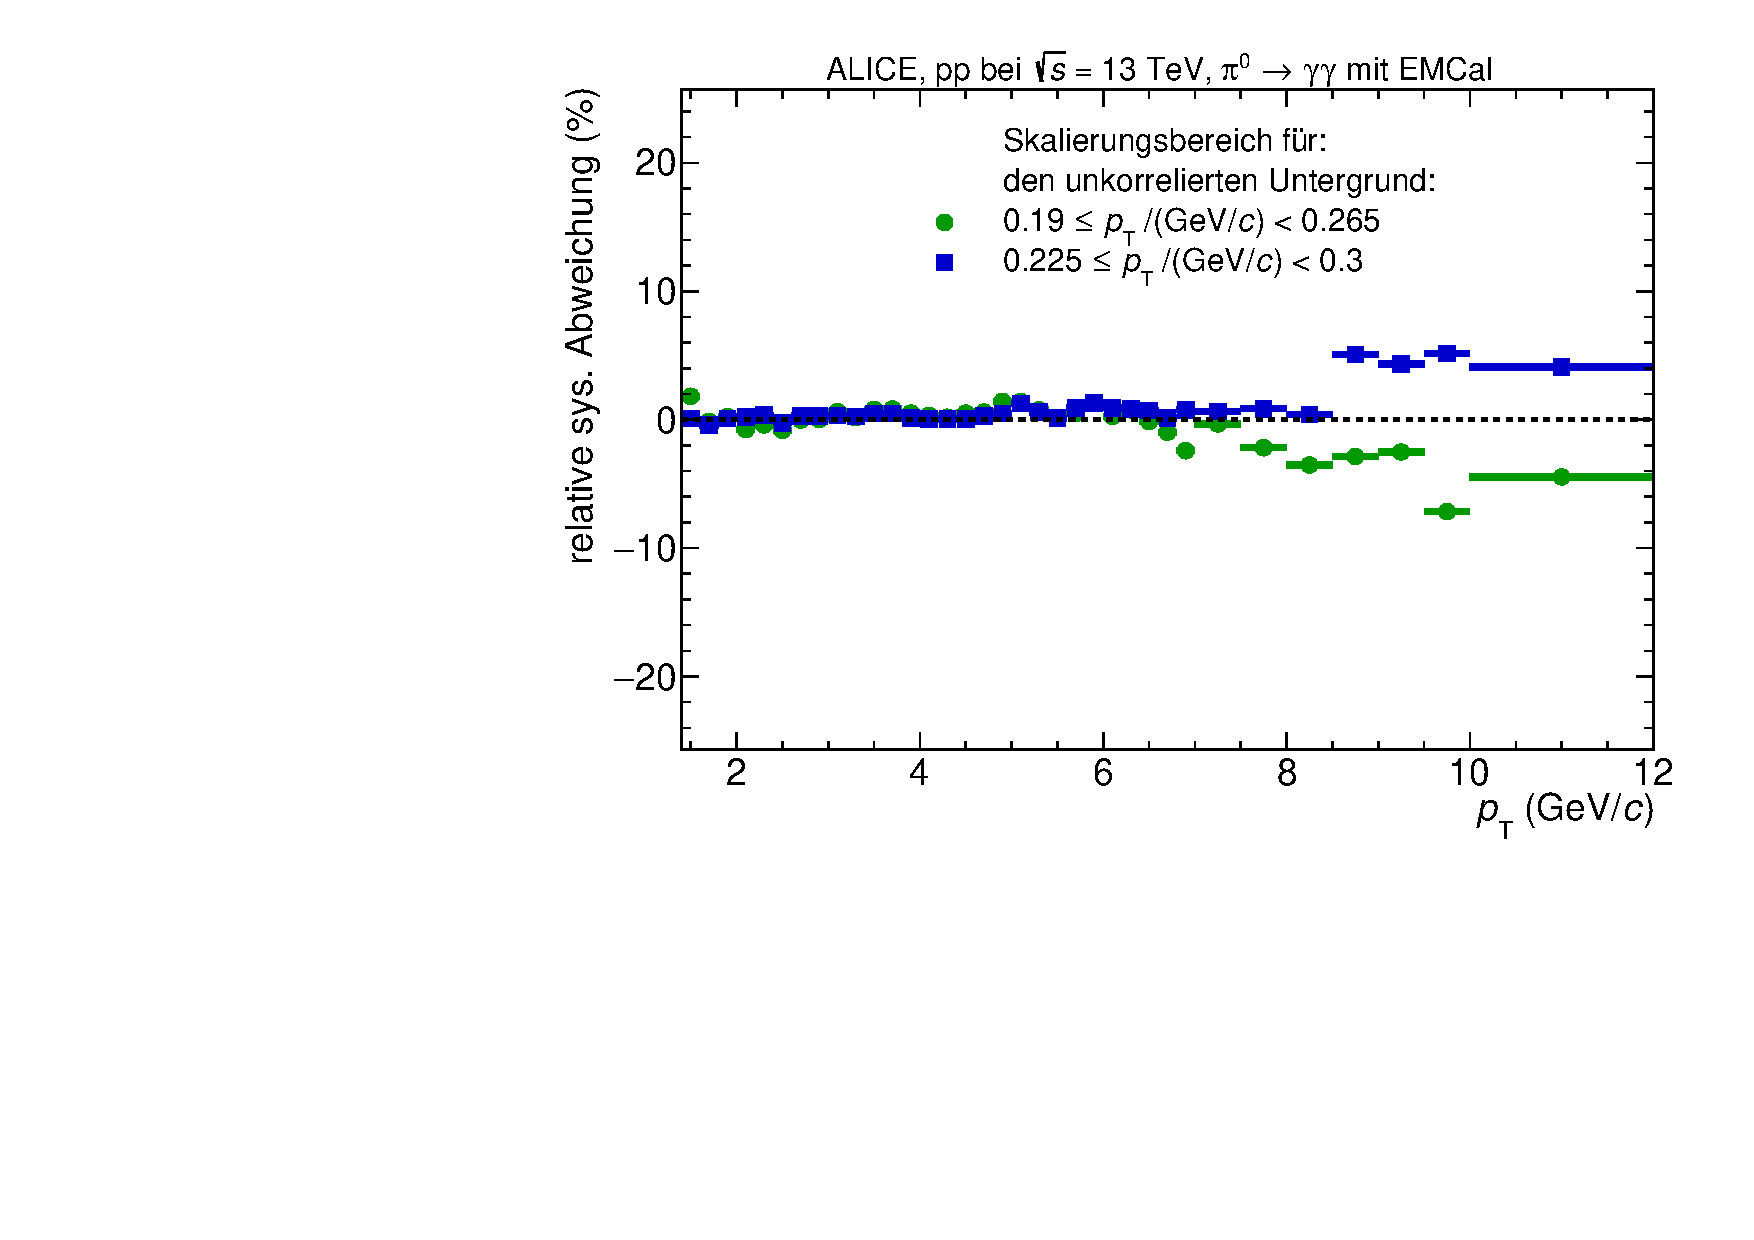
\includegraphics[width=.65\linewidth]{YieldsSysUncerUncorrBkgVariation_Data_2016.pdf}
\caption{Relative systematische Abweichung durch die Variation des Parametrisierungsbereiches des unkorrelierten Untergrunds in Abhängigkeit von $p_\text{T}$.}
\label{fig:LeftBkgSys}
\end{figure}
\newline
Bei der \textbf{Variation des Parametrisierungsbereiches des unkorrelierten Untergrunds} wird der Bereich verändert, indem die \textit{mixed Event} Verteilung skaliert wird.
Abbildung \ref{fig:LeftBkgSys} zeigt die zugehörigen Abweichungen.
Bis $p_\text{T} = 7,5 \text{ GeV}/c$ weisen beide Abweichungen einen linearen Verlauf um Null rum auf.
Ab $p_\text{T} = 7,5 \text{ GeV}/c$ weicht die Variation, bei der die obere Grenze nach unten verschoben wurde, ins negative ab.
Die Variation, bei der die untere Grenze verändert wurde, zeigt eine positive Abweichung, wobei diese erst ab $p_\text{T} = 8,5 \text{ GeV}/c$ auftritt.
\begin{figure}[t!]
\centering
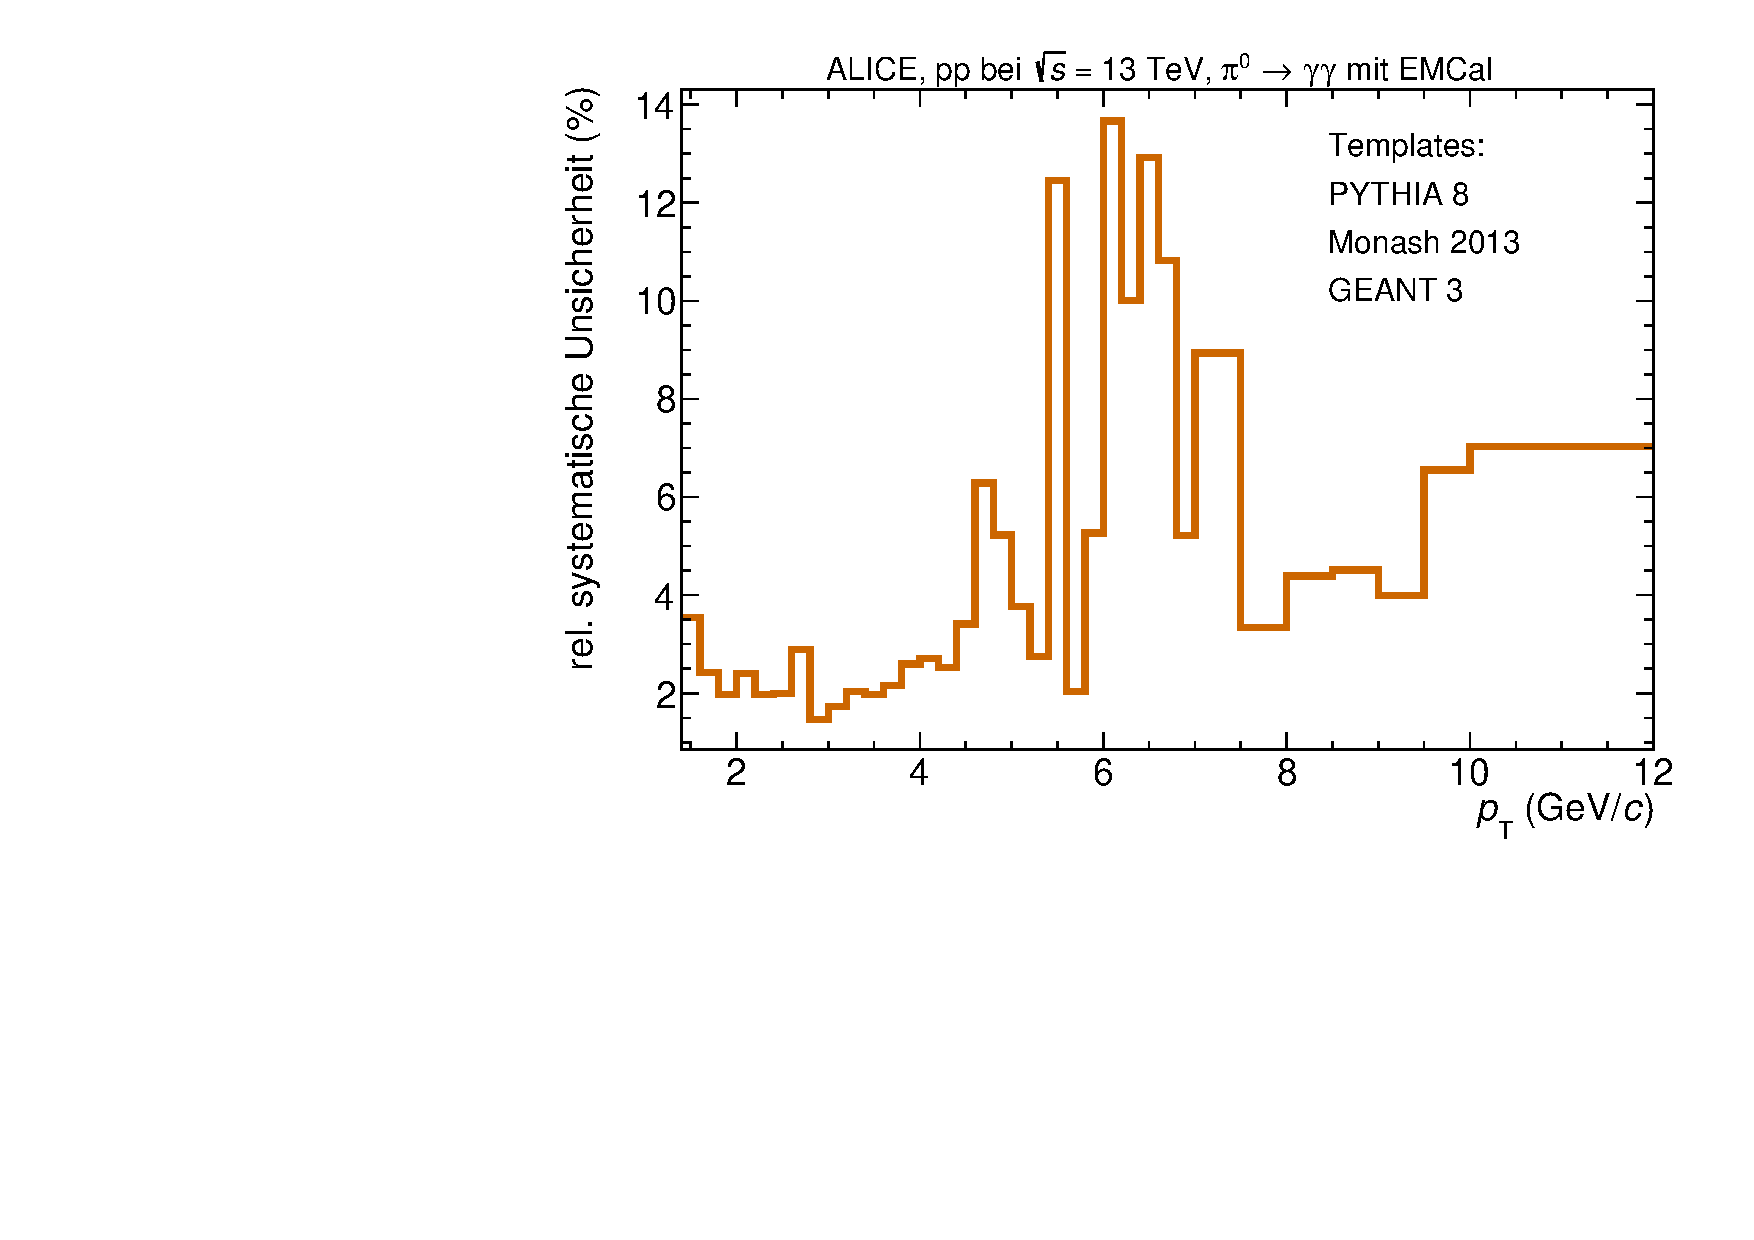
\includegraphics[width=.65\linewidth]{SystematischeUnsicherheit_Data_2016.pdf}
\caption{Gesamte relative systematische Unsicherheit des korrigierten $\pi^ {0}$-Spektrums.}
\label{fig:SysUncer}
\end{figure}
\newline
Zur Bestimmung der systematischen Unsicherheit $\sigma_{i,j}$ einer Variationsart $j$ in einem $p_\text{T}$-Intervall $i$ wird das quadratische Mittel der relativen Abweichungen der $n$ unterschiedlichen Variationen $k$ verwendet.
Es gilt:
\begin{align}
\sigma_{i,j} = \sqrt{\frac{1}{n}\sum_{k=1}^{n}\left(\Delta y_{i,j,k}\right)^{2}}
\end{align}
Die gesamte Systematische Unsicherheit $\sigma_{i}$ in einem $p_\text{T}$-Intervall $i$ ergibt sich durch quadratische Addition der systematischen Unsicherheiten der fünf Variationsarten $\sigma_{i,j}$.
\begin{align}
\sigma_{i} = \sqrt{\sum_{j=1}^{n}\left(\sigma_{i,j}\right)^{2}}
\end{align}
Abbildung \ref{fig:SysUncer} zeigt die gesamte relative systematische Unsicherheit in Abhängigkeit von $p_\text{T}$.
Für kleine $p_\text{T}$ im Bereich von $1,4 \text{ GeV}/c$ bis $4,5 \text{ GeV}/c$ liegt die systematischen Unsicherheit zwischen dem Minimalwert von etwa $0,8\%$ und $1,6\%$.
Danach steigt die systematische Unsicherheit mit größerem $p_\text{T}$ an.
Besonders der $p_\text{T}$-Bereich von $4,4 \text{ GeV}/c$ bis $7,5 \text{ GeV}/c$ zeigt hierbei starke Schwankungen auf, die hauptsächlich durch die Variation der Templates des korrelierten Untergrunds, sowie der Änderung des Parametrisierungsbereiches kommen.
In diesem Bereich liegt auch das Maximum mit einer systematischen Unsicherheit von etwa $6\%$.
Die systematische Unsicherheit ab $p_\text{T} = 7,5 \text{ GeV}/c$ wird von der Variation des Parametrisierungsbereiches des unkorrelierten Untergrunds dominiert.
\begin{figure}[t!]
\centering
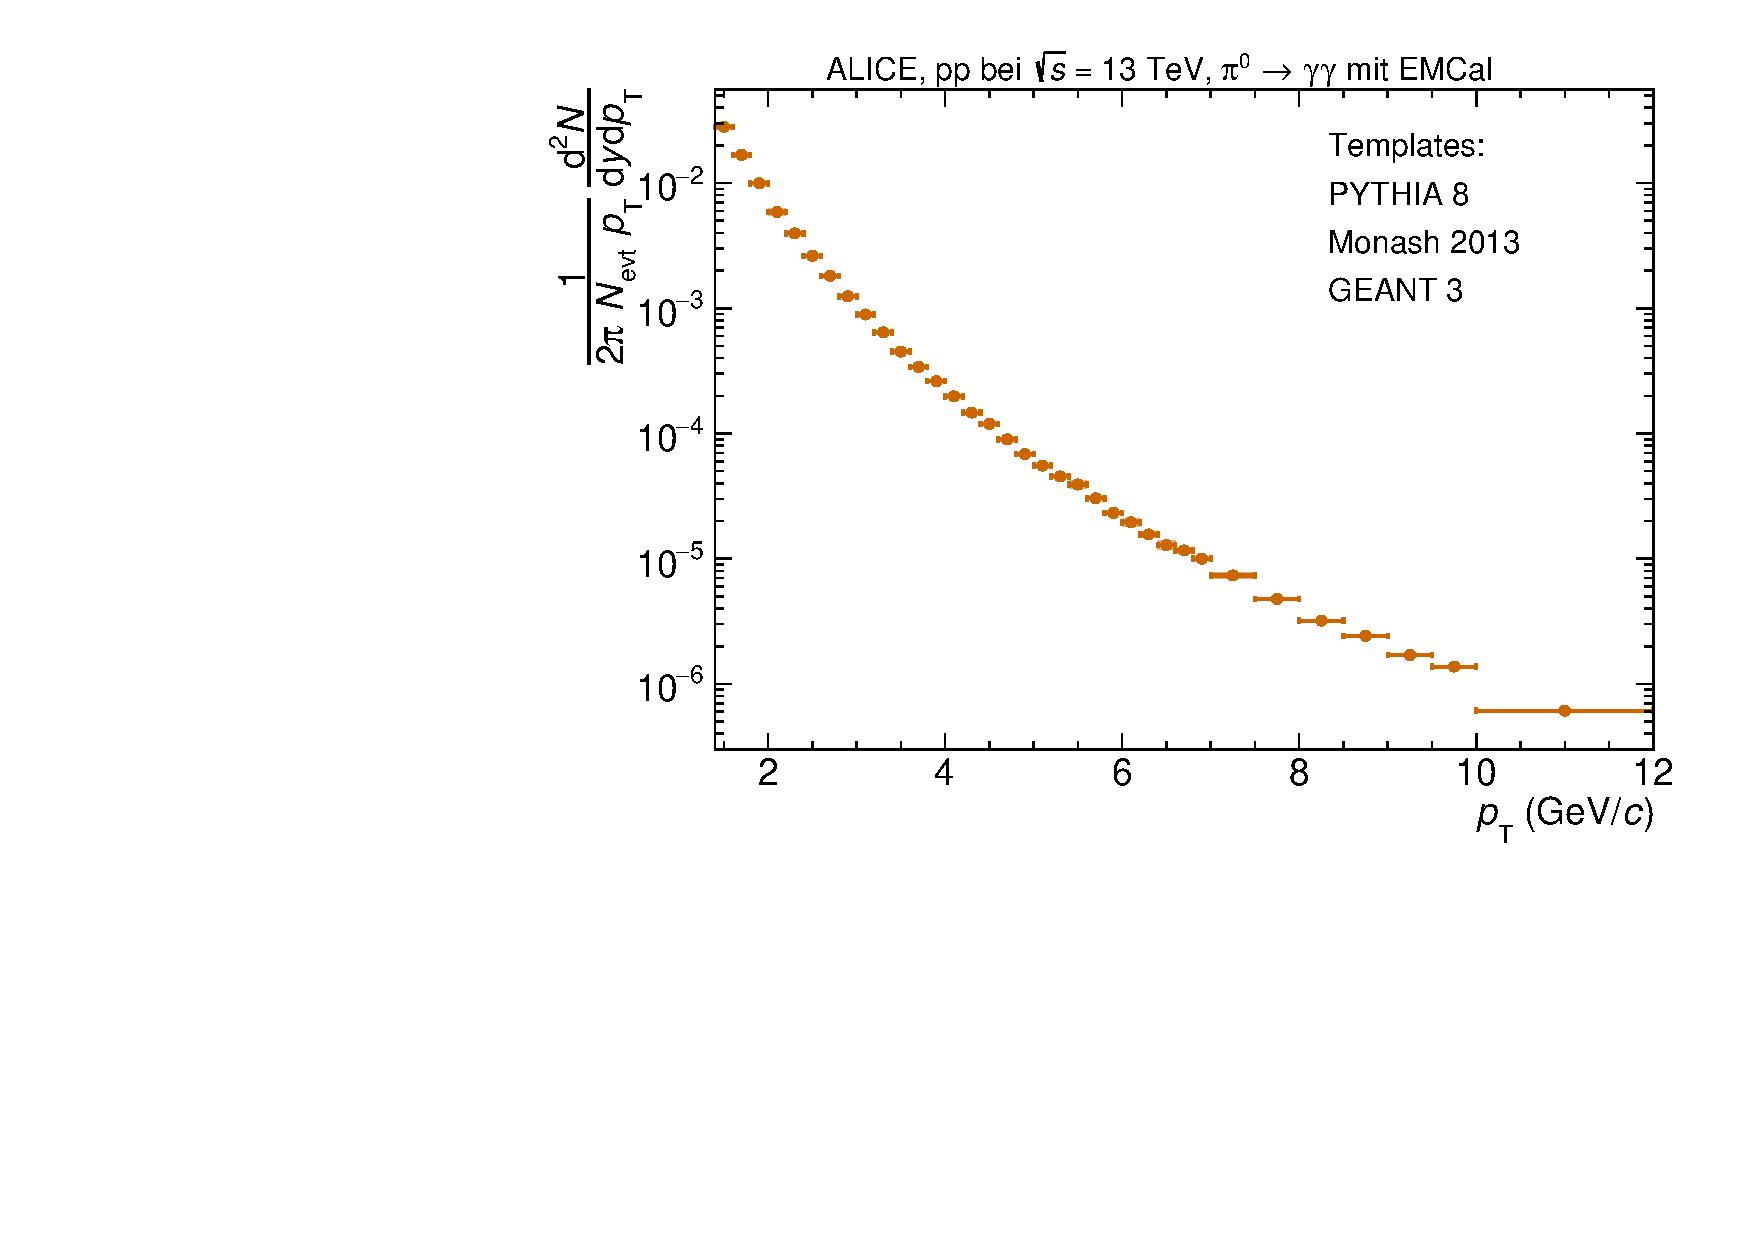
\includegraphics[width=.65\linewidth]{KorrigierterYield_Data_2016.pdf}
\caption{Korrigiertes $p_\text{T}$-Spektrum mit systematischer und statistischer Unsicherheit.}
\label{fig:KorrYield}
\end{figure}
\newline
Abbildung \ref{fig:KorrYield} zeigt das korrigierte $p_\text{T}$-Spektrum mit statistischer und systematischer Unsicherheit.
Die statistische Unsicherheit wird durch die vertikalen Linien, die systematische Unsicherheit durch die farbigen Boxen dargestellt.
\newline
Das korrigierte $p_\text{T}$-Spektrum wird im folgenden Abschnitt mit dem Ergebnis der Standardmethode verglichen.

\section{Vergleich mit Standardmethode} \label{s4s3}
\begin{figure}[t!]
\centering
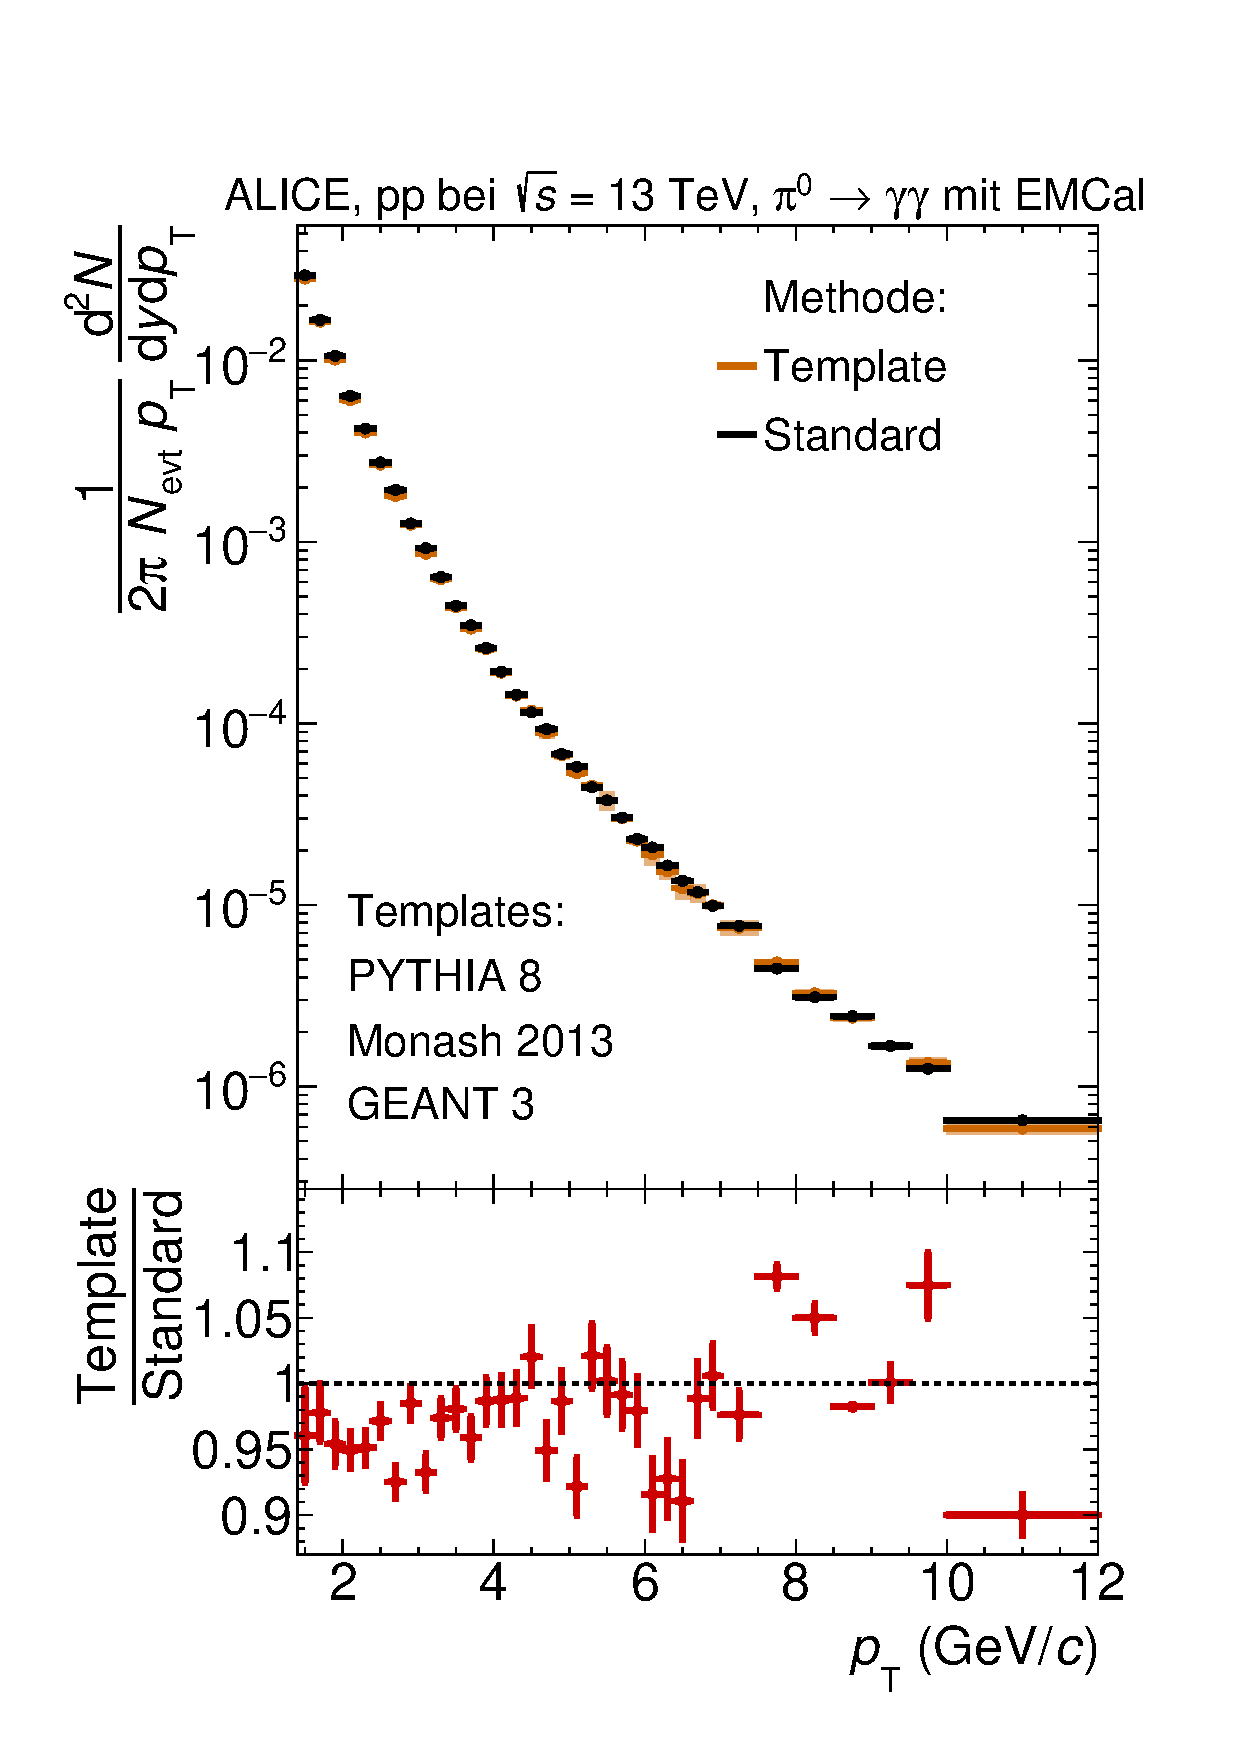
\includegraphics[width=.65\linewidth]{KorrigierteYields_Data_2016.pdf}
\caption{Korrigierte $p_\text{T}$-Spektren aus der Template Methode sowie aus der Standardmethode.
Außerdem das Verhältnis der beiden Spektren.}
\label{fig:KorrYieldComp}
\end{figure}
Abbildung \ref{fig:KorrYieldComp} zeigt das korrigierte $p_\text{T}$-Spektrum aus der Template Methode zusammen mit dem korrigierte $p_\text{T}$-Spektrum aus der Standardmethode.
Außerdem zeigt die Abbildung das Verhältnis von ersterem zu letzterem.
Das Verhältnis zeigt eine Diskrepanz zwischen den beiden Spektren von durchschnittlich etwa $3\%$ auf.
Im Bereich von $3,8 \leq p_\text{T}/\text{ (GeV}/c) < 5,8$ liegt das Verhältnis innerhalb der statistischen Unsicherheiten auf $1$.
Der größte Unterschied zwischen den Spektren beträgt etwa $10\%$, wo die statistischen Unsicherheiten der beiden Spektren den Unterschied nicht abdecken.
Mit Hilfe der systematischen Unsicherheit neben den statistischen Unsicherheit sollte sich eine gute Übereinstimmung der beiden Spektren ergeben.
\begin{figure}[t!]
\centering
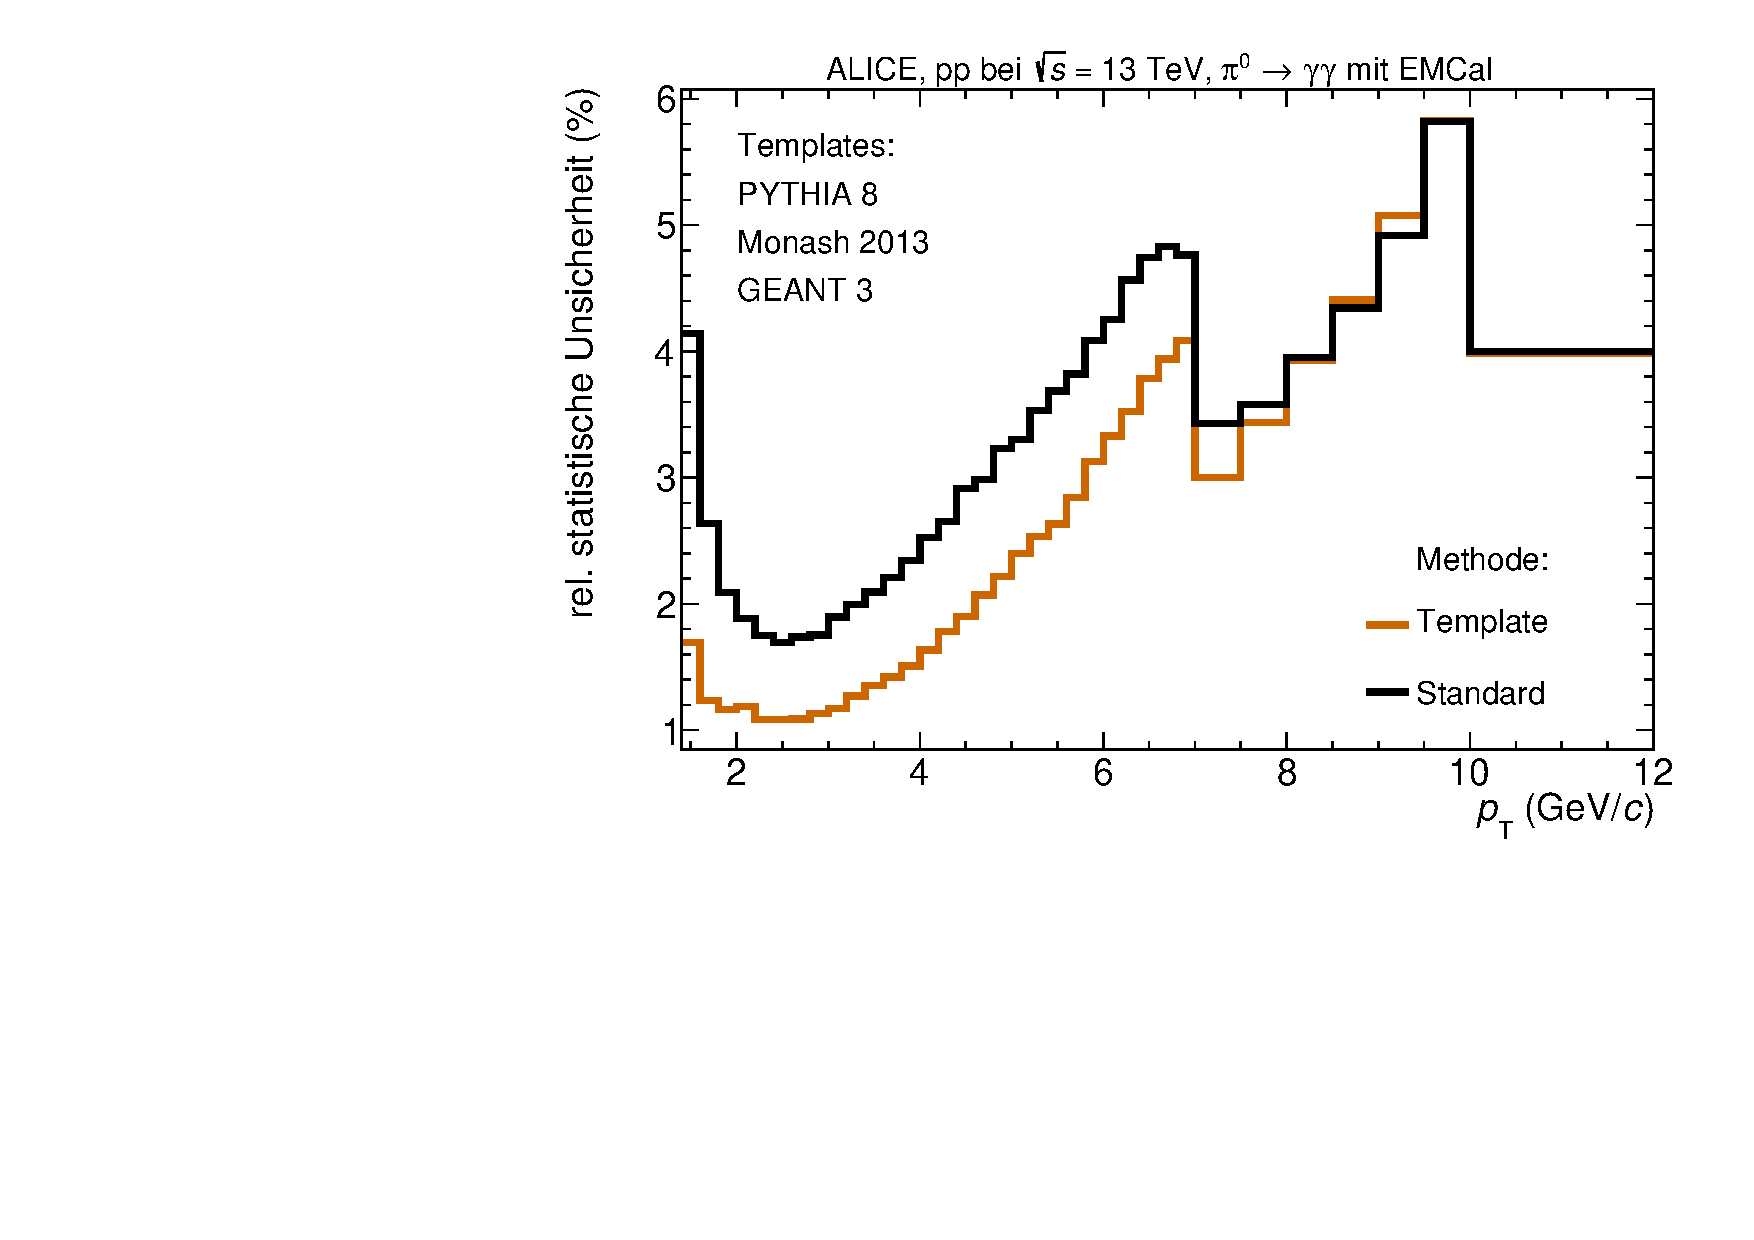
\includegraphics[width=.65\linewidth]{StatistischeUnsicherheitVergleich_Data_2016.pdf}
\caption{Statistische Unsicherheit der korrigierten $p_\text{T}$-Spektren aus der Analysemethode mit Templates, sowie aus der Standardmethode in Abhängigkeit von $p_\text{T}$.}
\label{fig:StatUncer}
\end{figure}
\newline
Abbildung \ref{fig:StatUncer} zeigt die statistischen Unsicherheiten der Spektren der beiden Methoden.
Der Verlauf der statistischen Unsicherheiten weist große Ähnlichkeit auf.
Über fast den gesamten $p_\text{T}$-Bereich hat die Template Methode eine geringe statistische Unsicherheit, als die Standardmethode.
Die geringere statistische Unsicherheit bei der Template Methode kommt von dem großen Zählbereich, der mit  dieser Methode möglich ist, sowie aus dem Konversionsanteil des Signals.
Zuvor wurde bereits gezeigt, dass die Standardmethode diesen Anteil des Signals unterschätzt.
\newline
Aufgrund der geringeren statistischen Unsicherheit der Template Methode, sowie der guten Über\-ein\-stim\-mung mit der Standardmethode stellt die Tempalte Methode eine mögliche Alternative zur Standardmethode dar.
Dabei kann sie entweder als neuer Standard für die Analyse von $\pi^{0}$ in pp-Kollisionen benutzt werden, oder als eine Variation für die Bestimmung der systematischen Unsicherheiten.
%\newline
%Außerdem zeigt der Vergleich der beiden Methoden, dass die Produktion von $\pi^{0}$ in pp-Kollisionen theoretisch gut verstanden wurde, da die Templates aus einer Monte Carlo Simulation entstanden.

\chapter{Zusammenfassung und Ausblick} \label{s5}
In der vorliegenden Arbeit werden Daten von pp-Kollisionen bei $\sqrt{s}=13\text{ TeV}$ analysiert.
Die Daten sind im Jahr 2016 mit dem ALICE-Experiment aufgezeichnet worden.
Bei dieser Arbeit handelt es sich um eine Analyse neutraler $\pi^{0}$ aus Messungen des EMCals mit Templates. %aus einer Monte Carlo Simulation.
\newline
%Zunächst werden die Zellen des EMCals, die Energie gespeichert haben, zu \textit{Clustern} zusammengefasst.
Um \textit{Cluster}, denen Photonen zugrunde liegen, von anderen \textit{Clustern} zu unterscheiden, werden verschiedene Anforderungen an die \textit{Cluster} gestellt.
Die so selektierten \textit{Clustern} werden anschließend in der \textit{same Event} Methode paarweise miteinander kombiniert und $p_\text{T}$ sowie $m_\text{inv}$ der \textit{Clusterpaare} berechnet.
\newline
Die daraus entstandene Verteilung der invarianten Masse und des Transversalimpulses besteht aus rekonstruierten $\pi^{0}$ und Untergrund.
Der Untergrund teilt sich in zwei Komponenten auf, den kor\-re\-lier\-ten und den unkorrelierten Untergrund.
Im Rahmen dieser Analyse werden die Verteilungen in 35 $p_\text{T}$-Intervalle aufgeteilt und einzeln betrachtet.
\newline
Um den unkorrelierten Untergrund abzuschätzen, werden \textit{Cluster} aus unterschiedlichen Events in der \textit{mixed Event} Methode miteinander kombiniert und skaliert.
Die skalierte Verteilung der invarianten Masse aus der \textit{mixed Event} Methode wird von der Verteilung der invarianten Masse aus der \textit{same Event} abgezogen.
\newline
Die verbleibende Verteilung wird in dieser Arbeit durch Templates beschrieben.
Die Templates werden aus der Information der Monte Carlo Simulation gewonnen.
Für jedes $p_\text{T}$-Intervall wird dabei ein eigenes Template des Signals verwendet, während es ein Template des korrelierten Untergrunds gibt, das für alle $p_\text{T}$-Intervalle verwendet wird.
Das Template des korrelierten Untergrunds wird mit Hilfe einer speziell für diesen Zweck angepassten Monte Carlo Simulation an die einzelnen $p_\text{T}$-Intervalle angepasst.
Diese Anpassung wird benötigt, da die Anforderung an den Öffnungswinkel zwischen zwei Photonen in einer $p_\text{T}$ abhängige untere Grenze für $m_\text{inv}$ resultiert.
\newline
Um die Templates an die Daten anzupassen werden diese mittels einer $\chi^{2}$-Minimierung parametrisiert.
Das skalierte Template des korrelierten Untergrunds, wird von der Verteilung der invarianten Masse der Daten ohne unkorrelierten Untergrund subtrahiert.
Die übrige Verteilung der Daten, das Signal, wird anschließend über einen festen $m_\text{inv}$-Bereich integriert und damit die Anzahl rekonstruierter $\pi^{0}$ in Abhängigkeit von $p_\text{T}$ bestimmt.
\newline
Das so extrahierte $p_\text{T}$-Spektrum wird anschließend auf die Detektorakzeptanz und die Rekonstruktionseffizienz korrigiert.
Durch Variationen in der Signalextraktion wird anschließend die systematische Unsicherheit im korrigierten $p_\text{T}$-Spektrum bestimmt.
\newline
Abschließend wird das korrigierte $p_\text{T}$-Spektrum aus der Analyse mit Hilfe von Monte Carlo Templates mit dem korrigierten $p_\text{T}$-Spektrum der Analyse mittels von Funk\-ti\-ons\-pa\-ra\-me\-tri\-sie\-rung verglichen.
Die Abweichung der beiden Spektren liegt im Bereich von $3\%$ und das Verhältnis der beiden Spektren ist innerhalb der statistischen Unsicherheit mit eins vereinbar.
Zuletzt wird die statistische Unsicherheit der beiden Analysemethoden verglichen.
Dabei zeigt sich, dass die Analyse mit Hilfe von Monte Carlo Templates fast in allen $p_\text{T}$-Intervallen geringere statistische Unsicherheiten hat als die andere Analysemethode.
\newline
Für einen vollständigen Vergleich der beiden Methoden wird noch die systematische Unsicherheit der Analyse mit Funktionsparametrisierung benötigt.
Außerdem kann die Analyse mit Templates noch erweitert werden, indem der unkorrelierte Untergrund ebenfalls durch die Verwendung eines Templates zusammen mit dem Template des Signals und dem Templates des korrelierten Untergrunds parametrisiert wird.
\clearpage

\appendix
\chapter{} \label{Appendix:A}
\begin{table}[]
	\centering

	\begin{tabular}{ | c || r | r ||  l  || c || r | r | }
		\hline
		Binnumber & Int Value & Error Value & \ & Binnumber & Int Value & Error Value \\ \hline
		1,4 - 1,6 & 8183,77 \  & 248,36 \hspace{3mm}  & \ &  5,0 - 5,2 & 375,78 \, & 76,18 \hspace{3mm} \\ \hline
		1,6 - 1,8 & 12696,80 \ & 319,21 \hspace{3mm} & \ &  5,2 - 5,4 & 183,20 \, & 70,98 \hspace{3mm} \\ \hline
		1,8 - 2,0 & 14928,40 \ & 335,82 \hspace{3mm} & \ &  5,4 - 5,6 & 273,14 \, & 64,85 \hspace{3mm} \\ \hline
		2,0 - 2,2 & 13686,40 \ & 323,90 \hspace{3mm} & \ &  5,6 - 5,8 & 105,55 \, & 61,23 \hspace{3mm} \\ \hline
		2,2 - 2,4 & 10766,10 \ & 300,70 \hspace{3mm} & \ &  5,8 - 6,0 & 106,59 \, & 56,42 \hspace{3mm} \\ \hline
		2,4 - 2,6 & 9047,53 \  & 273,67 \hspace{3mm} & \ &  6,0 - 6,2 & 34,35 \& 52,23 \hspace{3mm} \\ \hline
		2,6 - 2,8 & 6901,65 \  & 246,32 \hspace{3mm} & \ &  6,2 - 6,4 & 3,41 \ & 49,94 \hspace{3mm} \\ \hline
		2,8 - 3,0 & 5429,20 \  & 221,03 \hspace{3mm} & \ &  6,4 - 6,6 & 8,73 \   & 46,40 \hspace{3mm} \\ \hline
		3,0 - 3,2 & 4220,52 \  & 198,67 \hspace{3mm} & \ &  6,6 - 6,8 & -23,16 \ & 43,73 \hspace{3mm} \\ \hline
		3,2 - 3,4 & 3253,74 \ & 178,66 \hspace{3mm} & \ &  6,8 - 7,0 & -13,32 \ & 40,78 \hspace{3mm} \\ \hline
		3,4 - 3,6 & 2660,09 \ & 160,66 \hspace{3mm} & \ &  7,0 - 7,5 & -47,53 \ & 56,97 \hspace{3mm} \\ \hline
		3,6 - 3,8 & 1994,75 \ & 144,91 \hspace{3mm} & \ &  7,5 - 8,0 & -35,33 \ & 49,50 \hspace{3mm} \\ \hline
		3,8 - 4,0 & 1537,27 \ & 130,91 \hspace{3mm} & \ &  8,0 - 8,5 & -79,79 \ & 42,67 \hspace{3mm} \\ \hline
		4,0 - 4,2 & 1411,16 \ & 118,39 \hspace{3mm} & \ &  8,5 - 9,0 & -85,09 \, & 39,43 \hspace{3mm} \\ \hline
		4,2 - 4,4 & 852,25 \  & 108,17 \hspace{3mm} & \ &  9,0 - 9,5 & -39,02 \, & 35,48 \hspace{3mm} \\ \hline
		4,4 - 4,6 & 817,07 \  & 99,02 \hspace{3mm} &  \ &  \, 9,5 - 10,0 & -32,65 \, & 31,98 \hspace{3mm} \\ \hline
		4,6 - 4,8 & 590,26 \  & 89,73 \hspace{3mm} &  \ &  10,0 - 12,0 & -288,32 \,& 50,04 \hspace{3mm} \\ \hline
		4,8 - 5,0 & 460,15 \  & 82,49 \hspace{3mm} &  \ & \   & \  & \  \\ \hline
	
	\end{tabular}
	
	\caption{Integral und Unsicherheit der Templates des korrelierten Untergrunds}
	\label{tab:IntAndError}
	
\end{table}
\newpage
\bibliography{bib_bath_mahe} 
\bibliographystyle{alpha}
\clearpage
\chapter{Danksagung} \label{Appendix:B}
Zuallererst möchte ich mich bei Prof. Dr. Henner Büsching bedanken, der mich in seiner Gruppe aufgenommen hat und mir dadurch ermöglicht hat diese Arbeit schreiben zu können.
Er stand außerdem jederzeit für Fragen zur Verfügung, sowohl bezüglich physikalischer Natur, als auch bei Fragen bezüglich des Schreibens.
\newline
Mein weiterer Dank gilt Fabian Pliquett, der zusammen mit Prof. Dr. Büsching viel Zeit aufgewandt hat, um mir unter anderem die Bedeutung von Präzision und Konsistenz näher zu bringen, dir mir nicht nur für diese Arbeit, sondern auch für mein weiteres Arbeitsleben nützlich sein wird.
\newline
Neben Fabian möchte ich mich auch bei meiner Bürokollegin Kristina Schmitt und meinen Büro\-kol\-le\-gen Sebastian Scheid, Patrick Reichelt und Janik Ditzel, die für ein angenehmes Arbeitsklima gesorgt haben, in zweifacher Hinsichten.
\newline
Weiterhin möchte ich mich bei meinem Betreuer Joshua König bedanken, der von Anfang an ein offenes Ohr für alle meine Fragen hatte und mir stets Anregungen gegeben hat, wenn ich mal nicht weiter wusste.
\newline
Außerdem hat Joshua zusammen mit Adrian Mechler mir den Einstieg in die Arbeitsgruppe sowie in das Arbeiten mit C++ und root erleichtert, weshalb auch ihm Dank gebührt.
\newline
Mein Dank gilt auch Andrea Hornung, die mir, wie Joshua, sowohl bei Fragen bezüglicher der Analyse, als auch bei Fragen rund ums Schreiben geholfen hat.
\newline
Weiterhin möchte ich mich bei der gesamten Hochenergiephysik-Gruppe am IKF bedanken, die mich freundlich aufgenommen und mir hilfreiches Feedback für meine Arbeit gegeben hat, sowie für einige schöne Momente gesorgt hat.
\newline 
Ein großer Dank gilt auch meiner Familie, die mir unter der Präsumtion, dass ich mein Studium erfolgreich abschließen kann, sowohl moralisch als auch finanziell zur Seite stehen und durch deren Unterstützung mein Studium überhaupt erst möglich wurde.
\newline
Zuletzt möchte ich mich noch bei meinen Freunden Florian Zindel, Katharina Zoch, Jan Röder und Julia Lienert bedanken, die mich während des Studiums und vor allem während des Schreibens dieser Arbeit unterstützt haben.

\end{document}
